%% ****** Start of file apstemplate.tex ****** %
%%
%%
%%   This file is part of the APS files in the REVTeX 4.2 distribution.
%%   Version 4.2a of REVTeX, January, 2015
%%
%%
%%   Copyright (c) 2015 The American Physical Society.
%%
%%   See the REVTeX 4 README file for restrictions and more information.
%%
%
% This is a template for producing manuscripts for use with REVTEX 4.2
% Copy this file to another name and then work on that file.
% That way, you always have this original template file to use.
%
% Group addresses by affiliation; use superscriptaddress for long
% author lists, or if there are many overlapping affiliations.
% For Phys. Rev. appearance, change preprint to twocolumn.
% Choose pra, prb, prc, prd, pre, prl, prstab, prstper, or rmp for journal
%  Add 'draft' option to mark overfull boxes with black boxes
%  Add 'showkeys' option to make keywords appear
%\documentclass[aps,prb,preprint,groupedaddress]{revtex4-2}
%\documentclass[aps,prl,preprint,superscriptaddress]{revtex4-2}
\documentclass[aps,prb,reprint,superscriptaddress]{revtex4-2}
% Enable some packages (same as my 8.06x paper)
\usepackage{blindtext}
\usepackage{mathtools}
\usepackage{graphicx}
\usepackage{amsmath}
\usepackage{amsfonts}
\usepackage{amssymb}
\usepackage{amstext}
\usepackage[english]{babel}
\usepackage{helvet}
\usepackage{microtype}
% \usepackage[pdftex]{hyperref}
\usepackage[hidelinks]{hyperref}
\usepackage{bbold}
\usepackage{mathrsfs}

\DeclareMathOperator{\Tr}{Tr}
% Some new commands
\newcommand{\rgeq}{\stackrel{\text{RG}}{=}}
\newcommand{\defeq}{\stackrel{\text{def}}{=}}
\newcommand{\svdeq}{\stackrel{\text{svd}}{=}}
\newcommand{\rgapprox}{\stackrel{\text{RG}}{\approx}}
\newcommand{\ket}[1]{|#1\rangle}
\newcommand{\bra}[1]{\langle#1|}
\newcommand{\textapprox}[1]{\stackrel{\text{#1}}{\approx}}


% You should use BibTeX and apsrev.bst for references
% Choosing a journal automatically selects the correct APS
% BibTeX style file (bst file), so only uncomment the line
% below if necessary.
%\bibliographystyle{apsrev4-2}

\begin{document}

% Use the \preprint command to place your local institutional report
% number in the upper righthand corner of the title page in preprint mode.
% Multiple \preprint commands are allowed.
% Use the 'preprintnumbers' class option to override journal defaults
% to display numbers if necessary
%\preprint{}

%Title of paper
\title{Scaling dimensions from analyzing tensor renormalization group
flow}

% repeat the \author .. \affiliation  etc. as needed
% \email, \thanks, \homepage, \altaffiliation all apply to the current
% author. Explanatory text should go in the []'s, actual e-mail
% address or url should go in the {}'s for \email and \homepage.
% Please use the appropriate macro foreach each type of information

% \affiliation command applies to all authors since the last
% \affiliation command. The \affiliation command should follow the
% other information
% \affiliation can be followed by \email, \homepage, \thanks as well.
\author{Xinliang Lyu}
\email[]{lyu@issp.u-tokyo.ac.jp}
%\homepage[]{Your web page}
%\thanks{}
%\altaffiliation{}
\affiliation{Institute for Solid State Physics, The University of Tokyo,
Kashiwa, Chiba 277-8581, Japan}
\author{RuQing Xu}
%\email[]{r-xu@g.ecc.u-tokyo.ac.jp}
\affiliation{Department of Physics, The University of Tokyo, Tokyo
113-0033, Japan}
\author{Naoki Kawashima}
\email[]{kawashima@issp.u-tokyo.ac.jp}
\affiliation{Institute for Solid State Physics, The University of Tokyo,
Kashiwa, Chiba 277-8581, Japan}


%Collaboration name if desired (requires use of superscriptaddress
%option in \documentclass). \noaffiliation is required (may also be
%used with the \author command).
%\collaboration can be followed by \email, \homepage, \thanks as well.
%\collaboration{}
%\noaffiliation

\date{\today}

\begin{abstract}
    Here is the abstract.
% insert abstract here
\end{abstract}

% insert suggested keywords - APS authors don't need to do this
%\keywords{}

%\maketitle must follow title, authors, abstract, and keywords
\maketitle

% body of paper here - Use proper section commands
% References should be done using the \cite, \ref, and \label commands
\section{Introduction\label{intro}}
% Put \label in argument of \section for cross-referencing
%\section{\label{}}
% Insert subsection and subsubsection
%\subsection{}
%\subsubsection{}
Renormalization group (RG) is a powerful technique to study physical
systems where fluctuations in all scales of length are
important~\cite{wilsonNobel}. In statistical mechnaics, the most famous
example is critical phenomena. Take water as an example, imagine the
temperature and pressure are increased along the liquid-vapor
coexistence line, when we reach a temperature of $374^\circ$C and
pressure of $218$ atm, the distinction between liquid and vapor starts
vanishing and the density of water flucuates at all length scales. The
deisnty fluctuations with the order of hundreds of nanometers will
scatter visible light strongly. The water will look milky due to such
fluctuations. RG can be applied to critical phenomena like this and can
make nice predictions that agree with experiments. 
%

The main idea behind RG is to study how a physical system changes as we
go from one length scale to another. In conventional approach, the
goal is usually to find a mapping from the Hamiltonian of the
old length scale to that of the new length scale such that the partition
function is unchanged~\cite{nonlinearRG}. The mapping is known as an RG
equation. In principle, the exact RG equation is a transformation from
an infinite dimensional space to another infinite dimensional
space~\cite{wilsonNobel,wilson1970a}. In order to perform a practical
calculation, approximation is necessary. In early stage of the
development of RG, the schemes include $\epsilon$
expansion~\cite{wilson1972}, $1/n$ expansion~\cite{largeNexp} and spin
block
method~\cite{kadanoff1966,kadanoff1975,migdal,kadanoff1976,niemeijer1973}.
They all have their own strengths and limitations. $\epsilon$ expansion
works better if $\epsilon$ takes a small value such as $1$. $1/n$
expansion is similar, but for relative large values of $n$. Potential
moving trick for spin block method is simple but there is no systematic
way to improve the approximation~\cite{kardar2007}.
%

Recently, ideas from quantum information have stimuated a novel class of
RG method. Instead of finding a mapping from an old Hamiltonian to a new
Hamiltonian, this new type of method seeks a mapping from a tensor
encapsulating Boltzmann weight of local configurations at the old length
scale to a new tensor at the new length scale. The first realization of
this new paradigm is tensor renormalization group (TRG) proposed by
Levin and Nave~\cite{trg} in 2007. It is designed for classical
statistical lattice models in 2D.
TRG has excellent performance in calculations of free energy. The
approximation is controlled by one integer parameter called bound
dimension, often denoted as $\chi$. Larger the value of $\chi$, more
time the computation takes, better the approximation becomes and more
accurate estimation of free energy is achieved. Later, people realized
that even better approximation can be achieved by considering larger
environment~\cite{SRGa,SRGb,hotrg,morita2020global}. With the help of
these TRG-type techniques, we can easily calculate the free energy of,
for example, Ising model in 2d, with the error of the order $10^{-7}$
within a few minutes in a desktop computer. The accuracy improves
exponentially as $\chi$ increases, while the computation cost only grows
polynomially. Later, generalizations of TRG that are also applicable for
3D systems were found~\cite{hotrg,atrg,triadtrg}, the earliest of which
is higher-order tensor renormalization group (HOTRG)~\cite{hotrg}
proposed in 2012.
%

With all of their success in calculating free energy, however, TRG-type
techniques are lack of one nice feature of the conventional RG approach.
RG equation in old approach usually gives fixed points. It is now
understood that different fixed points correspond to different conformal
field theories (CFTs)~\cite{polchinski1988,nakayama2015}. By studying
the RG equation linearized around a critical fixed point, scaling
dimensions of the local operators in the corresponding CFT can be
extracted directly. The critical exponents are then calculated using
these scaling dimensions and can be compared with values in expreimental
measurements. However, in the new TRG-type calculations, the
abovementioned fixed point analysis is more subtle and
difficult~\cite{kadanoff2014}.  Instead, some of the critical exponents
can be calculated by obtaining free energy first and then taking
derivatives of the free energy with respect to various parameters like
temperature and external magnetic field~\cite{hotrg,
Berker2008,xiang2019adtrg}. 
%

Several attempts were made to perform fixed point analysis in the new
TRG-type calculations. In 2008, just one year after Levin and Nave
proposed TRG, Hinczewski and Berker~\cite{Berker2008} first analyzed the
tensor RG flow generated by the new method. What they discovered is
extremely interesting.  By fine-tuning the temperature of 2d Ising model
on a triangular lattice, they found that for bound dimension $\chi \leq
8$, the tensor would flow to the critical fixed point before flowing
alway to high and low temperature trivial fixed point. When they
increased the bound dimension to $\chi =  12$ and further, the tensor
would never flow to the critical fixed point tensor before flowing alway
to trivial fixed points. It means that TRG fails to exhibit critical
fixed points. Most physicists might be unware of such difficulty since
it seldom occurs in the conventional approach, but Wilson did notice
this and called it ``a serious problem with the renormalization-group
transformations'' in his 1982 Nobel prize lecture~\cite{wilsonNobel}.
Since this serious problem shows itself in the TRG-type calculations
when $\chi > 8$, the subsequent attempts only focused on very small
bound dimensions like $\chi = 2, 3$ or $4$ either using
TRG~\cite{kadanoff2014,aoki2009} or HOTRG~\cite{meurice2013}. Three of
them~\cite{Berker2008,aoki2009,meurice2013} are only able to calculate
the scaling dimension of the energy density operator in 2D Ising at
criticality, and the accuracy is similar to old potential moving
schemes. One of them~\cite{kadanoff2014} is able to calculate the
scaling dimension of the spin operator, however, with more than a factor
of 2 larger than the exact value. 
%

Fortunately, in recently ten years, people have developed many tricks to
solve the serious problem of TRG-type methods. In 2009, Gu and
Wen~\cite{GuWen2009} provided the first detailed analysis on this. They
followed Levin's sugguestion~\cite{trg,LevinTalk} and focused on a toy
model called corner double-line (CDL) tensors, which represent systems
with only short-range interactions. They showed that TRG fails to
simplify CDL tensors so the short-range interactions in the smaller
length scale will be carried to the larger length scale. A relative
crude algorithm was proposed to filter CDL tensors and solved the
problem of tensor RG flow partially, followed up by an improved one in
2017~\cite{looptnr}. From 2015 to 2017, several similar methods were
proposed~\cite{tnr,tnralgo,tnrplus}. All of these algorithms are
designed for 2D systems and they all exhibit critical fixed point
tensors. In the 2009 paper, Gu and Wen~\cite{GuWen2009} pointed out that
a transfer matrix defined on a cylinder can be constructed from fixed
point tensors and the scaling dimensions of the corresponding CFTs can
be extracted by diagonalizing the transfer matrix according to a
well-known result in CFT in 2D~\cite{cardy1986}.  This method has been
applied to calculate scaling dimensions of 2D systems from then on,
while the fixed point analysis in tensor network language has never
followed up.
%

In this paper, we want to provide the missing piece of analyzing the
critical fixed points in the new TRG-type calculations with bound
dimension $\chi > 8$. On a practical level, it is a method to extract
scaling dimensions of local operators in a CFT in any dimension, while
the transfer matrix method is restricted in 2D CFTs. On a theoretical
level, more importantly, it accomplishes a important step of RG methods
in tensor network language.  Fixed point analysis is from pure RG
perspective, without reference to any CFT results. If the predictions of
fixed point analysis agree with those from CFT arguments, it provides
more evidence indicating the correspondence between an RG fix point and
a CFT~\cite{poland2019}.
%

% TODO
[\textbf{Outline of our paper and our main achievements}]


\section{Renormalization group transformation in tensor network
language\label{introTRG}}
In this section, we show how to rewrite the partition function $Z$ of
a 2D classical statistical system using tensor network representations.
Notice that the procedure works equally well for $1 + 1$D quantum
system, whose Euclidean path integral can have a tensor network
representation~\cite{GuWen2009}. [\textbf{Add more later...}]
% TODO
%
\subsection{From a lattice with statistical variables to a tensor
network\label{spin2tensor}}
We use the simpliest example, the 2D classical Ising model with only the
nearest-neighbor ferromagnetic interaction, to demonstrate how to find a
tensor network representation of a partition function. The 2D classical
Ising model will be our benchmark model in Sec.~\ref{benchmark:2DIsing}.
There are at least two ways to construct the tensor network. The method
introduced by Hauru, Delcamp and Mizera~\cite{gilts} is more general and
can be trivially adapted to apply on 3D classical Ising
model~\cite{hotrg} and other models like $\phi^4$ theory in
2D~\cite{Delcamp2020}. However, we will use the other method~\cite{trg,
tnr}, which is more straightforward and whose physical meaning is more
transparent.
%

Consider classical spin variables living on a sqaure lattice shown in
Fig.~\ref{fig:spin2tensor}. The square lattice is sketched with blue
dashed lines and the blue dots are where spin variables sit. The
partition function is
%
\begin{align}\label{eq:2DIsingZ}
    Z = \sum_{\{\sigma(\mathbf{r})\}}e^{K\sum_{\langle i,j
        \rangle}\sigma_i \sigma_j},
\end{align}
where $\sigma_i$ is the shorthand for the spin variable
$\sigma(\mathbf{r}_i)$ located at lattice point $\mathbf{r}_i$ and can
take values $\pm 1$, and $K = J / k_B T$. In this paper, we measure
temperature in units of $J / k_B $ so it becomes a dimensionless number.
% Figure: mapping from spins on lattice to a tensor network
\begin{figure}[htb]
    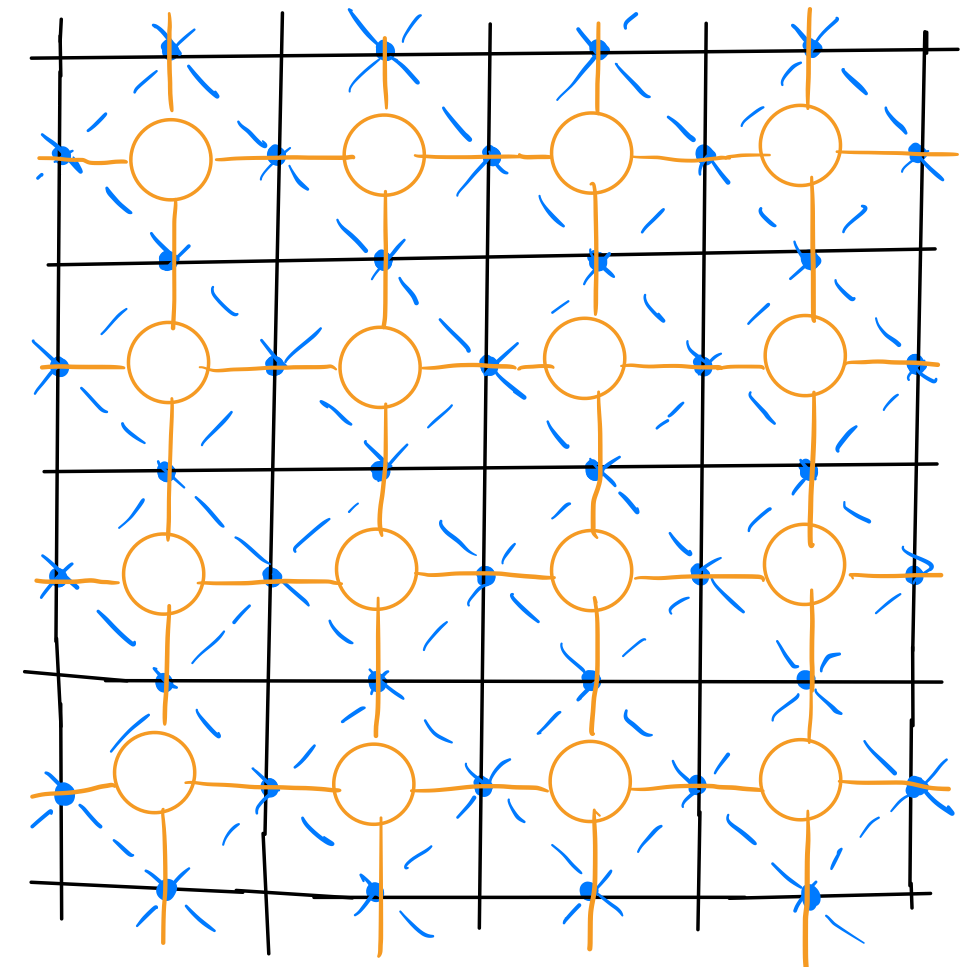
\includegraphics[width=6.5cm]{./figs/spin2tensor}
    \caption{\label{fig:spin2tensor}[\textbf{Add descriptions}]}
\end{figure}
% Figure end
%

Now, imagine dividing this
region into square blocks using the black solid lines in
Fig.~\ref{fig:spin2tensor}, such that each side of a black square
holds a spin variable. Finally, put a four-leg tensor (green circles
with four green legs) at the center of each black square, with its four
legs connected with the four spin variables on the sides of the black
square. The graph we get in green is the tensor network, where four-leg
tensors connected with each other to form a new square lattice. To
determine the values of a four-leg tensor, we simply divide the summation
on the exponential in Eq.~\eqref{eq:2DIsingZ} into groups where pairs of
spin variables are together if they belong to the same black square and
define such a Boltzmann weight as
%
\begin{align}\label{def:tensorA}
    A_{\sigma_i \sigma_j \sigma_k \sigma_l} &\defeq
    e^{K(\sigma_i\sigma_j + \sigma_j\sigma_k + \sigma_k\sigma_l +
    \sigma_l\sigma_i)}
    \nonumber\\ 
    &= 
    \begin{minipage}{2.0truecm}
      \centering
      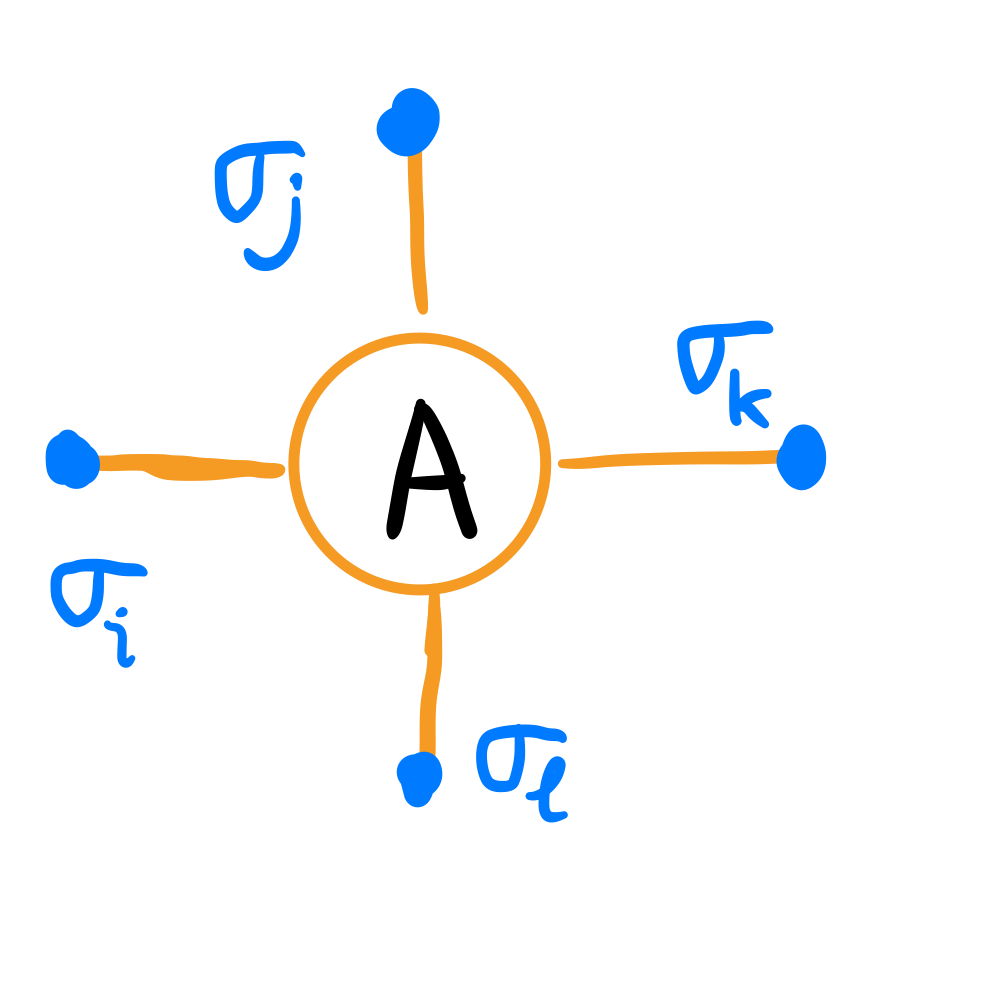
\includegraphics[width=2.0truecm,clip]{./figs/defAtensor}
    \end{minipage}.
\end{align}
%
Each index of this tensor can take two values $\pm 1$ and we say the
bound dimension of a leg of this tensor is $\chi = 2$. With this
definition of a four-leg tensor $A$, it is now possible to rewrite the
partition function of 2D Ising model in Eq.~\eqref{eq:2DIsingZ} as the
tensor product of all $A$ tensors inside the black squares, with all
their indices summed over
%
\begin{align}
    Z = \sum_{\{ \sigma(\mathbf{r}) \}} \bigotimes_{\square}A_{\sigma_i
    \sigma_j \sigma_k \sigma_l}.
\end{align}
%
As a concrete example, for a finite system defined in
Fig.~\ref{fig:spin2tensor} with periodic bound condition, the total
$4 \times 8 = 32$ spin variables are mapped into $4 \times 4 = 16$
tensor $A$'s. If we adopt the summation convention that the index is
summed over whenever the corresponding leg is shared by two tensors, the
partition function~\eqref{eq:2DIsingZ} now has a nice picturial
description
%
\begin{align}\label{eq:tensorZ4by4}
    Z_{4 \times 4} = 
    \begin{minipage}{2.4truecm}
      \centering
      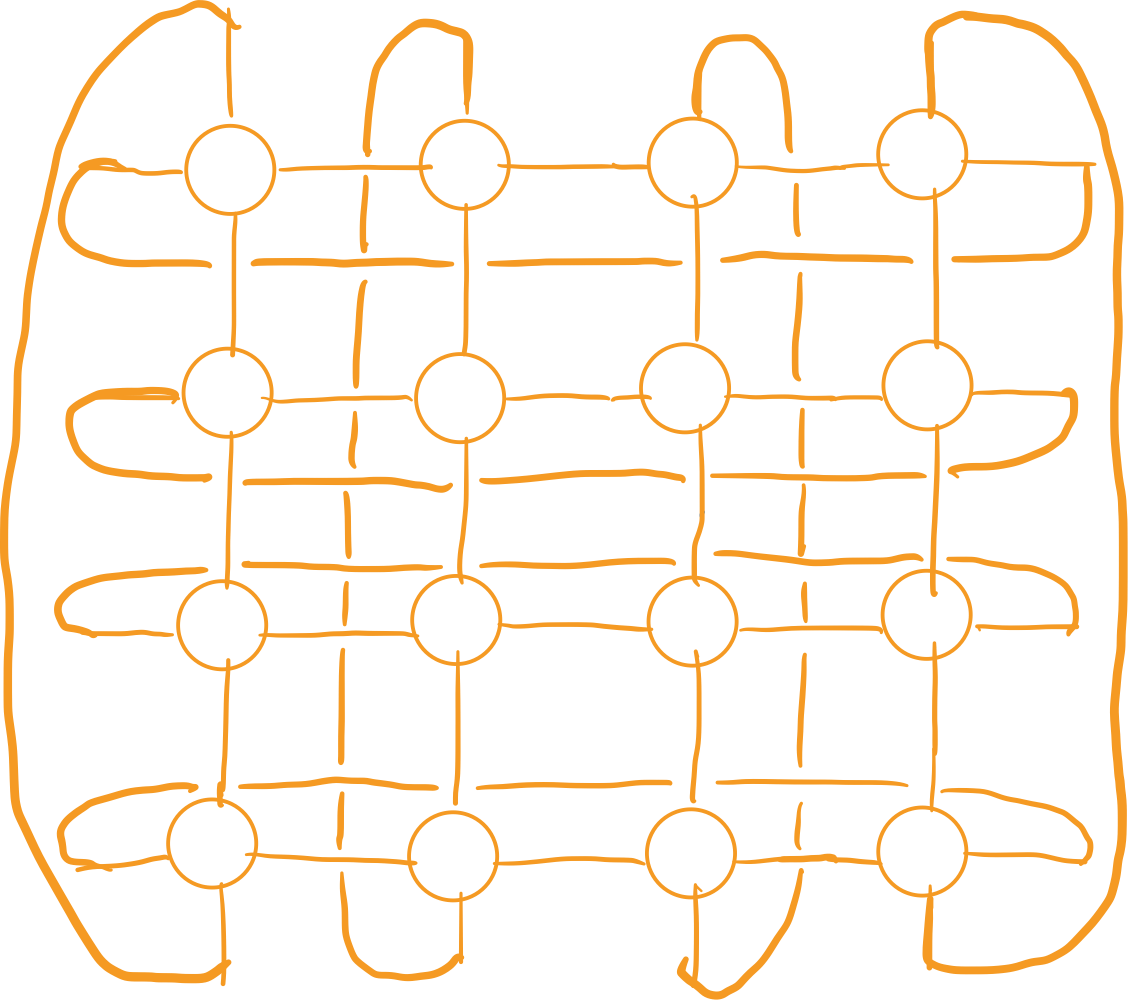
\includegraphics[width=2.3truecm,clip]{./figs/Z-TN}
    \end{minipage}.
\end{align}
%
Eq.~\eqref{eq:tensorZ4by4} above provides a tensor network representation of
the partition function~\eqref{eq:2DIsingZ}. It is the starting point of
all the TRG-type schemes. Notice that the number of tensors in the
tensor network is half of the number of spin variables. In addition, if
the lattice constant of the original spin system is $a/\sqrt{2}$ (that
is, the length of a side of a blue dashed square in
Fig.~\ref{fig:spin2tensor}), the distance of the nearest two tensors in
the resultant tensor network is $a/\sqrt{2} \times \sqrt{2} = a$.
It is worth to mention that all classical
models with local interactions have tensor network
representations for their partition functions~\cite{trg}. 

\subsection{Coarse graining a tensor network: a general
description\label{cgTN}}
The RG transformations in the tensor network representation are similar
to the conventional spin block methods. A transformation is usually
defined by grouping several old variables together to form a new
variable. The system described by the new variables will have a
different length scale (in particular, a difference lattice constant)
but the partition function should be the same as the system described by
the old variables. Interestingly, the RG transformations in the tensor
representation are easier to grasp and more transparent than in the
conventional approach. Let's focus on the concrete example whose
partition function is defined in Eq.~\eqref{eq:tensorZ4by4}. 
%

The system is originally described by sixteen $A$ tensors in
Eq.~\eqref{def:tensorA}. The simpliest way to carry on the coarse
graining is to blcok a square of four tensors by contracting legs
between them and group every two legs in the same side. Call the new
tensor $A_c$,
%
\begin{align}\label{eq:exactBlock}
    \begin{minipage}{2.0truecm}
      \centering
      
\includegraphics[width=1.7truecm,clip]{./figs/Ac-thickleg}
    \end{minipage}
    \defeq
    \begin{minipage}{2.0truecm}
      \centering
      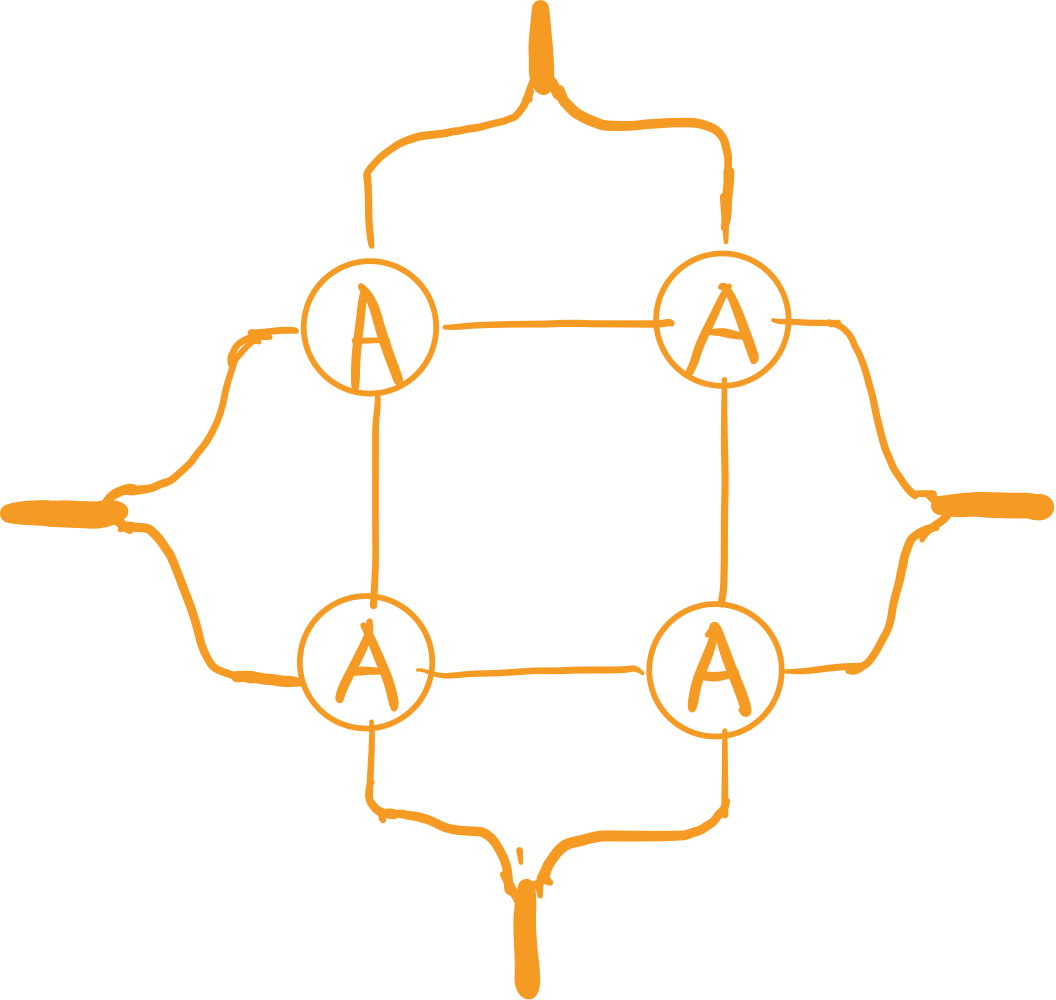
\includegraphics[width=2.0truecm,clip]{./figs/block4As}
    \end{minipage}.
\end{align}
%
Then, the partition function can be fully described by the new tensor
$A_c$ after the above coarse graining process
%
\begin{align}\label{eq:ZunderRG}
    Z_{4 \times 4} = 
    \begin{minipage}{2.4truecm}
      \centering
      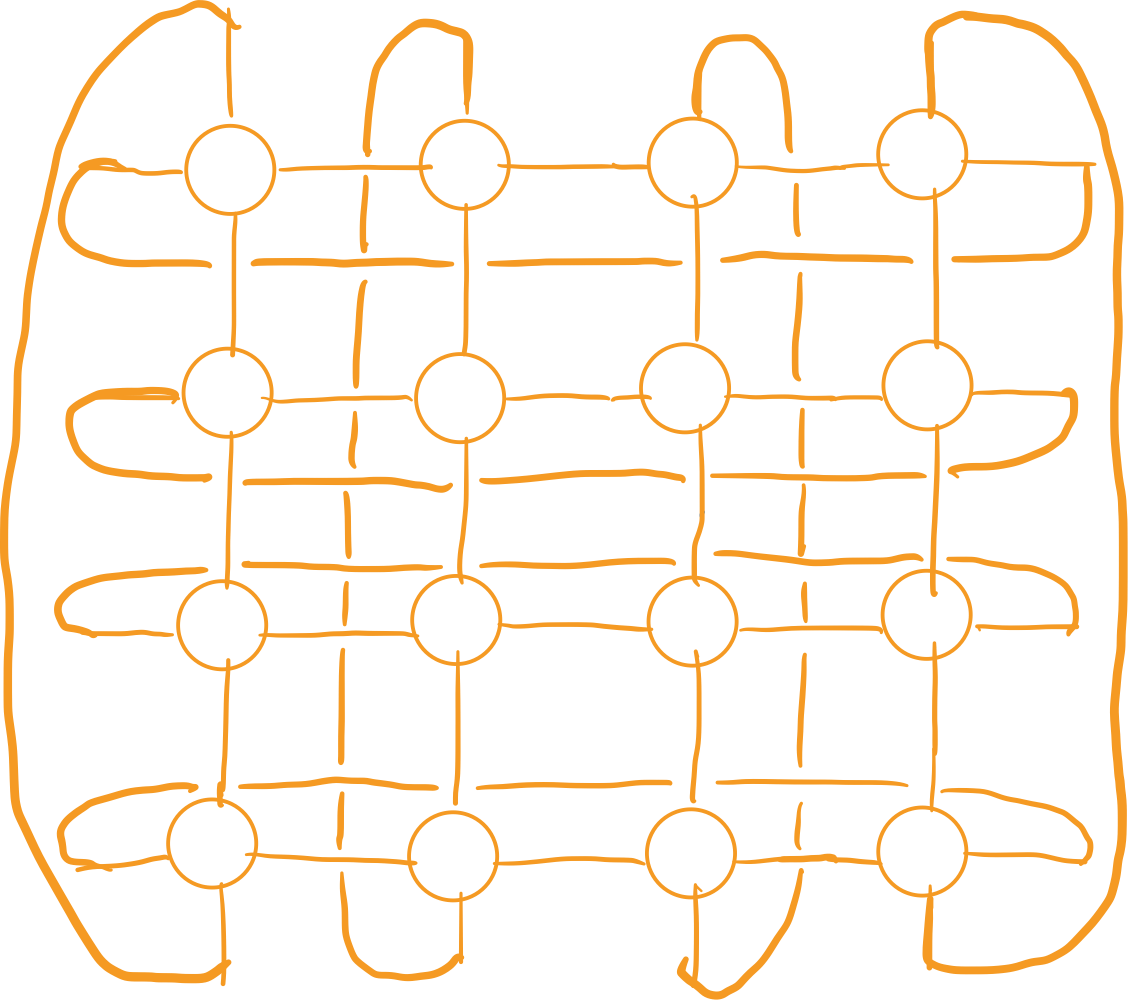
\includegraphics[width=2.3truecm,clip]{./figs/Z-TN}
    \end{minipage}
    \rgeq
    \begin{minipage}{2.6truecm}
      \centering
      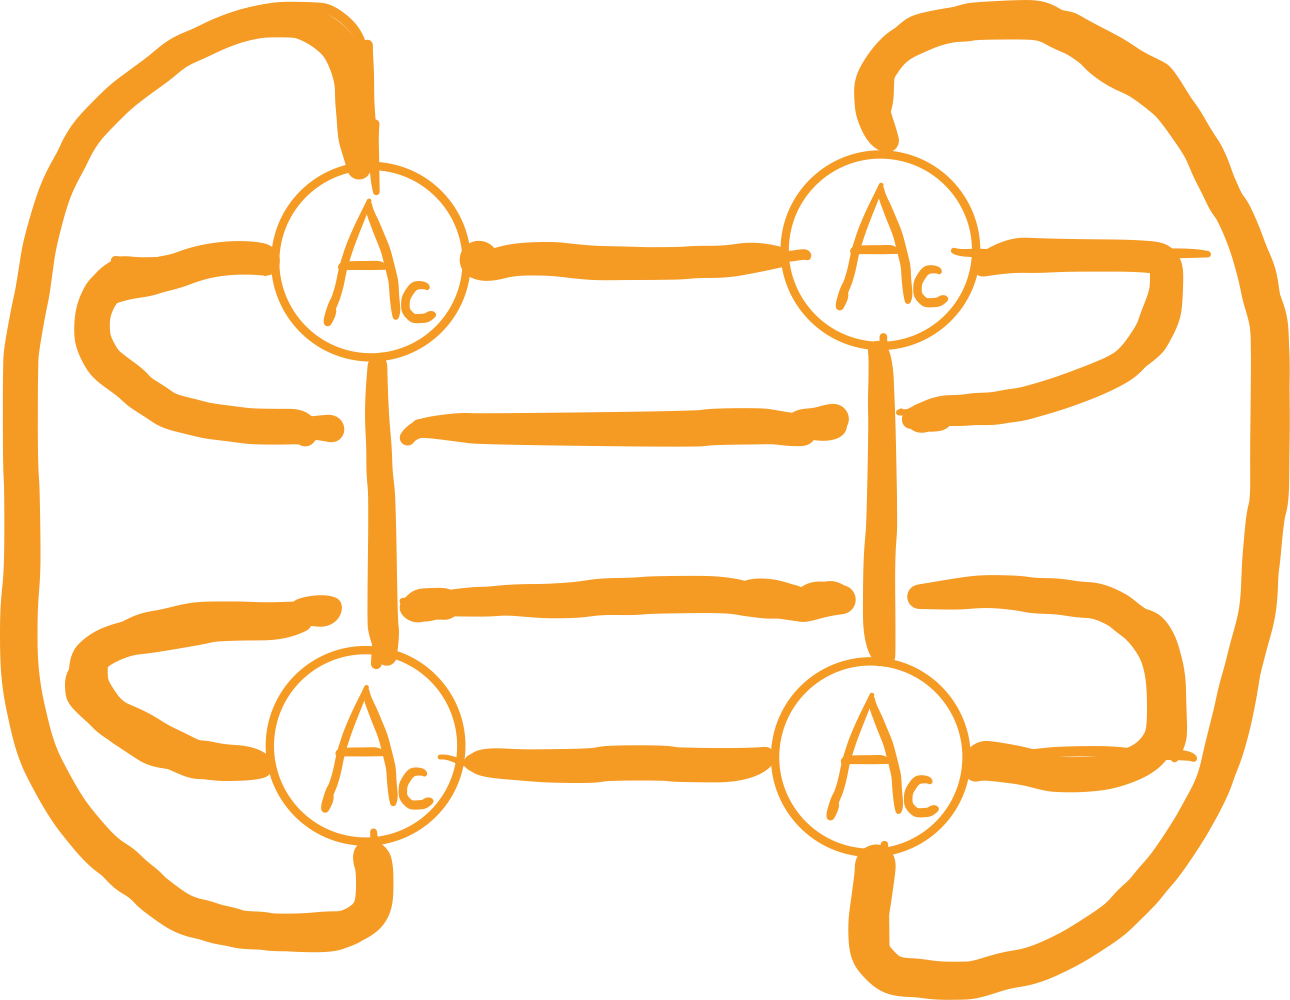
\includegraphics[width=2.6truecm,clip]{./figs/Z-underRG}
    \end{minipage}.
\end{align}
%
It is also enlightening to put the original spin variables back into the
tensor network to get a more physical picture of what is happening under
such tensor block RG transformation. To avoid too many lines clustering
together, we only keep spin variables, tensors and black solid squares
in Fig.~\ref{fig:spin2tensor}. The big picture for the above coarse
graining process is shown schematically in Fig.~\ref{fig:rgschem} below.
%
\begin{figure}[h]
    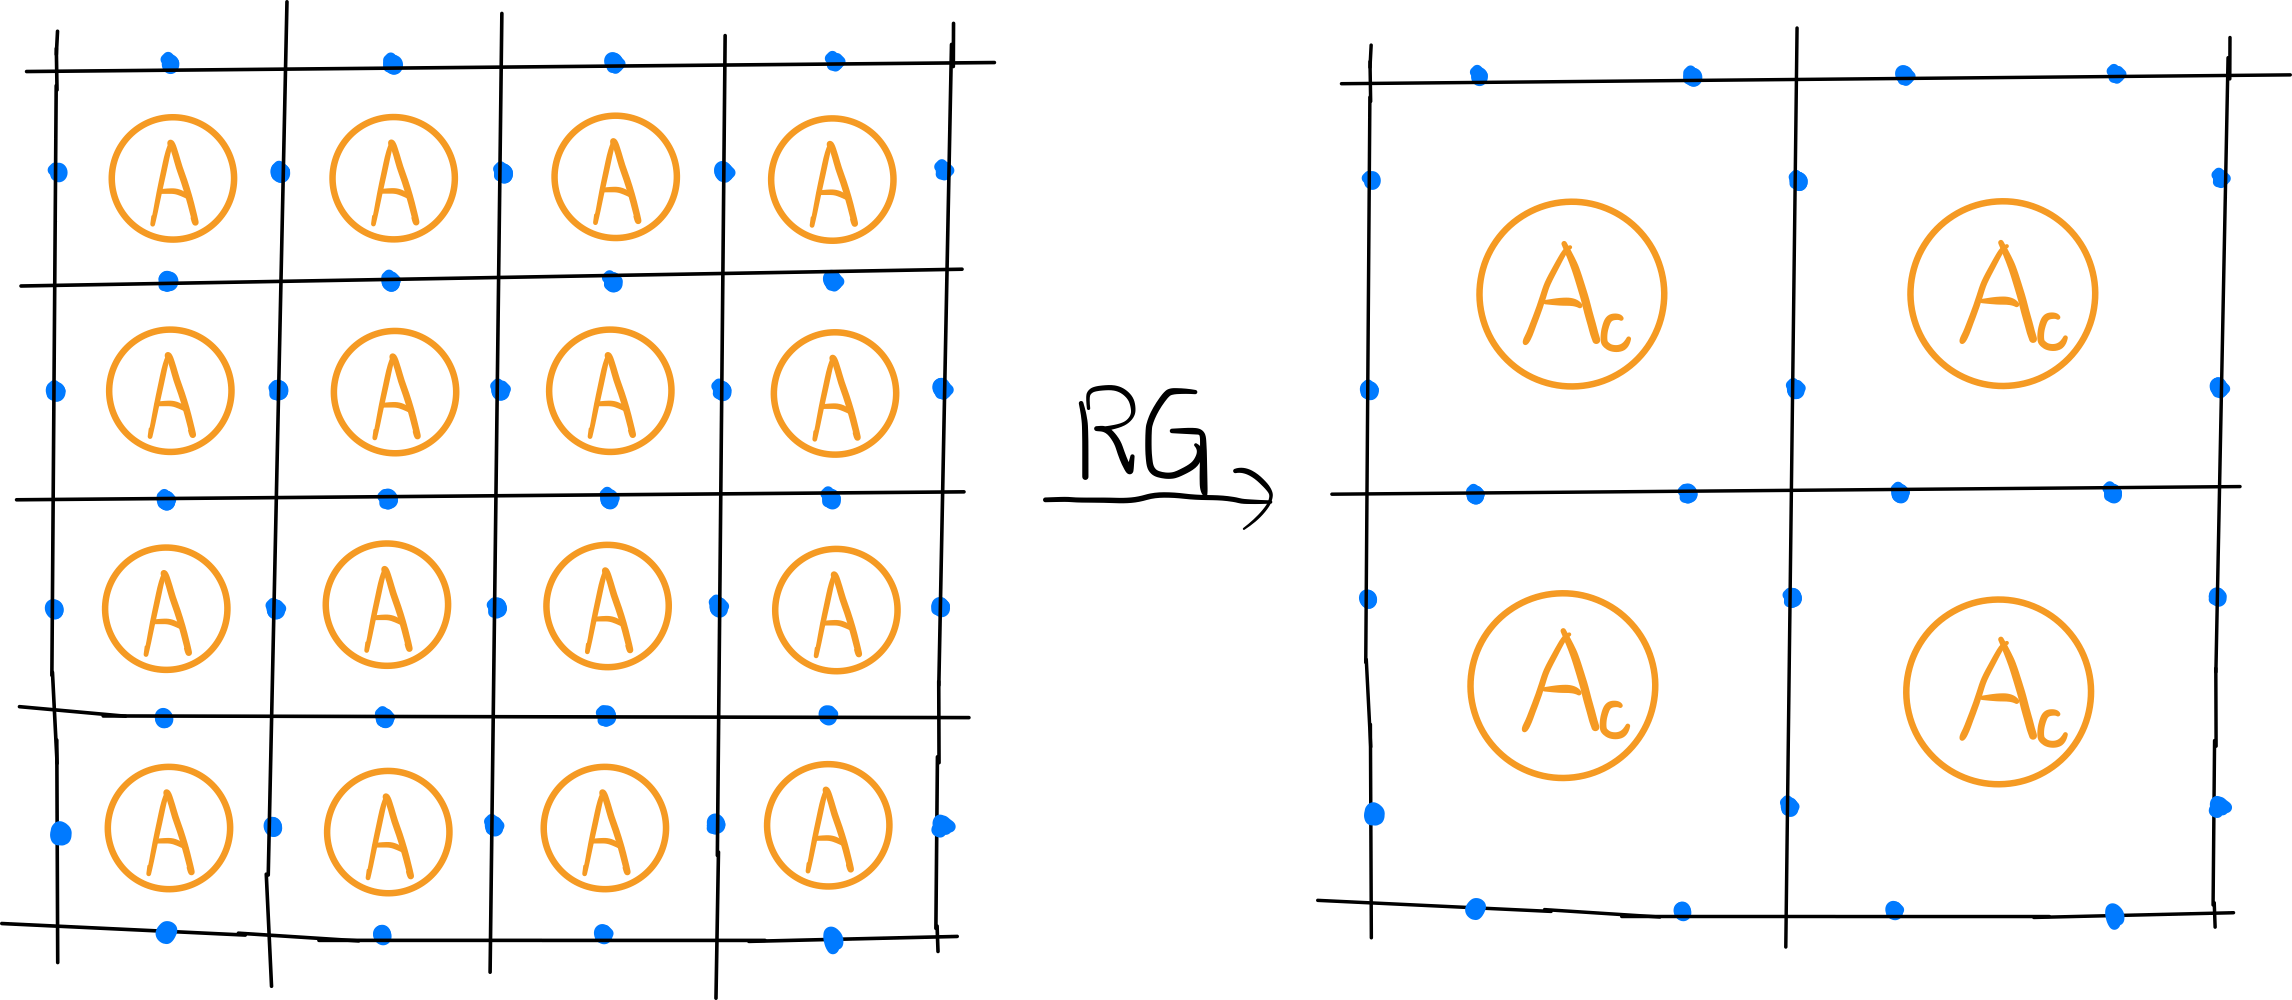
\includegraphics[width=8.5cm]{./figs/rgschem}
    \caption{\label{fig:rgschem}[\textbf{Add descriptions}]}
\end{figure}
%
The process is similar to decimation in the conventional approach. After
the spin variables shared by two tensors are summed over, we are left
with four bigger black squares, with two spin variables sitting on each
side of each square. The length scale is multiplied by $b = 2$. The RG
equation is then defined as a mapping from the old tensor $A$ to the new
tensor $A_c$ after coarse graining,
%
\begin{align}\label{eq:RGeqExact}
    \begin{minipage}{2.0truecm}
        \centering
        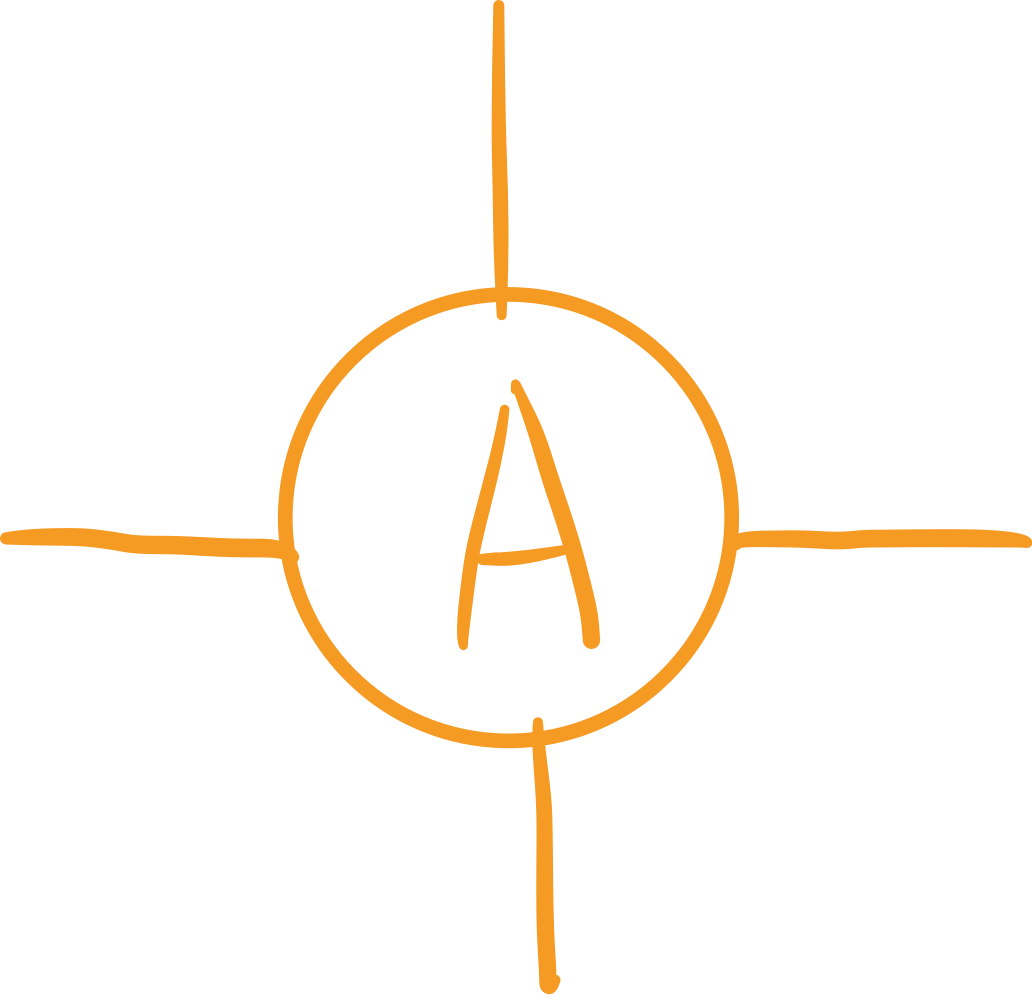
\includegraphics[width=1.8truecm,clip]{./figs/Aold}
    \end{minipage}
    \xrightarrow{\text{RG}}
    \begin{minipage}{2.0truecm}
        \centering
        
\includegraphics[width=1.8truecm,clip]{./figs/Ac-thickleg}
    \end{minipage}. 
\end{align}
%
%
The coarse graining scheme above is exact, but the bound dimension grows
fast. The initial tensor has bound dimension $\chi = 2$. After $n$ RG
transformations, the bound dimension grows to $2^{2^n}$. It can be
easily shown that the computation cost will grow exponentially in the
original lattice size. A clever approximation technique is necessary to
prevent the bound dimension from growing as RG transformation goes.
%

In the conventional RG approach, we avoid generating a Hamiltonian with
infinitely many interaction terms by only keeping a finite number of the
couplings that important quantitatively~\cite{wilsonNobel,wilson1970a}.
This statement was confirmed by Wilson himself in his 1975 numerical RG
calculations of 2D Ising model using Kadanoff's decimation
approach~\cite{wilsonNumRG}. This observation suggests that we should be
able to find a good approximation of a local patch of tensors, such as the
square of four $A$ tensors in Eq.~\eqref{eq:exactBlock}. We will
introduce such an approximation scheme, HOTRG, in the next subsection.


\subsection{HOTRG\label{hotrg}}
HOTRG~\cite{hotrg} is the earliest TRG-type technique that can be easily
applied on 3D classical lattice models. Since the method of extracting
scaling dimensions by analyzing the RG transformation around a critical
fixed point tensor has the advantange in 3D and higher, we want to
perform the numerical calculation in a such a way that generalization to
3D and higher is straightforward. HOTRG is a nice choice for our
purpose. It is simple to implement and has a beautiful pictorial
representation for the response analysis where we linearize the RG
equation near a critical fixed point tensor, as will be shown in
Sec.~\ref{diffRGeq}.
%

As is explained in the end of previous subsection, we want to
approximate the square of four $A$ tensors in the right hand side of
Eq.~\eqref{eq:exactBlock} in order to prevent the growing of bound
dimension. In the original treatment~\cite{hotrg}, the approximation was
explained in terms of higher-order singular value
decompositions~\cite{hosvd1,hosvd2,hosvd3}.  However, we will present
HOTRG from a different perspective inspired by a broader class of local
approximation methods called projective truncations\cite{tnr}. Let's
imagine we first contract two left $A$ tensors in
Eq.~\eqref{eq:exactBlock}. A projection operator $P = w w^{\dagger}$ is
inserted and acts on, say, two left legs whose bound dimenions are both
assumed to be $\chi$, and we hope this patch of two $A$ tensors after
projection gives a good approximation to the original patch,
%
\begin{align}\label{eq:hotrgProjTrun}
    \begin{minipage}{2.8truecm}
        \centering
        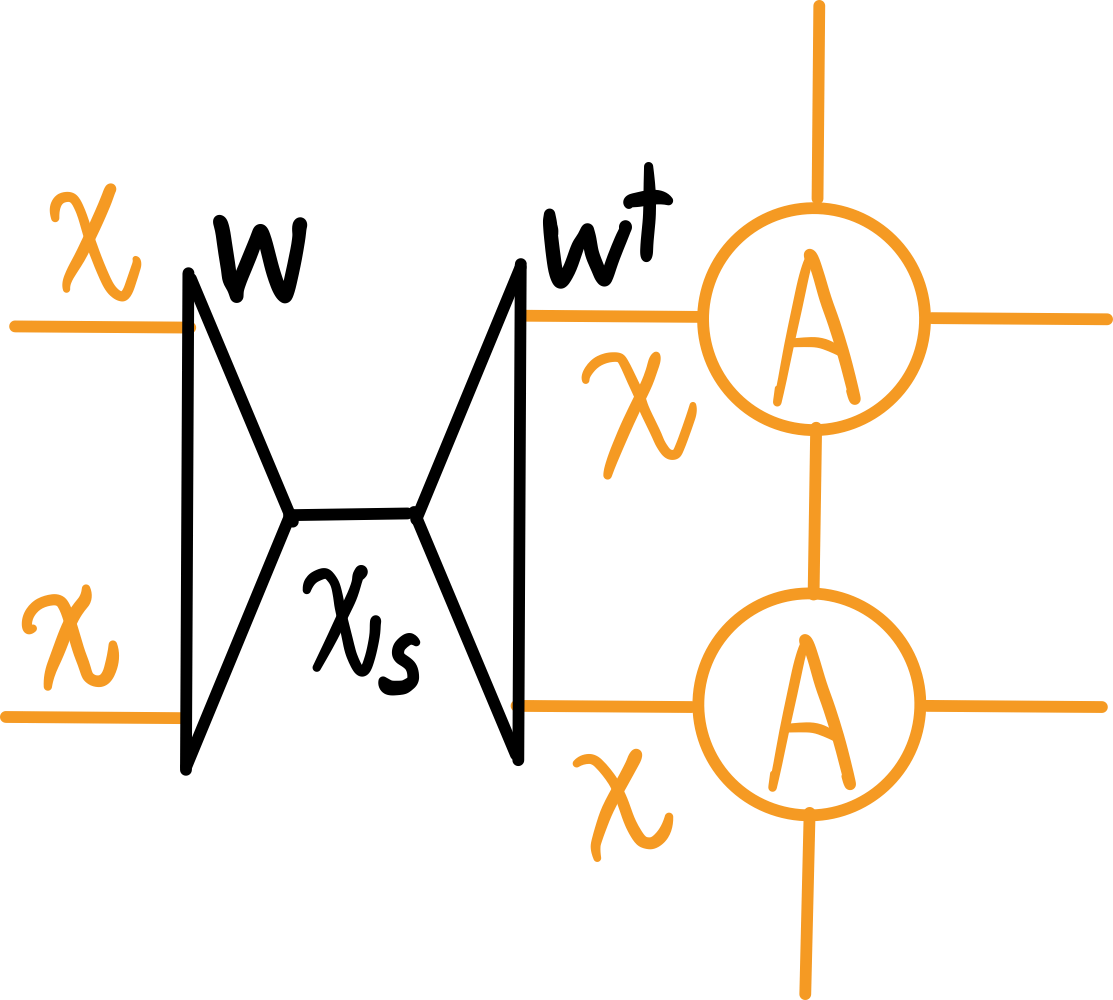
\includegraphics[width=2.6truecm,clip]{./figs/twoAProj}
    \end{minipage}
    \approx
    \begin{minipage}{1.6truecm}
        \centering
        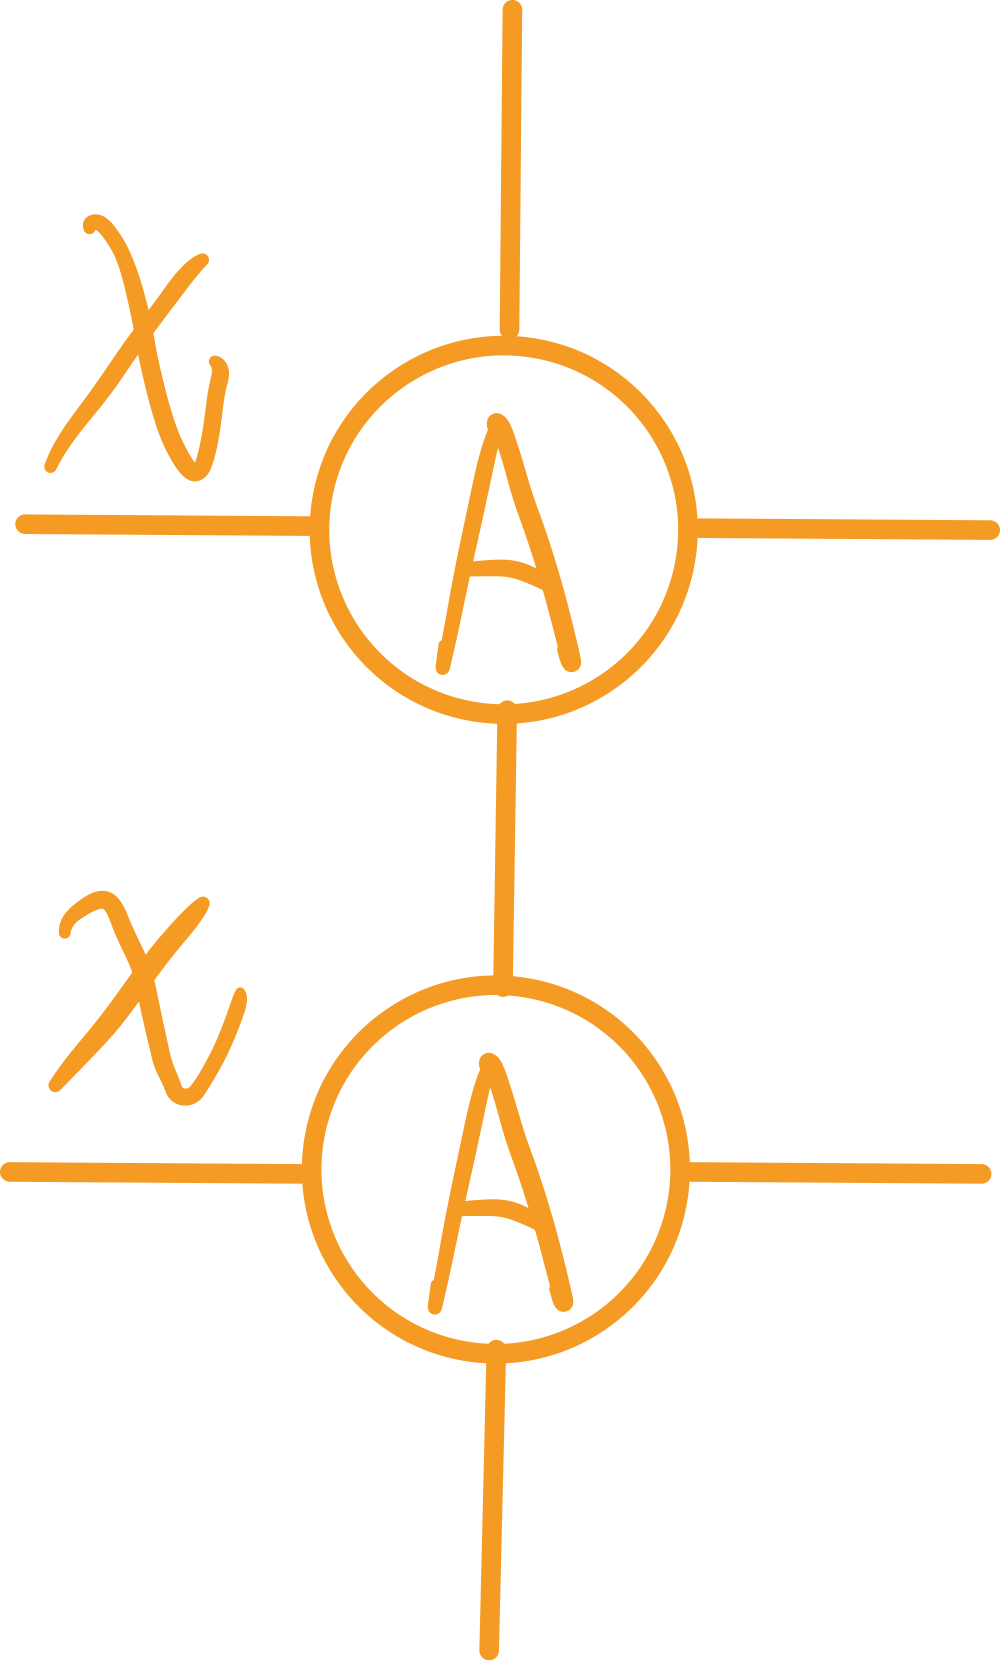
\includegraphics[width=1.4truecm,clip]{./figs/twoA}
    \end{minipage}.
\end{align}
%
Here, $w$ is an isometric tensor and $w^{\dagger}$ its hermitian
conjugate (or transpose if $w$ is a real tensor). The isometry is a
linear mapping:
$\mathbb{V}_{\chi}\otimes\mathbb{V}_{\chi}\rightarrow\mathbb{V}_{\tilde{\chi}}$,
where $\mathbb{V}_{\chi}$ denotes a $\chi$-dimensional vector space, and
it satisfies $w^{\dagger}w = \mathbb{1}$. In a more physicists-oriented
language, the isometry $w$ is nothing but a collection of $\tilde{\chi}$
orthonormal ket vectors with dimensionality $\chi^2$ in a given
representation. In fact, we draw it as a black triangle to mimic Dirac's
bra-ket notation. If we fix the leg connecting the vertex angle of
the black triangle to be $k$-th index, we get a ket vector $\ket{w_k}$.
The projection operator is $P =
\sum_{k=1}^{\tilde{\chi}}\ket{w_k}\bra{w_k}$. If $\tilde{\chi} =
\chi^2$, we have a complete orthonormal set and the projection operator
becomes the identity operator. We will see later that in order to
prevent the growing of the bound dimension, we should choose
$\tilde{\chi} \leq \chi$.
%

Now, suppose we have found the isometry $w$ that gives a good approximation
in Eq.~\eqref{eq:hotrgProjTrun}, then we use this approximation to
replace all pairs of $A$ tensors in the tensor network represention of
the partition function in Eq.~\eqref{eq:tensorZ4by4} to get
%
\begin{align}\label{eq:Zapproxy}
    Z_{4 \times 4}
    &\textapprox{\eqref{eq:hotrgProjTrun}}
    \begin{minipage}{3.2truecm}
        \centering
        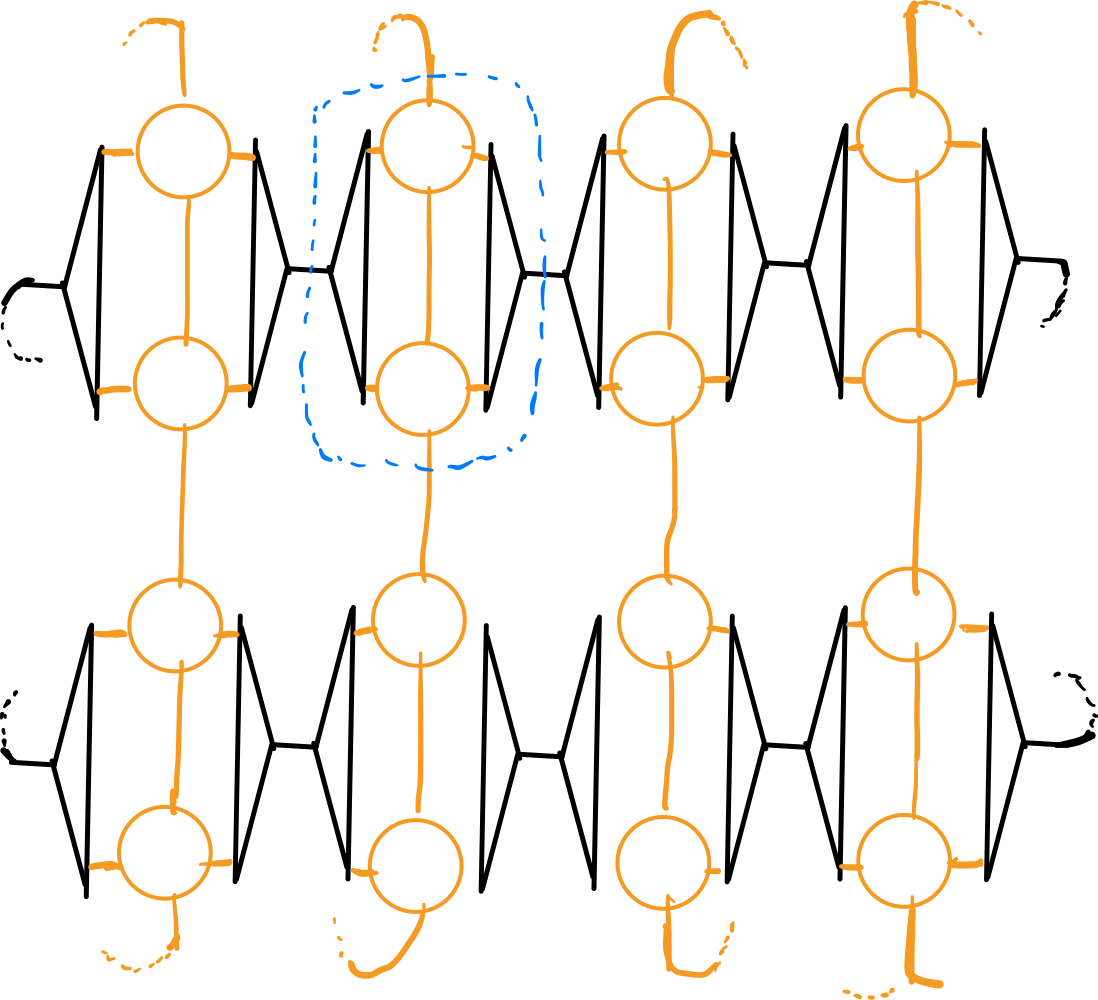
\includegraphics[width=3.0truecm,clip]{./figs/Z-approy}
    \end{minipage} \nonumber\\
    &=
    \begin{minipage}{3.5truecm}
        \centering
        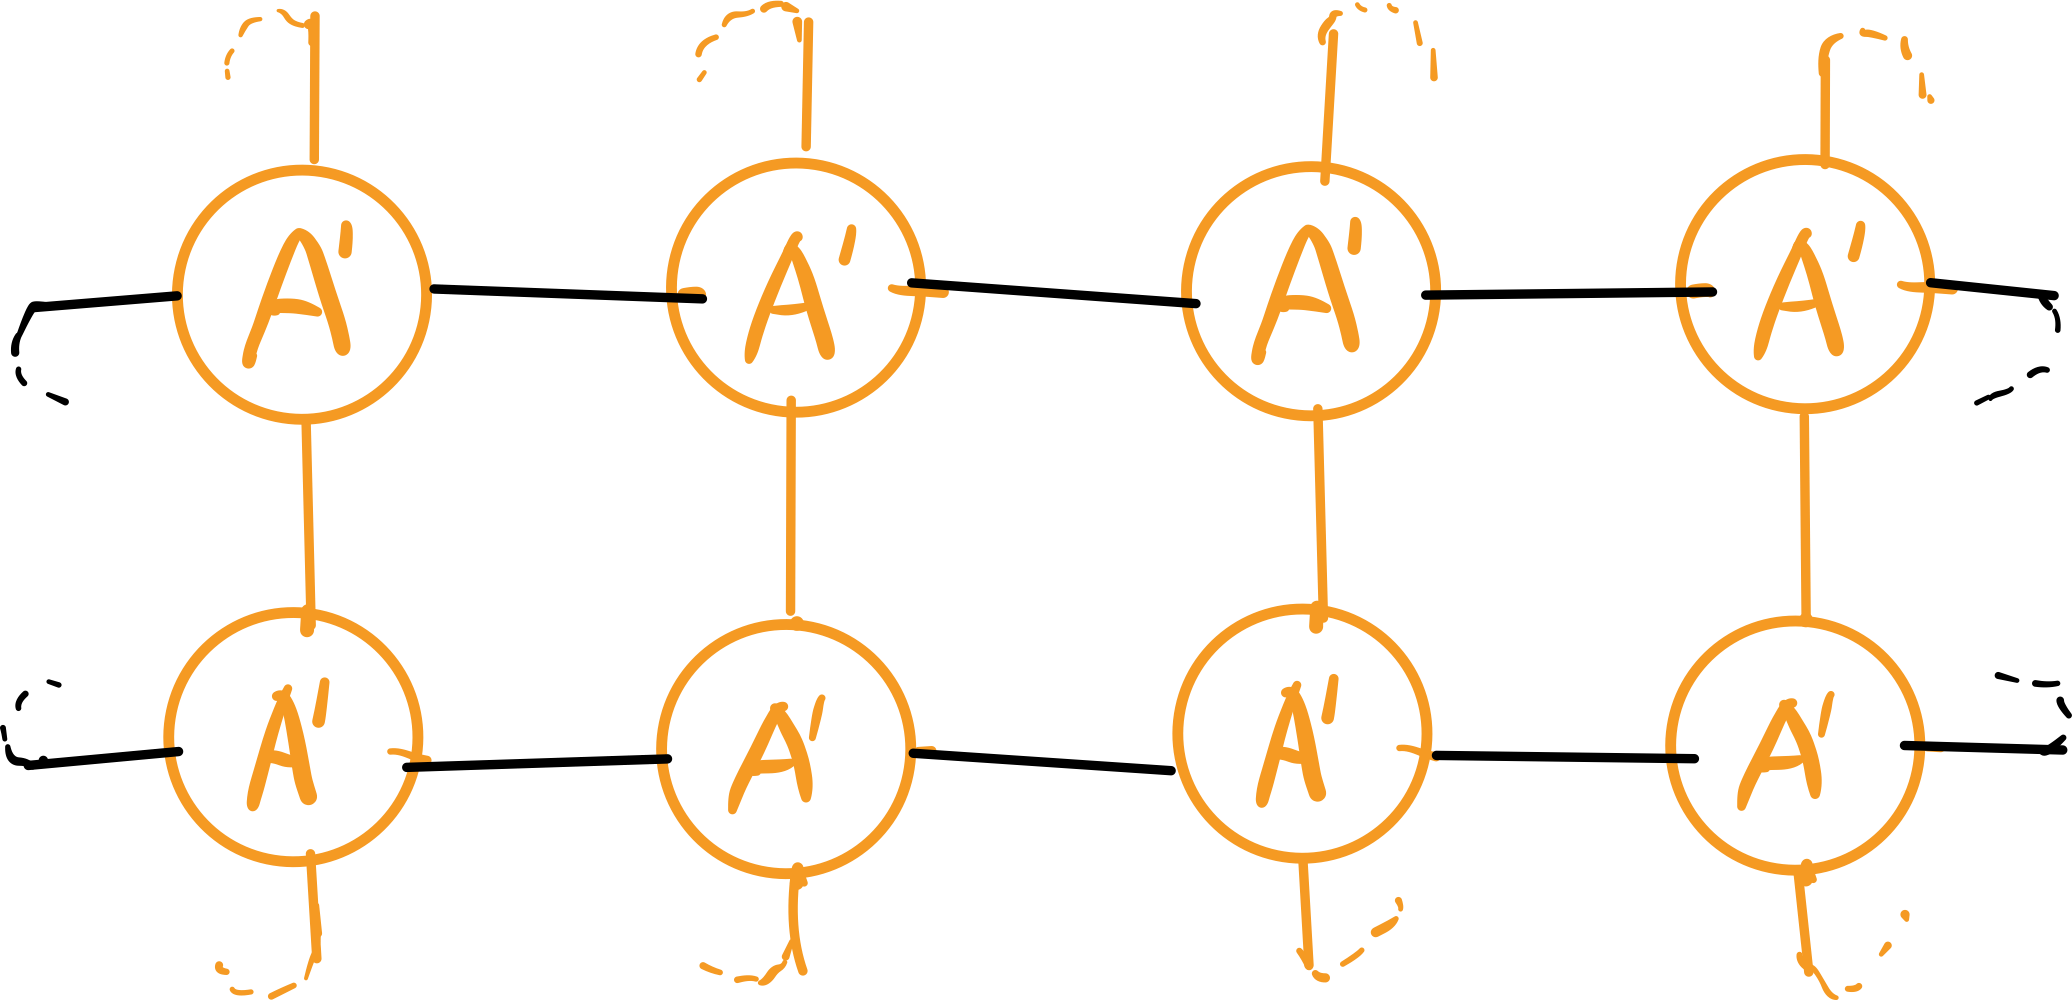
\includegraphics[width=3.3truecm,clip]{./figs/Z-contry}
    \end{minipage},
\end{align}
%
where in the second step, we contract two $A$ tensors and two isometric
tensors $w, w^{\dagger}$ to get a new tensor $A'$,
%
\begin{align}\label{def:Apycontr}
    \begin{minipage}{2.0truecm}
      \centering
      
\includegraphics[width=1.8truecm,clip]{./figs/Ap-ycontr}
    \end{minipage}
    \defeq
    \begin{minipage}{2.0truecm}
      \centering
      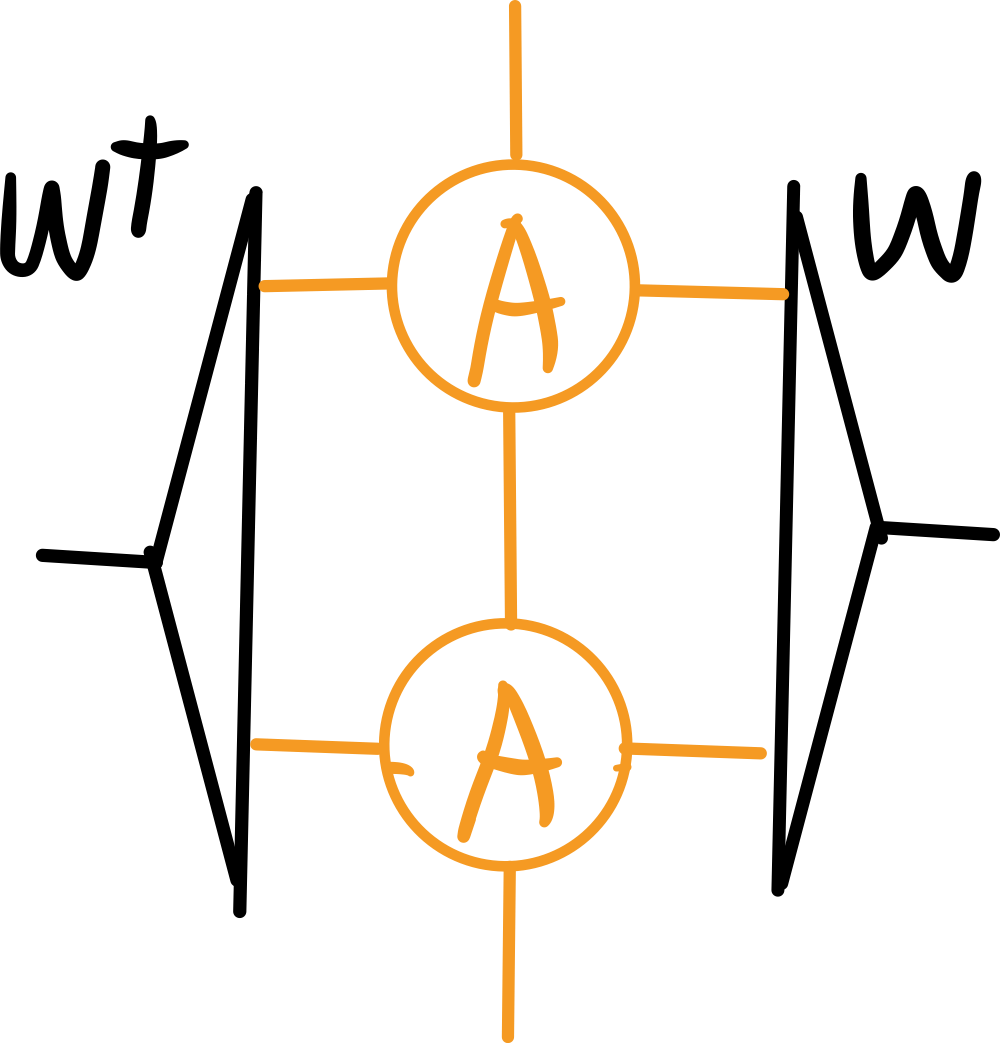
\includegraphics[width=1.8truecm,clip]{./figs/twoAcoarse}
    \end{minipage}.
\end{align}
%
Notice in the approximatino step in Eq.~\eqref{eq:Zapproxy}, we can move
two leftmost $w$ tensors to the far right because we have a periodic
boundary condition. Equation~\eqref{def:Apycontr} defines a coarse
graining process $A \rightarrow A'$ in the vertical direction. 
%

Apply a similar projective trunction on two $A'$ tensors put side by
side using another isometry $v$, we will get a coarse graining $A'
\rightarrow A_c$ in the horizontal direction,
%
\begin{align}\label{def:Achotrg}
    \begin{minipage}{2.0truecm}
      \centering
      
\includegraphics[width=1.8truecm,clip]{./figs/Ac-hotrg}
    \end{minipage}
    \defeq
    \begin{minipage}{2.0truecm}
      \centering
      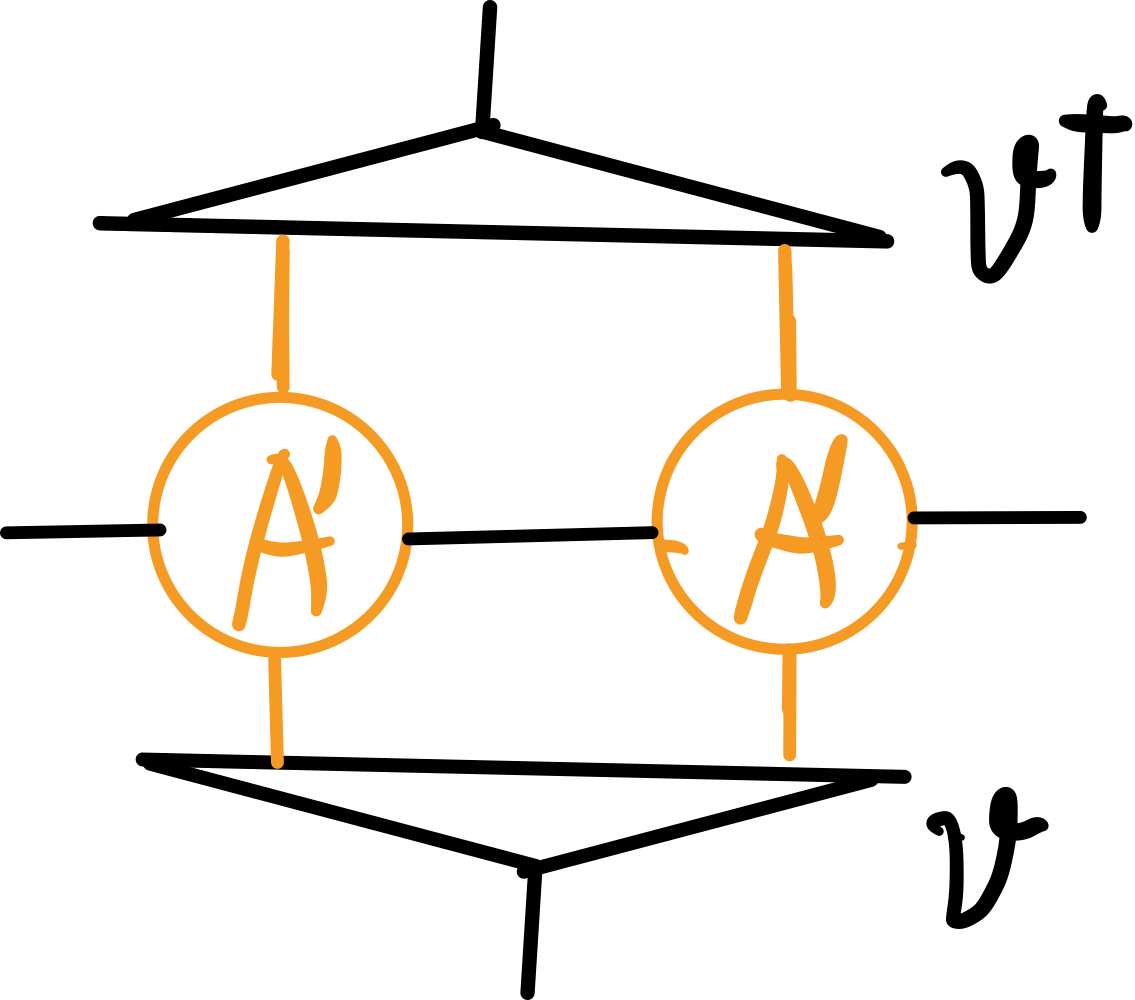
\includegraphics[width=1.8truecm,clip]{./figs/twoApcoarse}
    \end{minipage}.
\end{align}
%
Equation~\eqref{def:Apycontr} and~\eqref{def:Achotrg} combined together
defines an RG transformation
%
\begin{subequations}\label{def:RGeqHOTRG}
    \begin{align}\label{def:RGeqHOTRGschem}
    \begin{minipage}{2.0truecm}
        \centering
        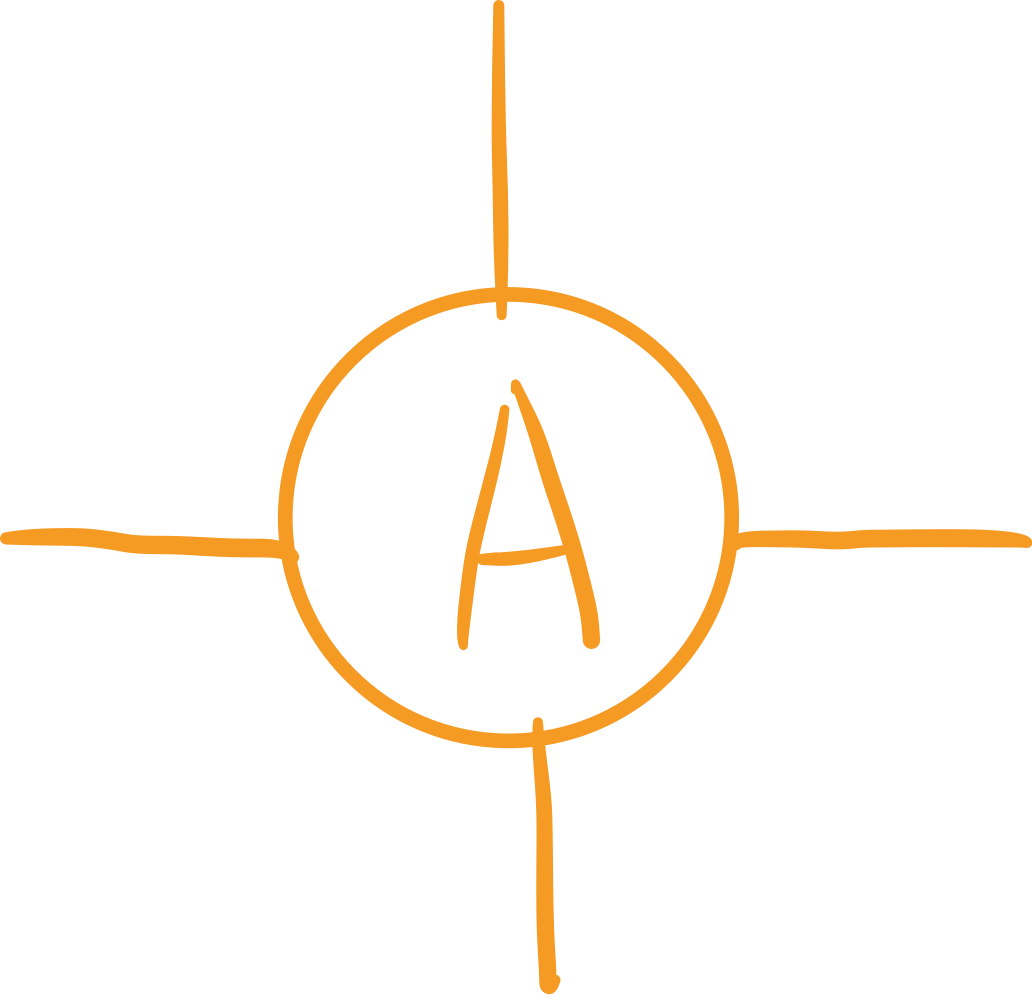
\includegraphics[width=1.8truecm,clip]{./figs/Aold}
    \end{minipage}
    \xrightarrow{\text{HOTRG}}
    \begin{minipage}{2.0truecm}
        \centering
        
\includegraphics[width=1.8truecm,clip]{./figs/Ac-hotrg}
    \end{minipage},
    \end{align}
or explicitly as
    \begin{align}\label{def:RGeqHOTRGepl}
    \begin{minipage}{2.0truecm}
        \centering
        
\includegraphics[width=1.8truecm,clip]{./figs/Ac-hotrg}
    \end{minipage}
    = 
    \begin{minipage}{4.0truecm}
        \centering
        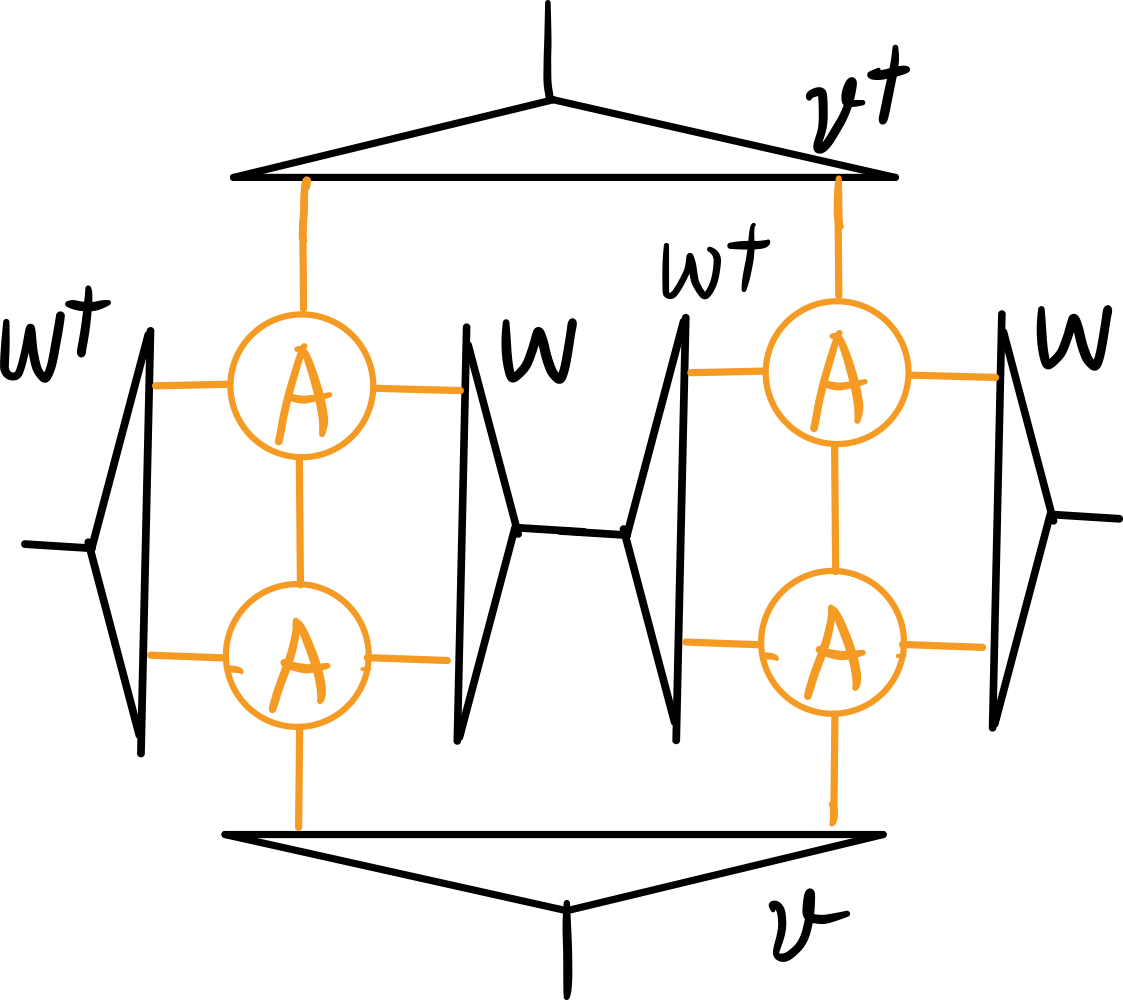
\includegraphics[width=3.8truecm,clip]{./figs/rgEq4HOTRG}
    \end{minipage}.
    \end{align}
\end{subequations}
%
The legs of tensor $A_c$ have the bound dimension $\tilde{\chi} \leq
\chi$, so HOTRG implements an approximate RG transformation which
prevents the bound dimension from growing.

The final question is how to determine the isometry $w$, so that we have
a good approximation in Eq.~\eqref{eq:hotrgProjTrun}. The approximation
error is usually quantified by the Frobenius norm of the difference of
two tensors. To simplify the notation, we combine two left legs of the
patch of two $A$ tensors in right hand side of
Eq.~\eqref{eq:hotrgProjTrun} as one group, and combine its remaining
four legs as the other group and treat it as a matrix $M$,
%
\begin{align}\label{def:M-AA}
    M = 
    \begin{minipage}{1.6truecm}
        \centering
        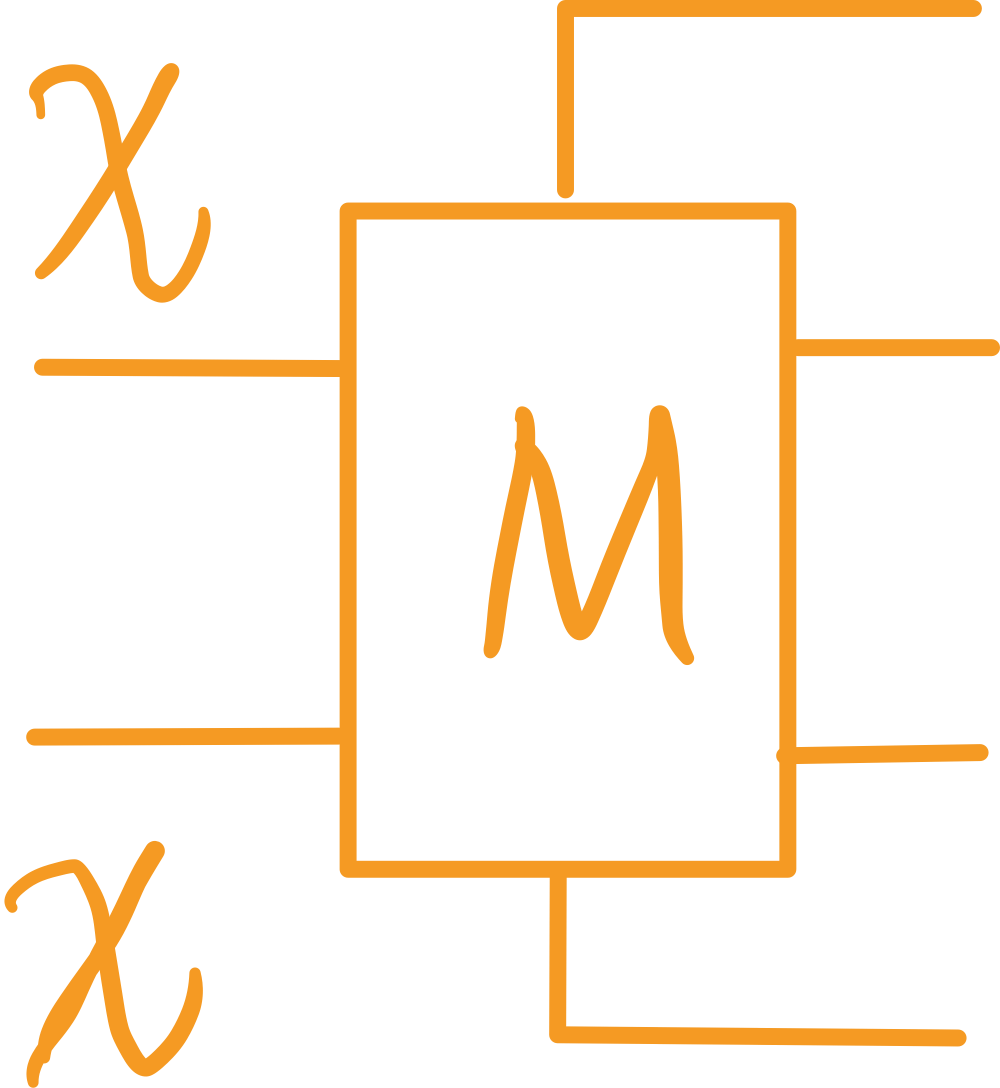
\includegraphics[width=1.4truecm,clip]{./figs/M-AA}
    \end{minipage}
    \defeq
    \begin{minipage}{1.6truecm}
        \centering
        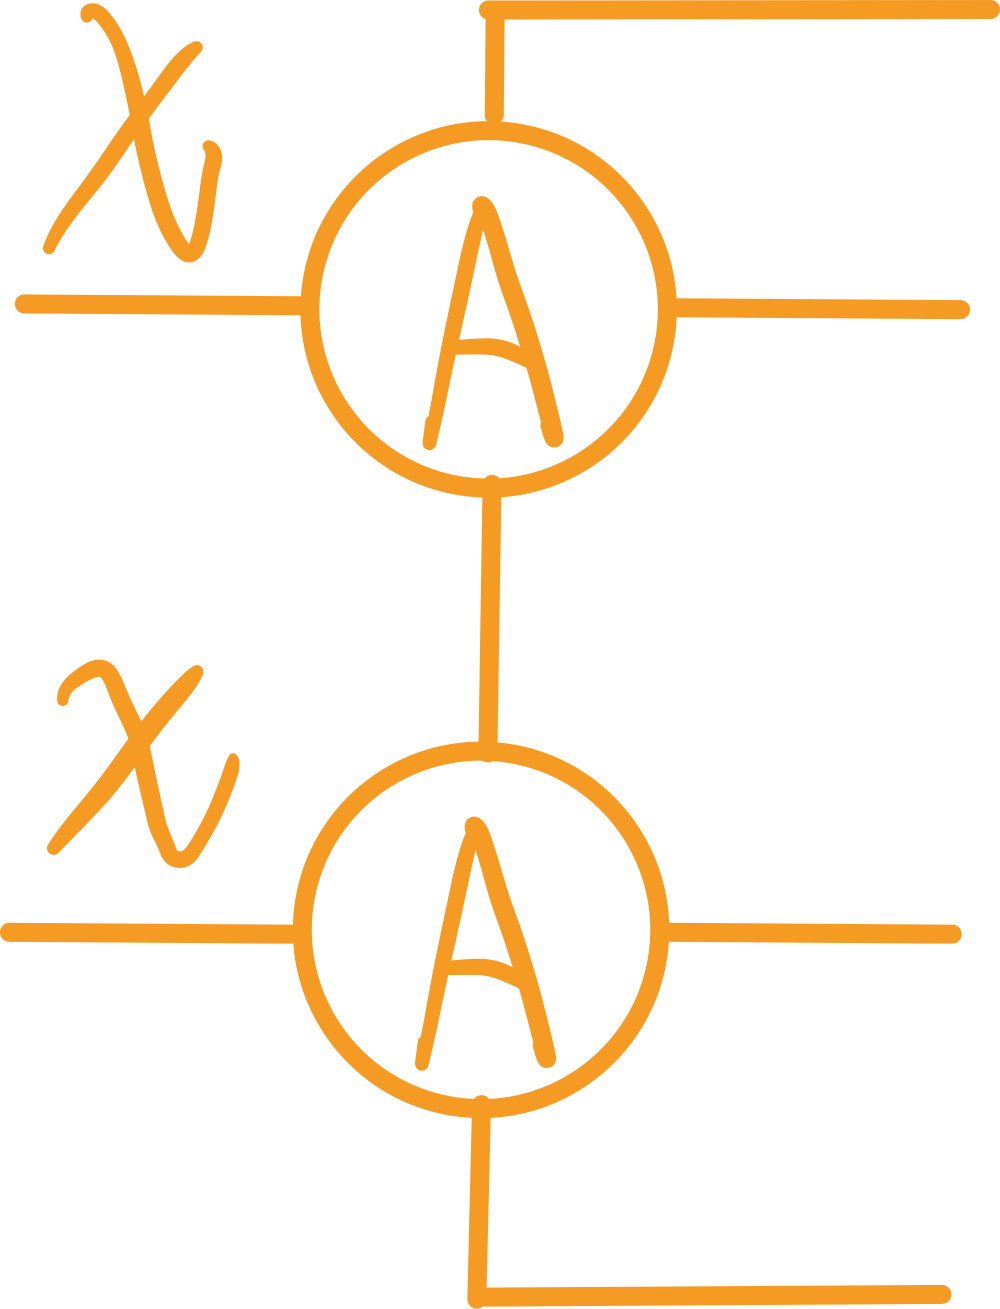
\includegraphics[width=1.4truecm,clip]{./figs/twoA2M}
    \end{minipage}.
\end{align}
%
The square of the approximation error $\epsilon$ of
Eq.~\eqref{eq:hotrgProjTrun} is
%
\begin{subequations}\label{eq:approxerrAll}
    \begin{align}\label{eq:approxerr}
    \epsilon^2 &= \left\Vert M - w w^{\dagger}M \right\Vert_{F}^{2}
    \nonumber \\ 
    &= \Tr\left(\left(M - w w^{\dagger}M \right) \left(M -
    ww^{\dagger}M\right)^{\dagger}  \right ) \nonumber\\
    &= \Tr\left(M M^{\dagger}\right) - \Tr\left(w^{\dagger}M
    M^{\dagger}w\right),
    \end{align}
where in the last step, we expand the two brackets, apply the cyclic
property of trace, and use the property of an isometry, $w^{\dagger}w =
\mathbb{1}$. Notice the first term $\Tr\left(M M^{\dagger}\right)$ is
a constant since matrix $M$ is given. The result can be put pictorially
as 
%
    \begin{align}\label{eq:approxerrPic}
    \epsilon^2 = \text{Const.} - 
    \begin{minipage}{4.2truecm}
        \centering
        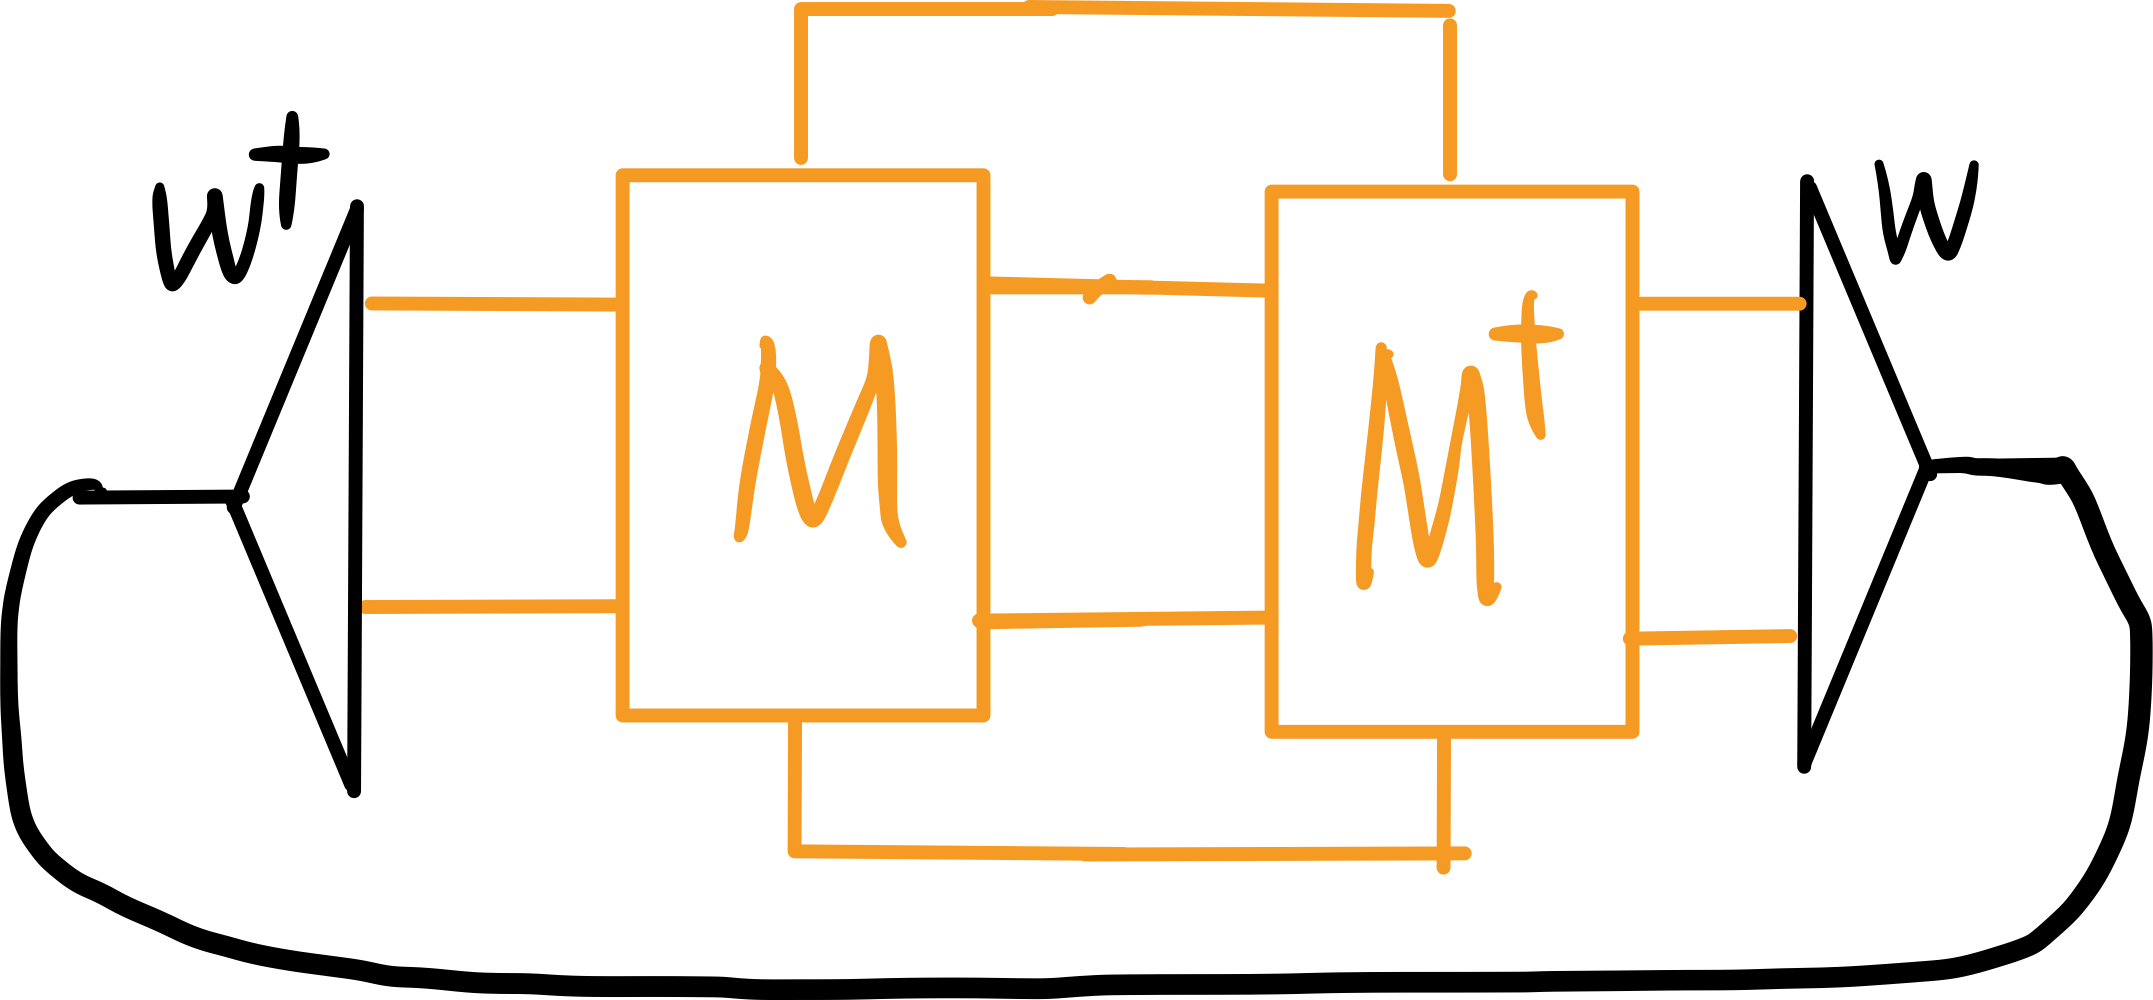
\includegraphics[width=4.0truecm,clip]{./figs/wMMw}
    \end{minipage}.
    \end{align}
\end{subequations}
%
Since the sqaure of any number is non-negative, we have $\Tr\left(
w^{\dagger}M M^{\dagger} w\right) \leq \Tr\left(M M^{\dagger}\right)$.
It follows that $\epsilon$ in Eq.~\eqref{eq:approxerrAll} is minimized
when $\Tr\left(w^{\dagger}M M^{\dagger}w\right)$ is maximized. It is a
well-known optimization problem that can be converted into an eigenvalue
problem~\cite{ghojogh2019eigenvalue}. In Appendix~\ref{appd:opteig}, we
will use the method of Lagrangian multiplier to prove this statement.
The optimal isometry $w$ is a collection of $\tilde{\chi}$ eigenvectors
of the positive semi-definite matrix $M M^{\dagger}$ with the first
$\tilde{\chi}$ largest eigenvalues. For example, the ket vector
$\ket{w_k}$ corresponding to the column vector we get when fixing the
leg connecting the vertex angle of $w$ (see, for example, the figure in
Eq.~\eqref{eq:approxerrPic}) should satisfy 
%
\begin{align}\label{eq:optwCondi}
    M M^{\dagger}\ket{w_k} = \lambda_k \ket{w_k},     
\end{align}
%
where $\lambda_k$ is the $k$-th largest eignvalues of $M M^{\dagger}$.
The sqaure of the approximation error $\epsilon^2$ in
Eq.~\eqref{eq:approxerrAll} is the sum of $\chi^2 - \tilde{\chi}$
smallest eigenvalues we throw away during the approximation.
%

In summary, instead of grouping two legs in Eq.~\eqref{eq:exactBlock}
directly, HOTRG performs a change of basis using the isometry $w$
defined in Eq.~\eqref{eq:optwCondi}. The importance of the new basis
vector $\ket{w_k}$ is reflected by the corresponding eigenvalues
$\lambda_k$.  $\tilde{\chi}$ most important state vector is choisen to
construct the isometry $w$. Perform the coarse graining of tensor $A$ in
the vertical direction according to Eq.~\eqref{def:Apycontr} to get
$A'$. Then, construct the isometry $v$ in the similar manner and perform
the corase graining of tensor $A'$ in the horizontal direction according
to Eq.~\eqref{def:Achotrg} to get $A_c$. The composite transformation
from $A$ to $A_c$ is the RG equation of HOTRG in
Eq.~\eqref{def:RGeqHOTRG}.
%

We hope the RG equation of HOTRG will exhibit critical fixed-point
tensors. However, the RG flow generated by the RG equation of HOTRG
suffers from the same problem as TRG. We will explain this problem and
introduce a way to solve it in the next section.


\section{RG Flow towards a fixed-point
tensor\label{fixRGflow}}
Most TRG-type techniques will give rise to a pecular RG flow of tensor,
HOTRG is no exception. Different points in the tensor space belonging to
the same phase do not flow to a single isolated fixed point. Instead,
they will flow to different points on a continuous fxied surface. Levin
anticipated this unconventional feature of TRG when looking for the
fixed-point tensors under TRG transformations~\cite{LevinTalk}. One of
the earlist numerical evidence for this peculiar RG flow of tensor for
2D Ising model by applying TRG was provided by Hinczewski and
Berker~\cite{Berker2008}. This indicates that TRG-type techniques fail
to integrate out all the local correlations at short distance, so physics at
lattice scale is carried all the way to the physics at larger length
scale. This shortcoming of TRG-type techniques makes identification of
both non-critical and critical fixed-point tesnors very difficult.
%

The local correlations can be understood quantitively by the
corner double-line (CDL) tensors. CDL tensors are fixed points of both
TRG~\cite{LevinTalk,GuWen2009,tnr,gilts} and HOTRG
transformations~\cite{hotrgfixpoint}.

In this section, we will explain CDL tensors and introduce a technique
called Graph-independent local truncation (Gilt)~\cite{gilts} to filter
out CDL tensors for HOTRG.

\subsection{Local correlations and CDL tensors\label{CDLten}}
To understand how local correlations at lattice scale arise in the
tensor network approach of RG, let us examine the physical picture of
the tensor block RG transformation in more detail. As is shown in
Fig.~\ref{fig:rgschem} in Sec.~\ref{spin2tensor}, tensor block RG
transformation erases inner edges of smaller black squares to build up
larger squares, with more spin variables located on its edges. HOTRG
simply express the states of the spin variables on each edges in another
basis determined by the isometries. When the black square becomes larger
enough, spin variables on different edges are far away from each other
and we expect they are uncorrelated. The only exception is for the spin
variables around the corner. See Fig.~\ref{fig:ariseCDL}. We can use a
matrix $C$ to capture such correlations around the corner and it must
contains physics at lattice scale. Since spin variables around different
corners are far away from each other, the tensor corresponding to this
black square should factorize into the tensor product of four corner
matrices $C$. A tensor with the structure of $A^{\text{CDL}}$ is called
a CDL tensor.
%
\begin{figure}[h]
    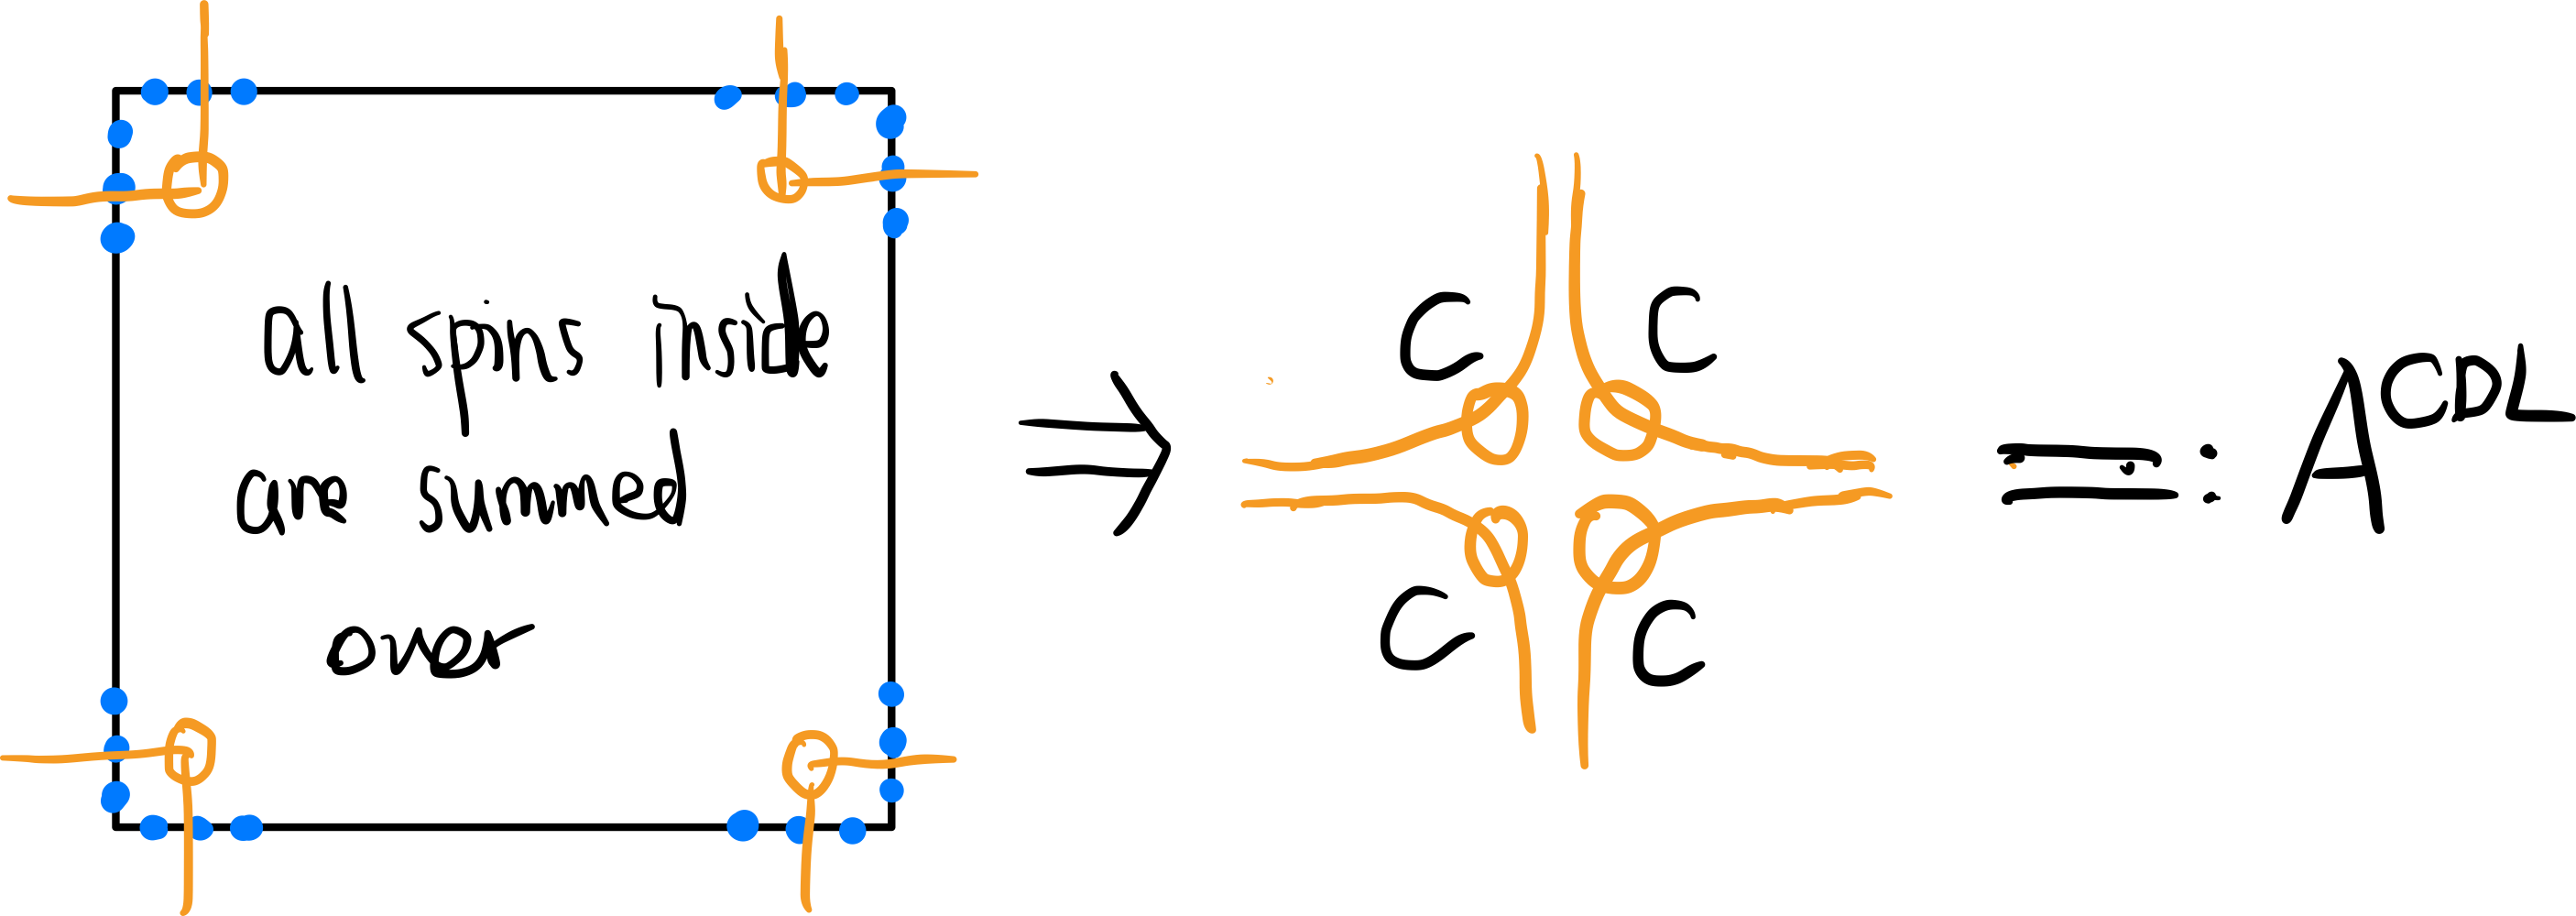
\includegraphics[width=7.5cm]{./figs/ariseCDL}
    \caption{\label{fig:ariseCDL}[\textbf{Add descriptions}]}
\end{figure}
%

We will explain in Appendix~\ref{appd:cdlHOTRG} that CDL tensors form a
class of fixed points for the RG equation of HOTRG in
Eq.~\eqref{def:RGeqHOTRGepl}. If we feed $A^{\text{CDL}}$ into the right
hand side of Eq.~\eqref{def:Apycontr}, the output tensor is propotional
to $A^{\text{CDL}}$,
%
\begin{align}\label{eq:cdlHOTRG}
    \begin{minipage}{4.0truecm}
        \centering
        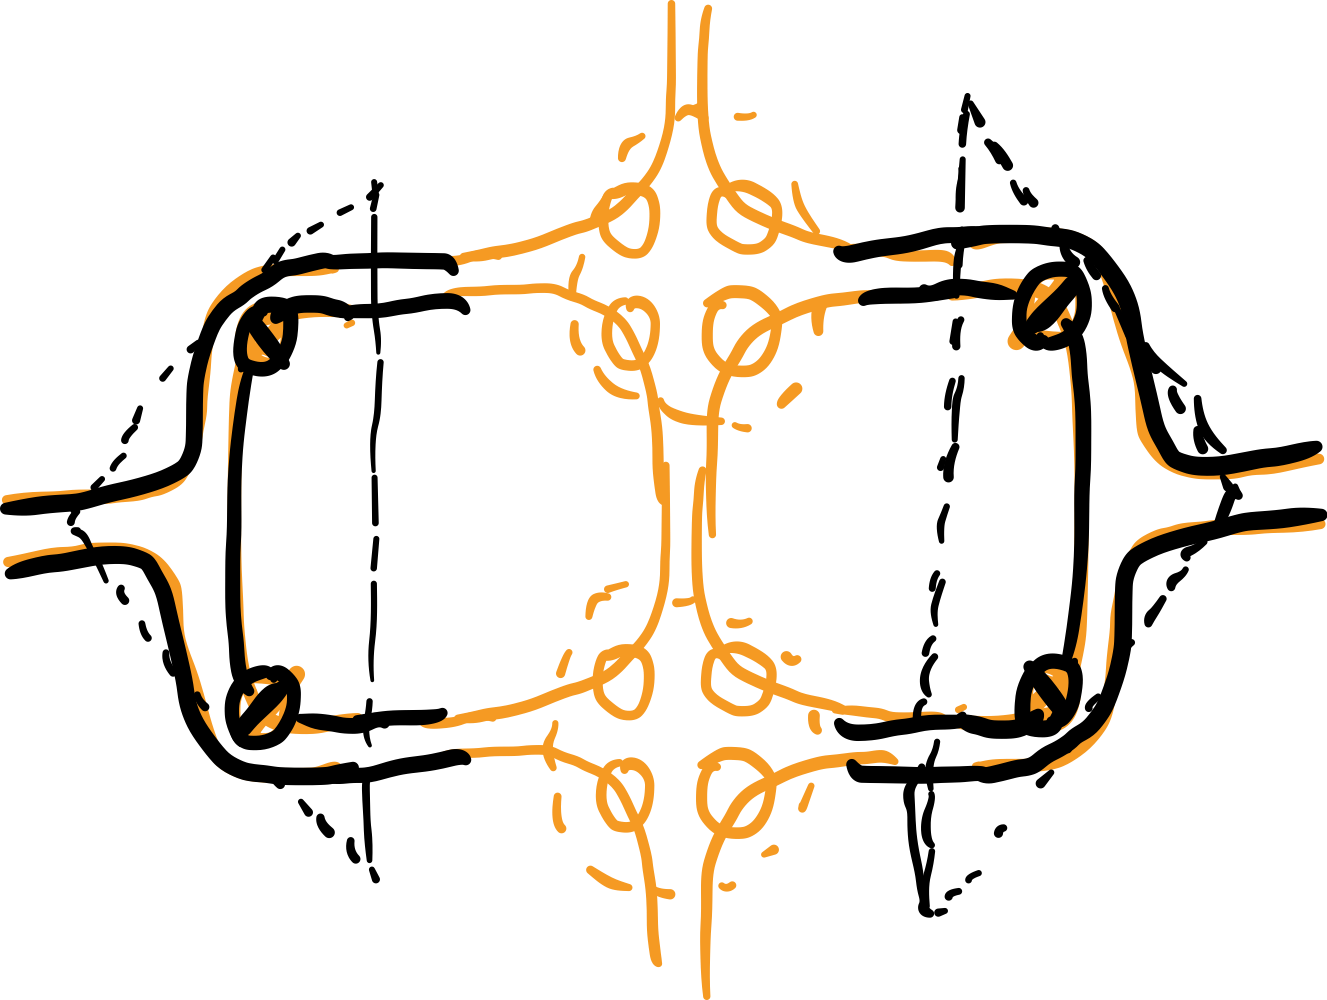
\includegraphics[width=3.8truecm,clip]{./figs/cdlHOTRG}
    \end{minipage}
    \propto
    \begin{minipage}{2.0truecm}
        \centering
        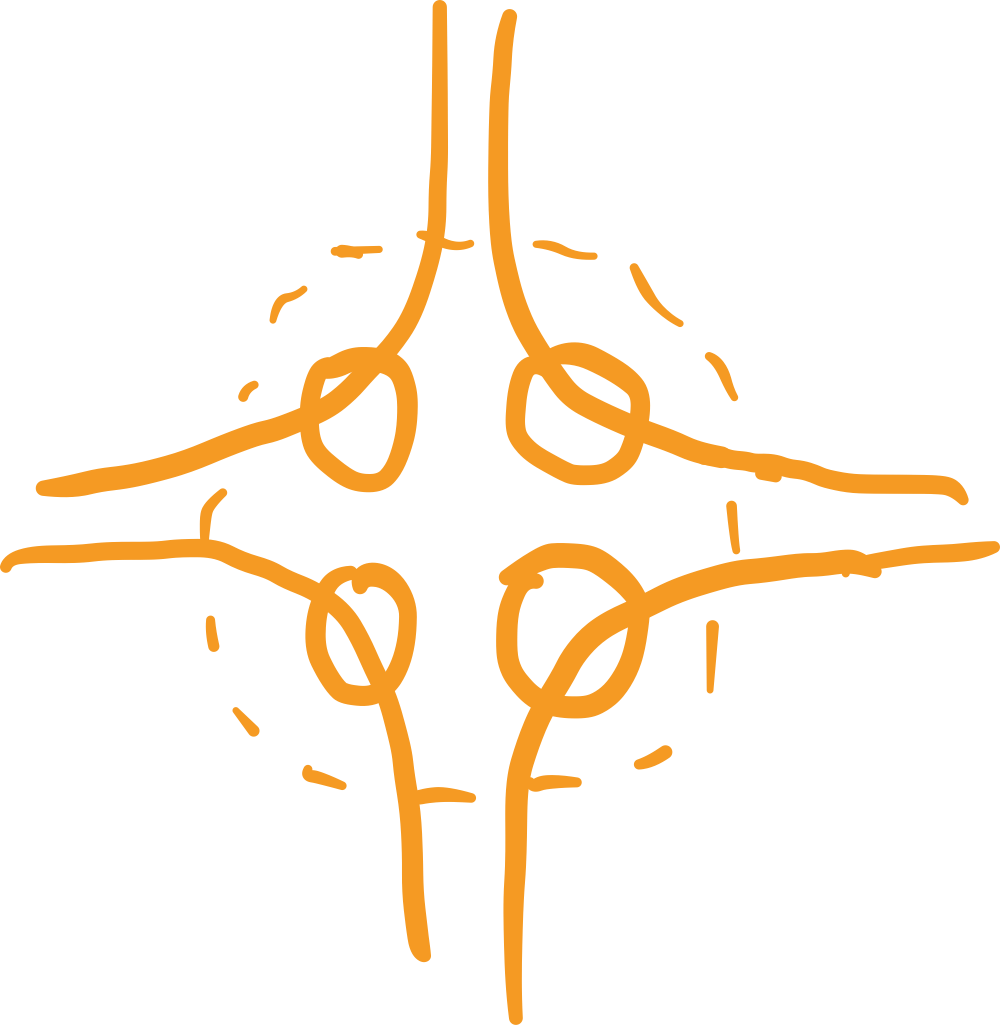
\includegraphics[width=1.8truecm,clip]{./figs/singleCDL}
    \end{minipage}.
\end{align}
%
Equation~\eqref{eq:cdlHOTRG} shows that although HOTRG can detect and
project out four inner C matrices, it can do nothing about the ourter
four C matrices. This means that HOTRG, like TRG, cannot integrate out
the local interactions among spin variables around the corners. If we
start with two temperatures $T_1 \neq T_2$ both larger than the critical
temperature of 2D Ising model $T_c$, HOTRG will generate tensors flow to
two different CDL tensors $A^{\text{CDL}}_1, A^{\text{CDL}}_2$. At
criticality, previous numcerical calculations indicate that we will
never reach a critical fixed-point tensor~\cite{Berker2008,tnr}. Their
calculations suggest a tensor RG flow shown in
Fig.~\ref{fig:tensorRGflow}(b), where the low and high temperature fixed
points turn into two fixed lines and the critical fixed point
disappears.
%
\begin{figure}[h]
    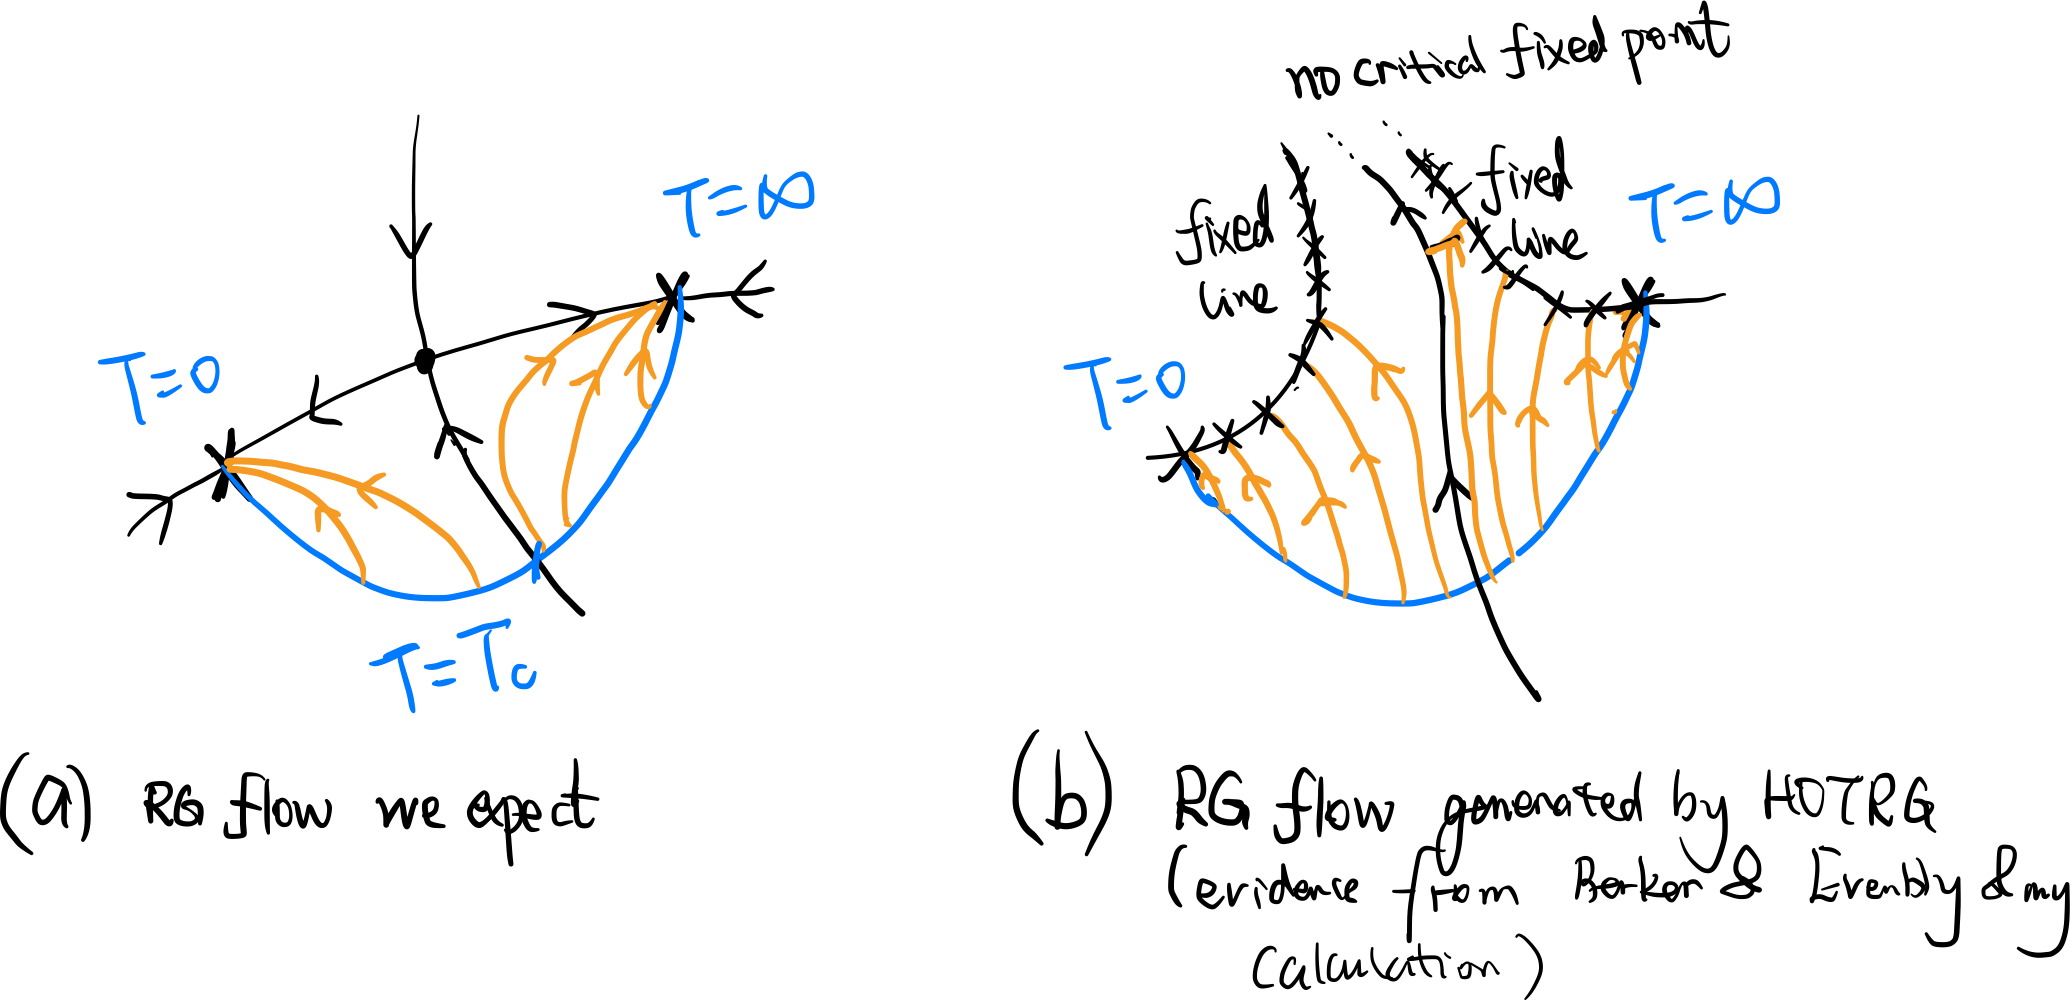
\includegraphics[width=8.6cm]{./figs/tensorRGflowSchem}
    \caption{\label{fig:tensorRGflow}[\textbf{Add descriptions}]}
\end{figure}
%

There are many ways to filter out the local correlations. Early attempts
include tensor-entanglement-filtering renormalization
(TEFR)~\cite{GuWen2009}, tensor network renormalization
(TNR)~\cite{tnr,tnralgo}, non-negative tensor network renormalization
(TNR+)~\cite{tnrplus} and loop-TNR~\cite{looptnr}. In these methods,
filtering of local correlations is mixed togehter with the ordinary
coarse graining procedure. They are powerful techniques in 2D, but
generalizations to 3D are complicated and usually come with very high
computational costs. 
%

In recent two years, several more convenient techniques appeared. They are
all stand-alone procedures to filer out or identify local correlations.
The main advantage is that they can in principle be combined with any
tensor coarse garining procedures. Harada~\cite{harada2018} proposed a
new operation called entanglemtn branching operator, designed to
manipuate the flow of local correlations in a tensor network. Lee and
Kawashima~\cite{tensor-ring} used an index-splitting strategy to
identify the exact inner structure of a given CDL tensor. Three quite
similar methods~\cite{tns,gilts,fet} focus on filtering the local
correlations by reducing bond dimensions in a tensor network without
changing its geometry. We choose one in these three methods,
Graph-independent local truncation (Gilt)~\cite{gilts}, to filter the local
correlations for HOTRG. It has be demonstrated that TRG combined with
Gilt will exhibit the critical fixed-point tensors of 2D Ising
model~\cite{gilts} and 2D $\phi^4$ theory~\cite{Delcamp2020}. We will
show in Sec.~\ref{benchmark} that HOTRG combined with Gilt can
successfully exhibit the critical fixed-point tensor for 2D Ising model.
However, let us first introduce Gilt and show how to intergrate it into
HOTRG.
%

\subsection{Gilt-HOTRG\label{gilt-hotrg}}
The key feature of Gilt is that it is stand-alone and does
not change the geometry of a given tensor network, so it is a very
flexible tool to use. Figure~\ref{fig:gilt} summarizes the process of
Gilt. The idea is the same as before when we perform the tensor coarse
graining transformation. Instead of finding an approximation of a patch
of two $A$ tensors in Eq.~\eqref{eq:hotrgProjTrun}, this time we want to
approximate a larger patch of four A tensors. The shading loop inside
the plaquette represents the local correlations consisting of four
corner matrices (see Fig.~\ref{fig:ariseCDL} and imagine put four CDL
tensors together to form a plaquette). The first step, which is the
most crucial one, is to insert a low-rank matrix $Q$ into the leg we
wish to truncate. We refer the reader to the original Gilt
paper~\cite{gilts} for how to find such a low-rank matrix. The remaining
two steps are exact and exact. We split $Q$ using SVD and absort it into
the adjacent two $A$ tensors. The bound dimension of the leg is smaller
and the local correlations on this leg are filtered out. We can repeat
the procedure on other three legs and filter out tehe local correlations
inside this plaquette completely.
%
\begin{figure}[h]
    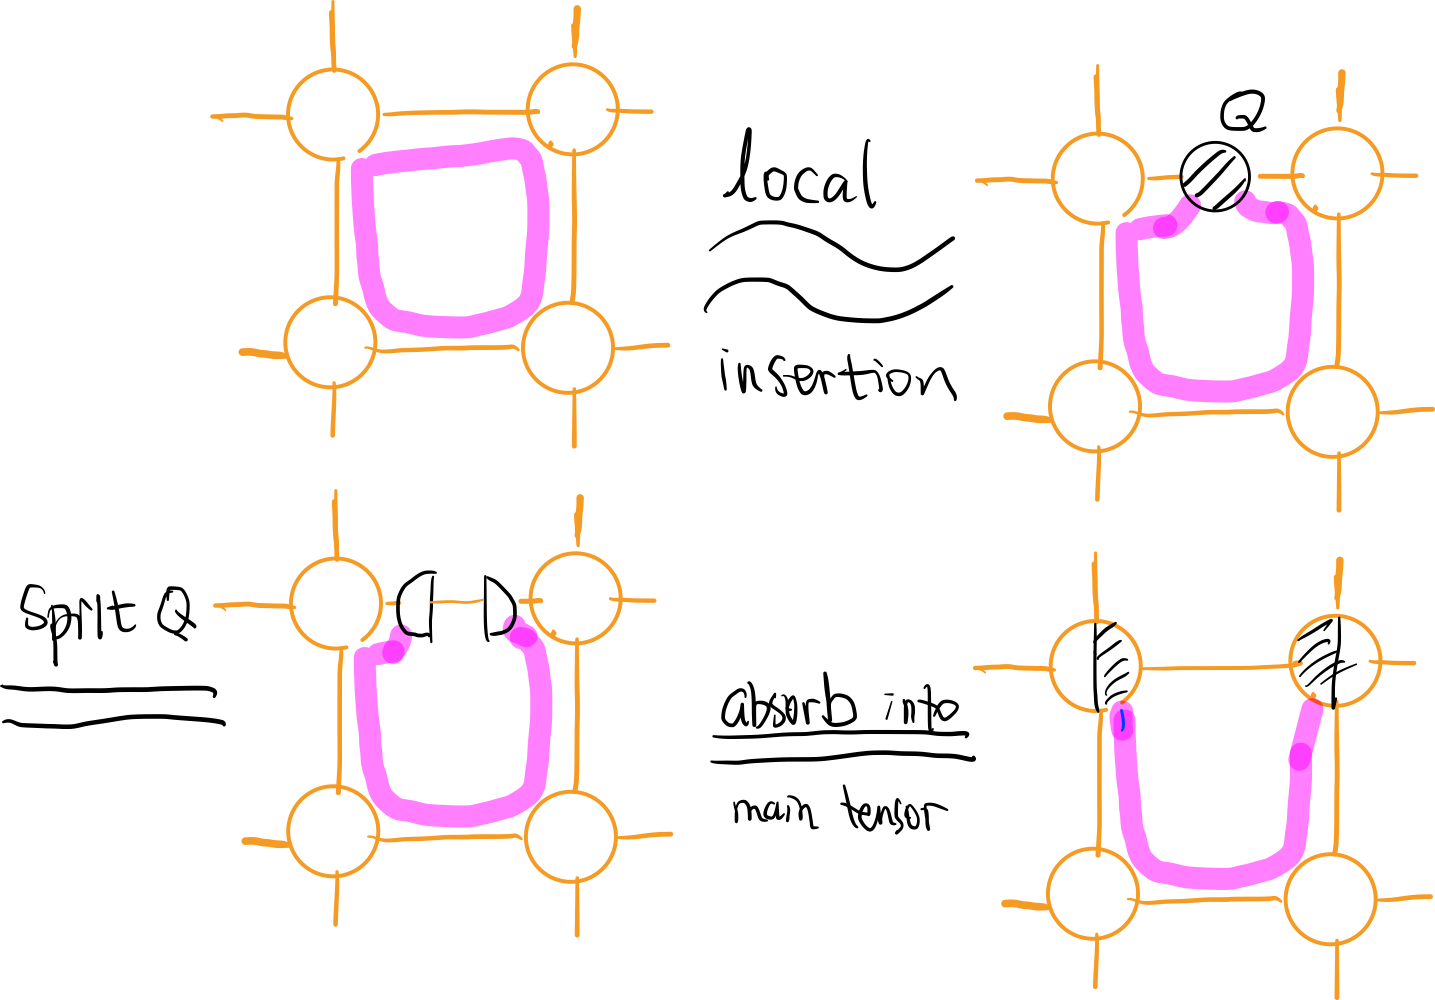
\includegraphics[width=7.5cm]{./figs/gilt}
    \caption{\label{fig:gilt}[\textbf{Add descriptions}]}
\end{figure}
%

However, since every insertion of a low-rank $Q$ matrix comes with an
approximation error, we should only perform the necessary truncations of
legs. We notice in Eq.~\eqref{eq:cdlHOTRG} that the HOTRG can take care
of four inner $C$ matrices, so it suffices for Gilt to filter out the
local interactions encoded in four outer $C$ matrices. In
Appendix~\ref{appd:cdlHOTRG}, we demonstrate how to choose the plaquette
and where to insert the $Q$ matrix. After Gilt filtering out all the
necessary legs, we perform the HOTRG coarse graining as usual. We call
this HOTRG armed with Gilt \textit{Gilt-HOTRG}. The coarse graining
process in the vertical direction goes similar as
Eq.~\eqref{def:Apycontr} except we apply halves of $Q$ matrices on $A$
tensors before applying the isometry $w$,
%
\begin{align}\label{def:ApycontrGilt}
    \begin{minipage}{2.0truecm}
      \centering
      
\includegraphics[width=1.8truecm,clip]{./figs/Ap-ycontr}
    \end{minipage}
    \defeq
    \begin{minipage}{4.0truecm}
      \centering
      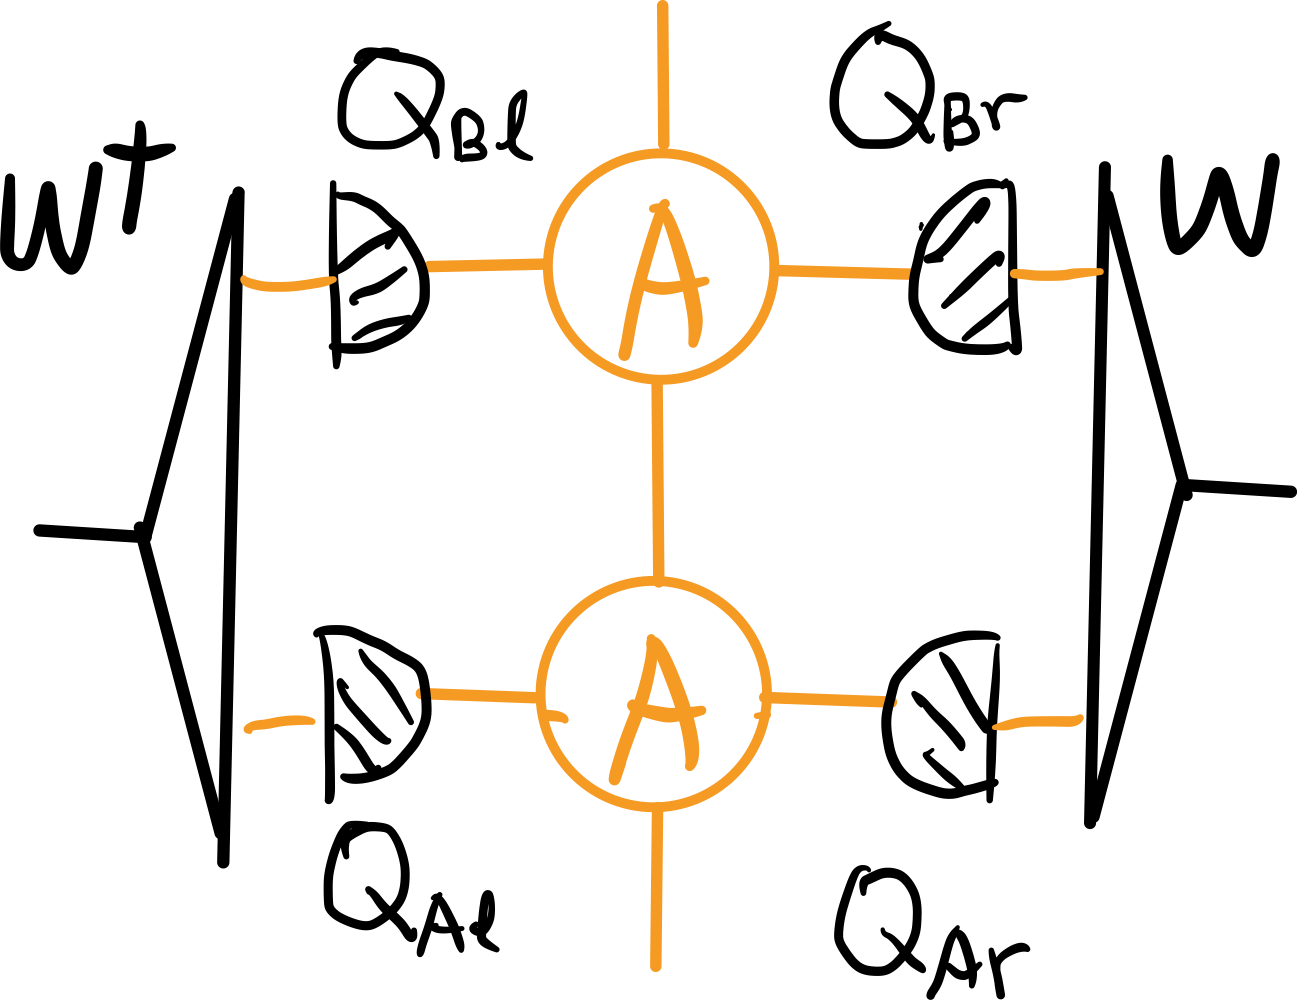
\includegraphics[width=3.8truecm,clip]{./figs/twoAgiltcoarse}
    \end{minipage},
\end{align}
%
where $Q_{Bl}$ and $Q_{Br}$ are two matrices obtained by splitting a
$Q_B$ matrix, $Q_B = Q_{Br}Q_{Bl}$, where $Q_B$ matirx is determined
using Gilt algorithm (see Appendix~\ref{appd:cdlHOTRG} for details).
$Q_{Al}$ and $Q_{Ar}$ are obtained in the same way. Then, we repeat the
similar Gilt truncations and HOTRG corse graining process in the
horizontal direction to have
%
\begin{align}\label{def:ApxcontrGilt}
    \begin{minipage}{2.0truecm}
      \centering
      
\includegraphics[width=1.8truecm,clip]{./figs/Ac-hotrg}
    \end{minipage}
    \defeq
    \begin{minipage}{4.0truecm}
      \centering
      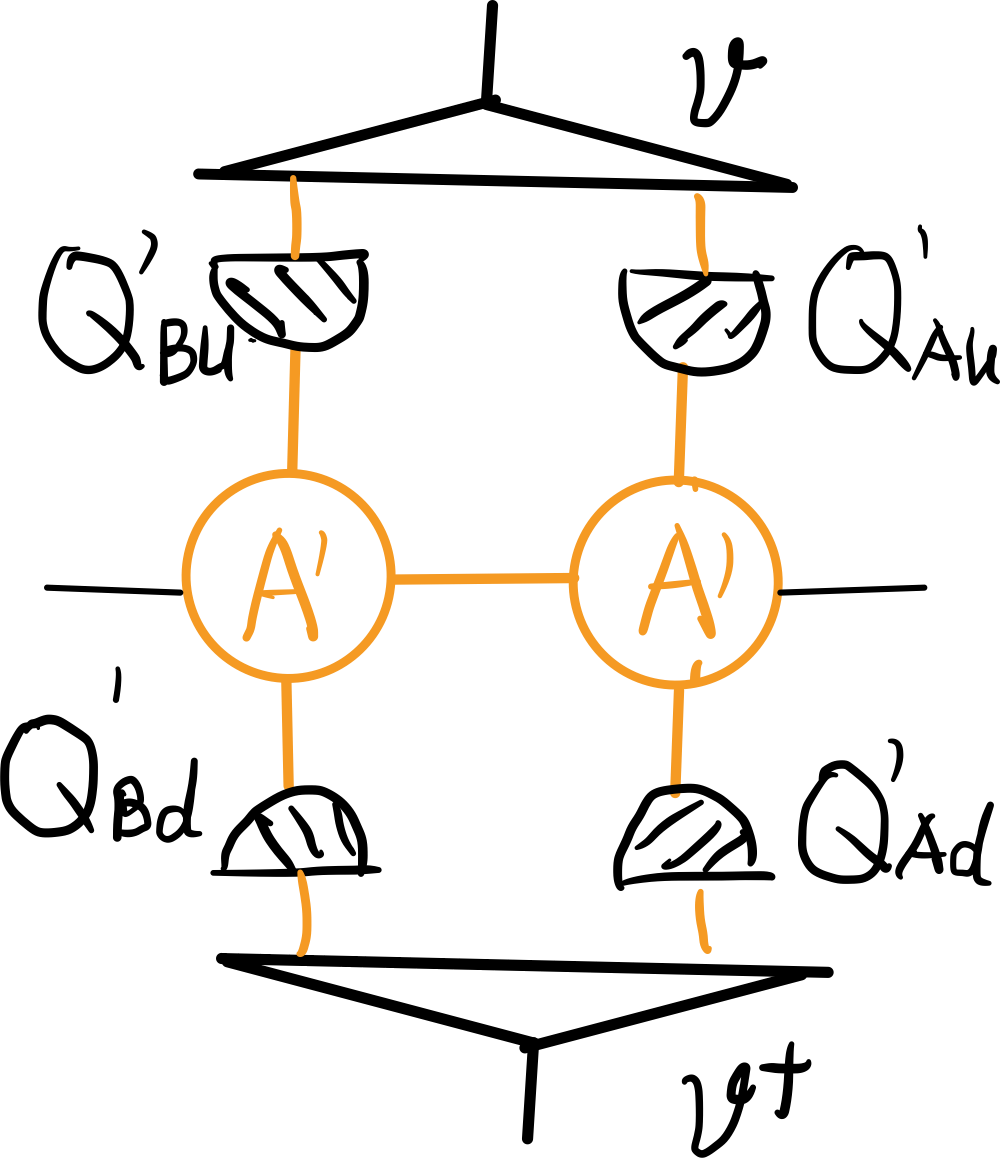
\includegraphics[width=3.8truecm,clip]{./figs/twoApgiltcoarse}
    \end{minipage}.
\end{align}
%
Equation~\eqref{def:ApycontrGilt} and~\eqref{def:ApxcontrGilt} together
defines the RG equation of Gilt-HOTRG
%
\begin{subequations}\label{def:RGeqGiltHOTRG}
    \begin{align}\label{def:RGeqGiltHOTRGschem}
    \begin{minipage}{2.0truecm}
        \centering
        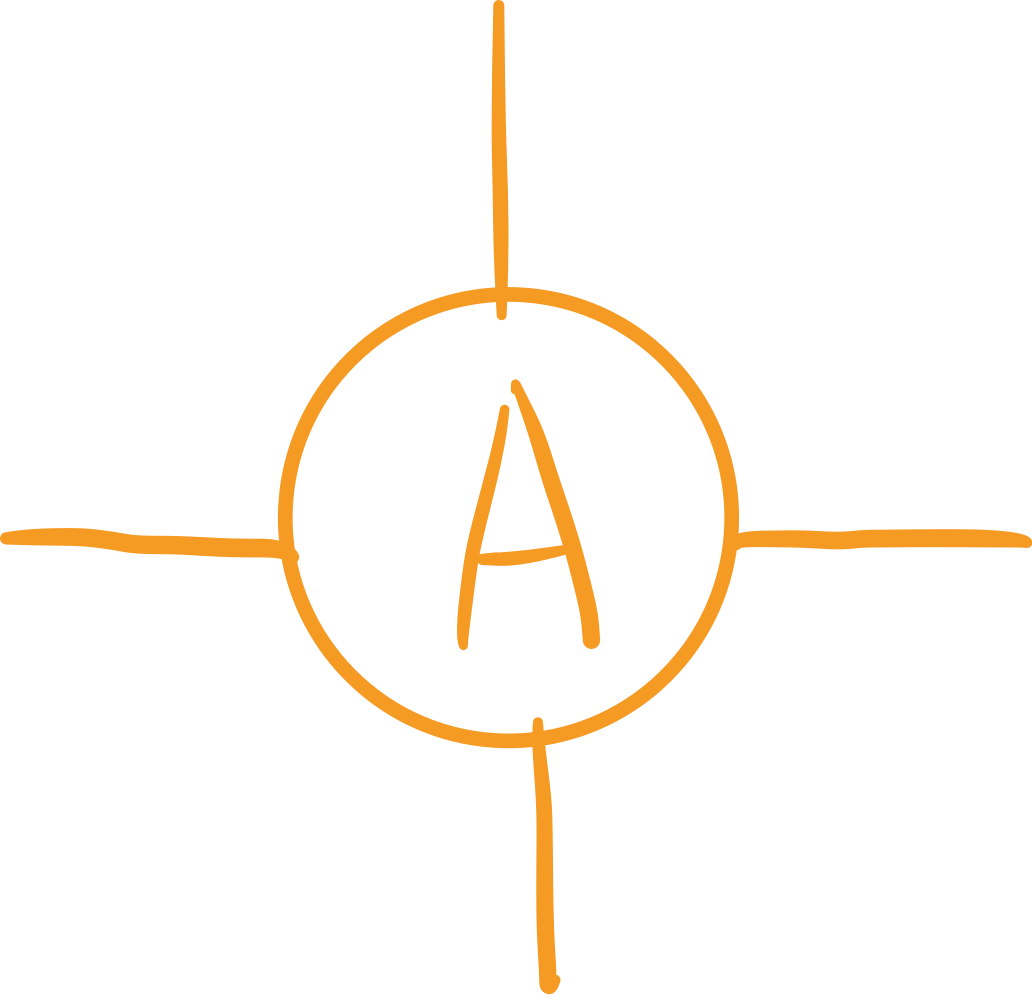
\includegraphics[width=1.8truecm,clip]{./figs/Aold}
    \end{minipage}
    &\xrightarrow{\text{Gilt-HOTRG}}
    \begin{minipage}{2.0truecm}
        \centering
        
\includegraphics[width=1.8truecm,clip]{./figs/Ac-hotrg}
    \end{minipage}
    \text{ or}\nonumber\\
    &A_c = \mathcal{T}\left(A\right). 
    \end{align}
or explicitly as
    \begin{align}\label{def:RGeqGiltHOTRGepl}
    \begin{minipage}{2.0truecm}
        \centering
        
\includegraphics[width=1.8truecm,clip]{./figs/Ac-hotrg}
    \end{minipage}
    = 
    \begin{minipage}{4.8truecm}
        \centering
        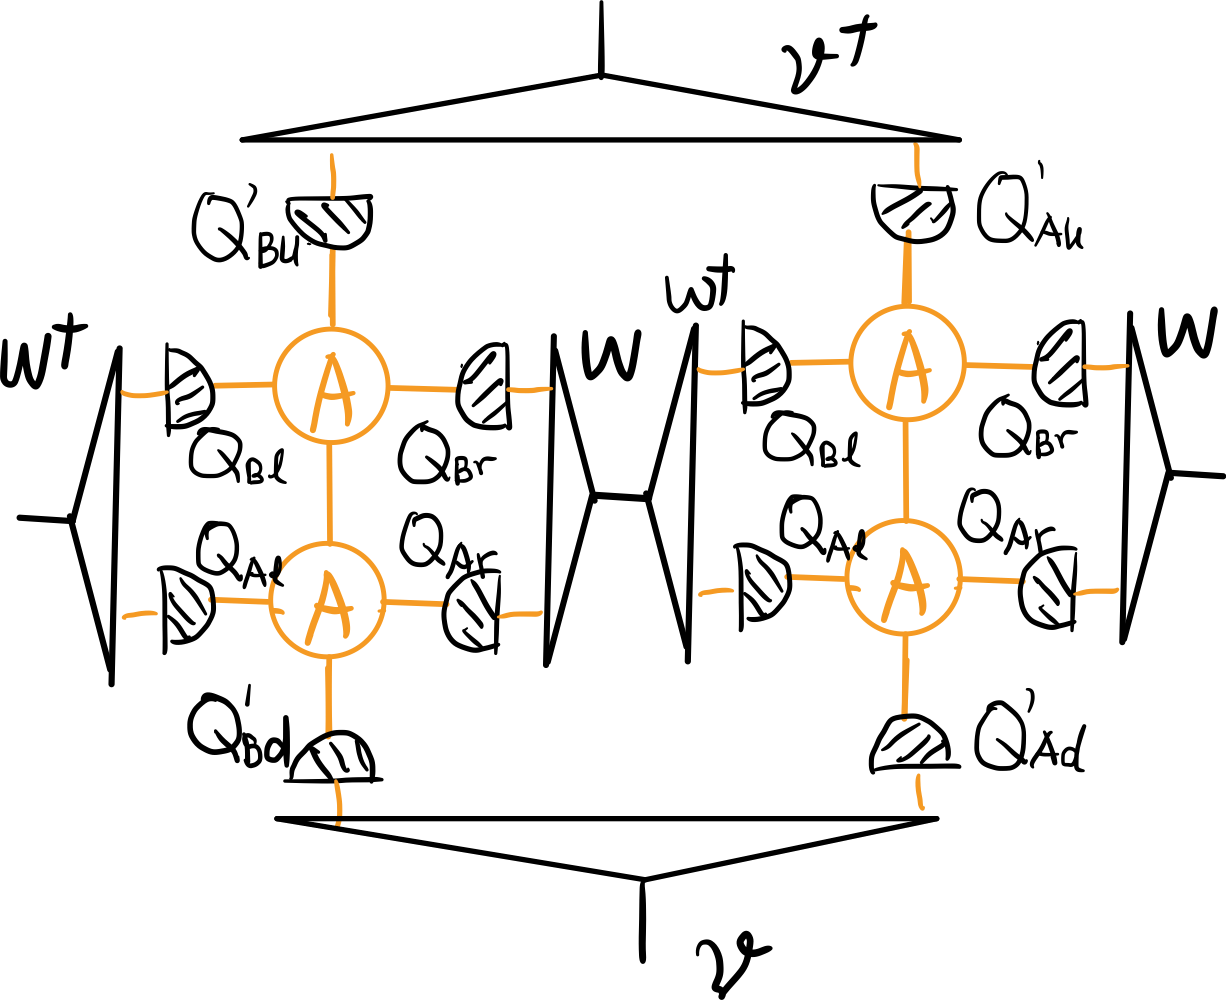
\includegraphics[width=4.6truecm,clip]{./figs/rgEq4GiltHOTRG}
    \end{minipage}.
    \end{align}
\end{subequations}
%
The coarse graining process defined in Eq.~\eqref{def:RGeqGiltHOTRG} is
able to simplify the $A^{\text{CDL}}$ tensor in Fig.~\ref{fig:ariseCDL}
to a single number (see Appendix~\ref{appd:cdlHOTRG} for detailed
calculations)
%
\begin{align}\label{eq:CDL2number}
    \begin{minipage}{2.0truecm}
        \centering
        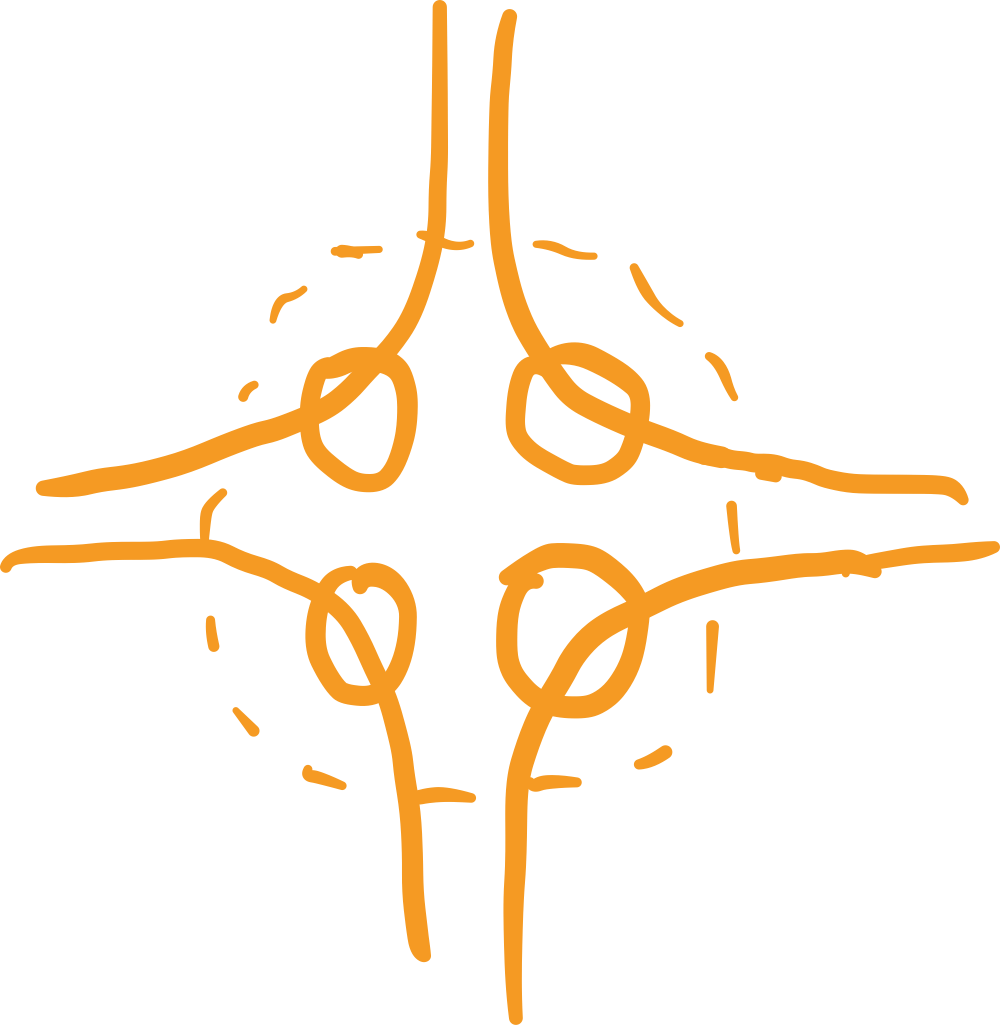
\includegraphics[width=1.8truecm,clip]{./figs/singleCDL}
    \end{minipage}
    \xrightarrow{\text{Gilt-HOTRG}}
    \left(\begin{minipage}{1.8truecm}
        \centering
        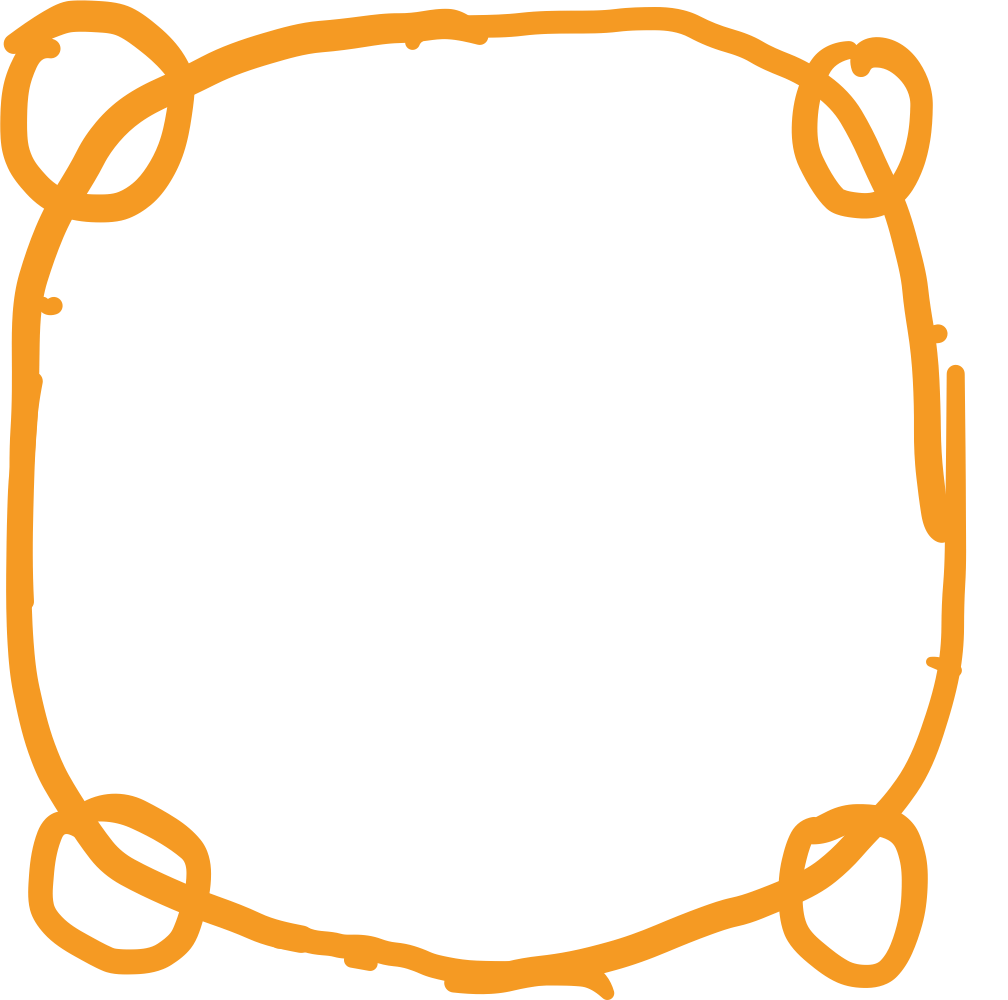
\includegraphics[width=1.6truecm,clip]{./figs/CDLnumber}
    \end{minipage}
    \right)^4.
\end{align}
%

Equation~\eqref{eq:CDL2number} shows that Gilt-HOTRG can sucessfully
filter out the local correlations among spin variables around the corner
at lattice scale (see Fig.~\ref{fig:ariseCDL}). Since CDL tensors are no
longer fixed points for the RG equation of Gilt-HOTRG, the pecular fixed
lines in Fig.~\ref{fig:tensorRGflow}(b) generated by HOTRG will collapse to
fixed points and we expect the RG equation of Gilt-HOTRG is able to
exhibit a critical fixed point tensor shown schematically in
Fig.~\ref{fig:tensorRGflow}(a).


\section{Response analysis\label{diffRGeq}}
Now we have the desired tensor block transformation, Gilt-HOTRG, which
can integrate out the local correlations and exhibit critical fixed
point tensors (we demonstrate this in Sec.~\ref{benchmark} by applying
Gilt-HOTRG to the 2D Ising model). The next step is to linearize the
tensor RG equation near a critical fixed point tensor and extract
scaling dimensions of the local operators in the CFT corresponding to
this fixed point. We will follow the convention in~\cite{kadanoff2014}
to call such an analysis \textit{response analysis}, and call the
linearized RG transformation in a certain representation
a \textit{response matrix}.
%

For people who are familiar with TRG-type tehcniques, the response
analysis might look straightforward. The response matrix is the
derivative of $A_c$ with respect to $A$ in
Eq.~\eqref{def:RGeqGiltHOTRGepl} evaluated at a fixed point tensor
$A^{*}$. The scaling dimensions $x_{\alpha}$ are related to the eigenvalues
$\lambda^{\alpha}$ of the response matrix through $b^{d-x_{\alpha}} =
\lambda^{\alpha}$, where $b$ is the RG rescaling factor and $d$ the
spatial dimension. For the RG equation of Gilt-HOTRG in
Eq.~\eqref{def:RGeqGiltHOTRGepl}, $b = 2$ and $d = 2$. 
%

However, there is a caveat to response analysis in tensor space: gauge
redundancy. To see how gauge redundancy arises in the new tensor
approach, it is informative to compare it with the conventional
approach. In this section, we will first give a review of response
analysis in the conventional RG approach. Then, we move on to tensor
response analysis and explain how it relates to the conventional
approach. The problem of gauge redundancy in tensor response analysis will
reveal itself during the comparision. Finally, we will introduce a
proper way to perform response analysis in tensor space using
Gilt-HOTRG.
%

\subsection{Response analysis in Hamiltonian space: a review of the old
approach}
It will be convenient to explain in terms of a specific physical system,
still a classical system spin variables $\sigma \in \{+1, -1\}$ on a
lattice, but with general short-ranged interactions (the short review
here follows this detailed review~\cite{kadanoff2014} and
textbook~\cite{cardy_1996} closely).  The Hamiltonian (or energy) of the
system can be described by a set of coupling constants $\mathbf{K} =
\{K_j\}$, each of which couples to a possible short-ranged interaction
term $s_j(\mathbf{r})$,
%
\begin{align}\label{eq:generalspinHam}
    \mathcal{H} = \sum_{\mathbf{r}} \sum_{j} K_j s_j(\mathbf{r}).
\end{align}
%
For example, if $K_1$ is the magnetic field, $s_1(\mathbf{r}) =
\sigma(\mathbf{r})$ is the spin variable at lattice point $\mathbf{r}$;
if $K_2$ is the nearest neighbor interaction along $x$ direction,
$s_2(\mathbf{r}) = \sigma(\mathbf{r})\sigma(\mathbf{r} +
a\hat{\mathbf{e}}_x)$, where $\hat{\mathbf{e}}_x$ is the unit vector
along $x$ direction and $a$ is the lattice constant. An RG transformation
will convert the old Hamiltonian $\mathcal{H}$ into a new Hamiltonian
$\mathcal{H}'$ \textit{with the same form as} Eq.~\eqref{eq:generalspinHam} but
characterized by a set of new coupling constants
$\mathbf{K}' = \{ K_j'\}$. The mapping from the old Hamiltonian to the
new Hamiltonian $\mathcal{H} \xrightarrow{\text{RG}} \mathcal{H}'$ is
then parametrized explicitly as the transformation from the old coupling
constants to the new coupling constants,
%
\begin{align}\label{eq:oldRGK}
    \mathbf{K}' = \mathcal{T}^{\text{old}}\left(\mathbf{K}\right).
\end{align}
%
We require that the RG transformation preserves the partition function of
the system and it must exhibit a fixed point Hamiltonian $\mathcal{H}^{*}$
described by coupling constants $\mathbf{K}^{*}$, such that they remain
unchanged under the RG transformation,
%
\begin{align}\label{eq:oldRGKstar}
    \mathbf{K}^{*} =
    \mathcal{T}^{\text{old}}\left(\mathbf{K}^{*}\right).
\end{align}
%
The response matrix is defined in the following way. We perturb the
coupling constants around the fixed point $\mathbf{K}_p = \mathbf{K}^{*}
+ \delta \mathbf{K}$ and perform an RG transformation defined in
Eq.~\eqref{eq:oldRGK}, $\mathbf{K}_p' = \mathcal{T}_{\text{old}}\left(
\mathbf{K}_p\right)$. The new coupling constants $\mathbf{K}_p'$ after
the RG transformation  should be close to $\mathbf{K}^{*}$ by
continuity, so $\mathbf{K}_p' = \mathbf{K}^{*} + \delta \mathbf{K}'$.
The response matrix $\mathcal{R}_{\text{old}}$ tells us how $\delta
\mathbf{K}'$ is related to $\delta \mathbf{K}$,
%
\begin{subequations}\label{eq:respMat}
    \begin{align}
    \delta \mathbf{K}' = \mathcal{R}^{\text{old}} \delta \mathbf{K},
    \end{align}
or in its component form,
    \begin{align}
        \delta K_i' = \sum_j\mathcal{R}^{\text{old}}_{ij} \delta K_j.
    \end{align}
\end{subequations}
%
Equation~\eqref{eq:respMat} is the definition of the response matrix,
which is nothing but the linearized RG equation around a fixed point
$\mathbf{K}^{*}$. The response matrix has right and left eigenvectors
$\{\psi^{\alpha}\}, \{\phi^{\alpha}\}$ with eigenvalues
$\{\lambda^{\alpha}\}$, so that
%
\begin{align}\label{eq:eigsofRespM}
    \sum_j \mathcal{R}^{old}_{ij} \psi^{\alpha}_j = \lambda^{\alpha}
    \psi^{\alpha}_i \text{ and } \sum_i \phi^{\alpha}_i
    \mathcal{R}^{old}_{ij} = \lambda^{\alpha} \phi^{\alpha}_j.
\end{align}
%
The linear combinations of $\delta K_i$ according to the components of the
left eigenvector $\phi^{\alpha}$ are known as scaling fields
%
\begin{align}\label{def:scalingfields}
    h^{\alpha} = \sum_i \phi^{\alpha}_i \delta K_i,
\end{align}
%
while the linear combinations of interaction terms $s_j(\mathbf{r})$
according to the componenets of the right eigenvector $\psi^{\alpha}$
are known as scaling operators
%
\begin{align}\label{def:scalingOpt}
    o^{\alpha}(\mathbf{r}) = \sum_j s_j(\mathbf{r}) \psi^{\alpha}_j.
\end{align}
%
Under an RG transformation with rescaling factor $b$ for a system in
dimension $d$, the scaling fields and the scaling operators transform in
a simpler way with $\left(h^{\alpha} \right)' = b^{d - x_{\alpha}}
h^{\alpha}$ and $\left(o^{\alpha}\right)' = b^{x_{\alpha}} o^{\alpha}$,
where $x^{\alpha}$ are the scaling dimensions of the scaling operators
$o^{\alpha}(\mathbf{r})$ and are related to the eigenvalues
$\lambda^{\alpha}$ of the response matrix through
%
\begin{align}\label{eq:lambda2x}
    b^{d-x_{\alpha}} = \lambda^{\alpha}.
\end{align}
%

In summary, in the conventional approach, we first find a fixed point
and determine the response matrix $\mathcal{R}^{\text{old}}$ at this
fixed point according to its definition in Eq.~\eqref{eq:respMat}. Then,
we find its eigenvalues $\lambda^{\alpha}$ and calculate scaling
dimensions according to Eq.~\eqref{eq:lambda2x}. Various critical
exponents can be calculated from these scaling dimensions if desired. 

\subsection{Response analysis in tensor space: gauge redundancy}
Na\"ively, repsonse analysis in tensor space can be carried out
in the same manner as the old approach. However, there is one more
complication in tensor approach: gauge redundancy.
%

In the conventional approach, we fix the form of the new Hamiltonian
$\mathcal{H}'$ to be the same as the old one $\mathcal{H}$ in
Eq.~\eqref{eq:generalspinHam}. They have the same interaction terms
$s_j(\mathbf{r})$ but coupled to different coupling constants
$\mathbf{K}$ and $\mathbf{K}'$. This gives a one-to-one correspondence
between a set of coupling constants $\mathbf{K} = \{K_j \}$ and a
Hamiltonian $\mathcal{H}$.

In a tensor block RG transformation $A \xrightarrow{\text{RG}} A_c$
defined in Eqs.~\eqref{eq:exactBlock} to~\eqref{eq:RGeqExact}, for
example, the only requirement is that the partition function should be
unchanged, and the new tensor $A_c$ could be express in a different set
of bases as the old tensor $A$. To be explicit, we say two tensors
$\tilde{A}$ and $A$ are \textit{equivalent} if they are related by the
following gauge transformation
%
\begin{subequations}\label{def:gaugeTrans}
    \begin{align}\label{def:gaugeTransMath}
        \tilde{A}_{ijkl} = \sum_{\substack{m,n\\p,q}} A_{mnpq} \left(S_x
        \right)_{im} \left(S_y \right)_{jn} \left(S_x^{-1}\right)_{pk}
        \left(S_y^{-1}\right)_{ql}, 
    \end{align}
or pictorially as
    \begin{align}\label{def:gaugeTransPic}
    \begin{minipage}{2.0truecm}
    \centering
    
\includegraphics[width=1.8truecm,clip]{./figs/Atilde}
    \end{minipage}
    =
    \begin{minipage}{3.0truecm}
      \centering
      
\includegraphics[width=2.8truecm,clip]{./figs/AsimilarTrans}
    \end{minipage},
    \end{align}
\end{subequations}
%
where $S_x, S_y$ are two invertible matices and $S_x^{-1},S_y^{-1}$
their inverses. If two tensors are similar, they describe the same
physics and it is easy to check that they will give the same partition
function. The gauge redundancy makes the correspondence between a tensor
$A$ and a physical system no long one-to-one. Instead, any element $A$
in its equivalence class defined in Eq.~\eqref{def:gaugeTrans} can be
selected to describe the physical system.
%

In fact, TRG-type techniques feature the exploiting of this gauge
redundancy in tensor network representations. For HOTRG described in
Sec.~\ref{hotrg}, we use eigenvectors defined in
Eq.~\eqref{eq:optwCondi} as good bases since their importance is
reflected by the corresponding eigenvalues. Several unimportant bases
are thrown away and a change of horizontal bases of a patch of two $A$
tensors is performed in Eq.~\eqref{def:Apycontr} using an isometry
$w^{\dagger}$ as $S_x$ to define the coarse graining in the vertical
direction.
%

However, gauge redundancy makes response analysis in tensor space less
straighforward than the old approach. Even when we have reached a fixed
point, the RG transformation in tensor space could bring one element in
an equivalence class to another one in the same equivalence class, $A^*
\xrightarrow{\text{RG}} \tilde{A}^*$. In general, we must fix the gauge
of the tensor during an RG transformation by choosing a prefered set of
bases, so that the fixed point tensor is manifestly fixed under the RG
transformation, $A^* \xrightarrow{\text{RG}} A^*$, or written in a
similar fashion to Eq.~\eqref{eq:oldRGKstar},
%
\begin{align}\label{eq:tensorRGAstar}
    A^* = \mathcal{T}^{\text{ten}}\left(A^* \right).
\end{align}
%
We will show how the gauge is fixed in Gilt-HOTRG to achieve
Eq.~\eqref{eq:tensorRGAstar} in Sec.~\ref{RespAnaGiltHOTRG}.
%

After gauge fixing is done, the rest is exactly the same as the old
approach. We linearize the tensor RG transformation near the fixed point
tensor $A^*$ by adding a perturbation $\delta A$ and studying how it
transforms to $\delta A_c$ after corase graining. This gives the
response matrix in tensor space,
%
\begin{align}\label{eq:respMatTen}
    \left(\delta A_c\right)_{(i)} = \sum_j
    \mathcal{R}^{\text{ten}}_{(i)(j)} \delta A_{(j)},
\end{align}
%
where we have grouped the four legs of the tensor into a single leg,
$\delta A_{(j)} \defeq \delta A_{j_1 j_2 j_3 j_4}$. The eigenvalues of
the response matrix $\mathcal{R}^{\text{ten}}$ then give the sclaing
dimensions of the scaling operators in the CFT corresponding to this
fixed point according to Eq.~\eqref{eq:lambda2x}.
%

In the discussions above, we show, by analogy to the old approach, how
to perform response analysis in tensor space. There is one last thing
that needs to be clarified. We assume that the tensor $A$, after proper
gauge fixing, plays the same role as the coupling constants
$\mathbf{K}$ does in the old approach. We provide the justification of
this assumption in the next subsection.
%


\subsection{Relation between response analysis in tensor space and that
in Hamiltonian space\label{relateTensorCoupling}}
In the old approach, the RG flow of Hamiltonians is parameterized by a
flow in coupling constants space $\mathbf{K}$ after various interaction
terms $s_j(\mathbf{r})$ are given. In the tensor approach, we skip the
Hamiltonian description of the system. Insteand, we use a tensor $A$
that encodes Boltzamann weight of local configurations to describe the
system. The RG flow is then parameterized by a flow in tensor space. We
claim that the components of the tensor $A$ can be thought of as some
proxies of the coupling constants $\mathbf{K}$.
%

To see why this claim is reasonable, note that we can map the partition
function of the system with Hamiltonian~\eqref{eq:generalspinHam} into a
tensor network using the method introduce in Sec.~\ref{spin2tensor} and
in Ref.~\cite{trg}. Each component of the initial tensor $A$ is the
Boltzmann weight of a given local configuration that depends on the
coupling constants, so we have 
%
\begin{align}\label{eq:K2A}
    A_{(i)} = f_{(i)}\left(\mathbf{K}\right),
\end{align}
%
where we group all legs of $A$ to form a single index. After coarse
graining, the componenets of $A_c$ are still functions of $\mathbf{K}$ but
with different functional forms,
%
\begin{align}\label{eq:tensorEleRG}
    \left(A_c\right)_{(i)} =
\left(f_c\right)_{(i)}\left(\mathbf{K}\right).
\end{align}
%
Now, imagine we have imposed the gauge fixing condition by requiring the
same functional form as old tensor $A$ but with different coupling
constants $\mathbf{K}'$, 
%
\begin{align}\label{eq:tensorK2Kp}
    f_{(i)}\left(\mathbf{K}'\right) =
    \left(f_c\right)_{(i)}\left(\mathbf{K}\right), \forall (i).
\end{align}
%
In the old approach, we need to solve Eq.~\eqref{eq:tensorK2Kp} for
$\mathbf{K}'$ in terms of $\mathbf{K}$, which defines the RG equation
from the old $\mathbf{K}$ to the new $\mathbf{K}'$. However, in the
tensor approach, it is enough to know the existence of such
$\mathbf{K}'$. Combine Eq.~\eqref{eq:tensorEleRG} and
Eq.~\eqref{eq:tensorK2Kp}, we have
%
\begin{align}\label{eq:Kp2A}
    \left(A_c\right)_{(i)} = f_{(i)}\left(\mathbf{K}'\right).
\end{align}
%
Take the total derivative of tensor $A$ and $A_c$ in Eqs.~\eqref{eq:K2A}
and \eqref{eq:Kp2A} and set $\mathbf{K} = \mathbf{K}' = \mathbf{K}^*$,
%
\begin{align}
    \delta A_{(i)} = \sum_n \left(\partial_{(n)}
    f_{(i)}\right)\Bigr|_{\mathbf{K} = \mathbf{K}^*} \delta K_n,
    \label{eq:deltaK2deltaA} \\
    \left(\delta A_c \right)_{(i)} = \sum_n \left(\partial_{(n)}
    f_{(i)}\right)\Bigr|_{\mathbf{K}' = \mathbf{K}^*} \delta
    K_n'.\label{eq:deltaK2deltaAp}  
\end{align}
%
Equations~\eqref{eq:deltaK2deltaA} and \eqref{eq:deltaK2deltaAp} explain
the relation between response analysis in tensor space defined in
Eq.~\eqref{eq:respMatTen} and that in Hamiltonian space defined in
Eq.~\eqref{eq:respMat}. They are the same linear transformation in two
different representations, with $\partial_{(n)}f_{(i)}$ evaluated at
$\mathbf{K}^*$ being the change of basis matrix.
%

In Sec.~\ref{benchmark:1DIsing}, we will use 1D Ising model as a
concrete example to demonstrate the general argument above.
%

\subsection{Response analysis of Gilt-HOTRG\label{RespAnaGiltHOTRG}}
We will introduce a way to fix the gauge redundancy and give the
explicit expression of the response matrix for Gilt-HOTRG in this
subsection.
%

Part of the gauge redundancy can be fixed if the physical model
possesses a global internal symmetry. The global symmetry can be
incorporate into the tensor network representation of the
model~\cite{Singh2010SymTen,Singh2011U1Ten,Singh2012SU2Ten}, which is a
generalization of Schur's lemma applicable for general symmetric
tensors. For example, classical Ising model with only the
nearest-neighbor interaction has $\mathbb{Z}_2$ symmetry. In its tensor
network representation, each leg of the tensor $A$ will break into even
and odd sectors. Half of the gauge redundancy will be fixed by going to
the bases where the states in the even sector transform trivially and
the states in the odd sector is multiplied by $-1$ under spin flip
transformation.
%

Most part of the remaining gauge redundancy can be automatically fixed
during Gilt-HOTRG due to the following property of Gilt-HOTRG, whose
proof will be provided in Appendix~\ref{appd:gaugeFix}. For two tensors
$A, \tilde{A}$ that are related by the gauge transformation defined in
Eq.~\eqref{def:gaugeTrans} where we further restrict $S_x,S_y$ to be
orthogonal matrices (or unitray matrices if $A, \tilde{A}$ are complex),
the new tensors produced by Gilt-HOTRG coarse graining according to
Eq.~\eqref{def:RGeqGiltHOTRG}, $A_c = \mathcal{T}\left(A\right),
\tilde{A}_c = \mathcal{T}(\tilde{A})$ are equal up to sign ambiguities.
The sign ambiguities can be easily fixed by comparing components of
$A_c$ and $\tilde{A}_c$. After adding a sign fixing step in Gilt-HOTRG,
we will have
%
\begin{align}\label{eq:HOTRGgaugefix}
    \mathcal{T}(A) = \mathcal{T}(\tilde{A}).
\end{align}
%
Since the orthgonal matrices $S_x, S_y$ are arbitrary,
Eq.~\eqref{eq:HOTRGgaugefix} says that the whole equivalence class tensor
$A$ lives in will be mapped into the same tensor $A_c$. This means
that Gilt-HOTRG, after incorporating the sign fixing step, will choose a
preferred set of bases. It is worth to mention that TRG has this
property too~\cite{kadanoff2014}.
%

For a fixed-point tensor, Eq.~\eqref{eq:HOTRGgaugefix} indicates that we
can start with any element $\tilde{A}^*$ in the equivalence class, and
Gilt-HOTRG will bring this tensor to the proper bases where further
Gilt-HOTRG coarse graining will give a manifestly fixed-point tensor
%
\begin{align}\label{eq:GiltHOTRGfixT}
    \mathcal{T}(\tilde{A}^*) =
    \mathcal{T}\left(\mathcal{T}(\tilde{A}^*)  \right) = A^*.
\end{align}
%
This leaves us a question of why we can restrict invertible matices
$S_x, S_y$ to be orthogonal. [\textbf{Should we explain it here, or
define the gauge transformation using orthogonal matrices directly?}]
% TODO
%

After reaching the fixed-point tensor $A^*$, we should linearize the RG
equation of Gilt-HOTRG in Eq.~\eqref{def:RGeqGiltHOTRG} to obtain the
response matrix $\mathcal{R}$. We substitute $A = A^* + \delta A$ into
the right hand side of Eq.~\eqref{def:RGeqGiltHOTRGepl} and collect
terms that are first order in $\delta A$ to get $\delta A_c$,
%
\begin{widetext}
    \begin{align}\label{eq:respMatGiltHOTRG}
    \begin{minipage}{2.0truecm}
    \centering
    
\includegraphics[width=1.8truecm,clip]{./figs/deltaAc}
    \end{minipage}
    &=
    \begin{minipage}{5.0truecm}
    \centering
    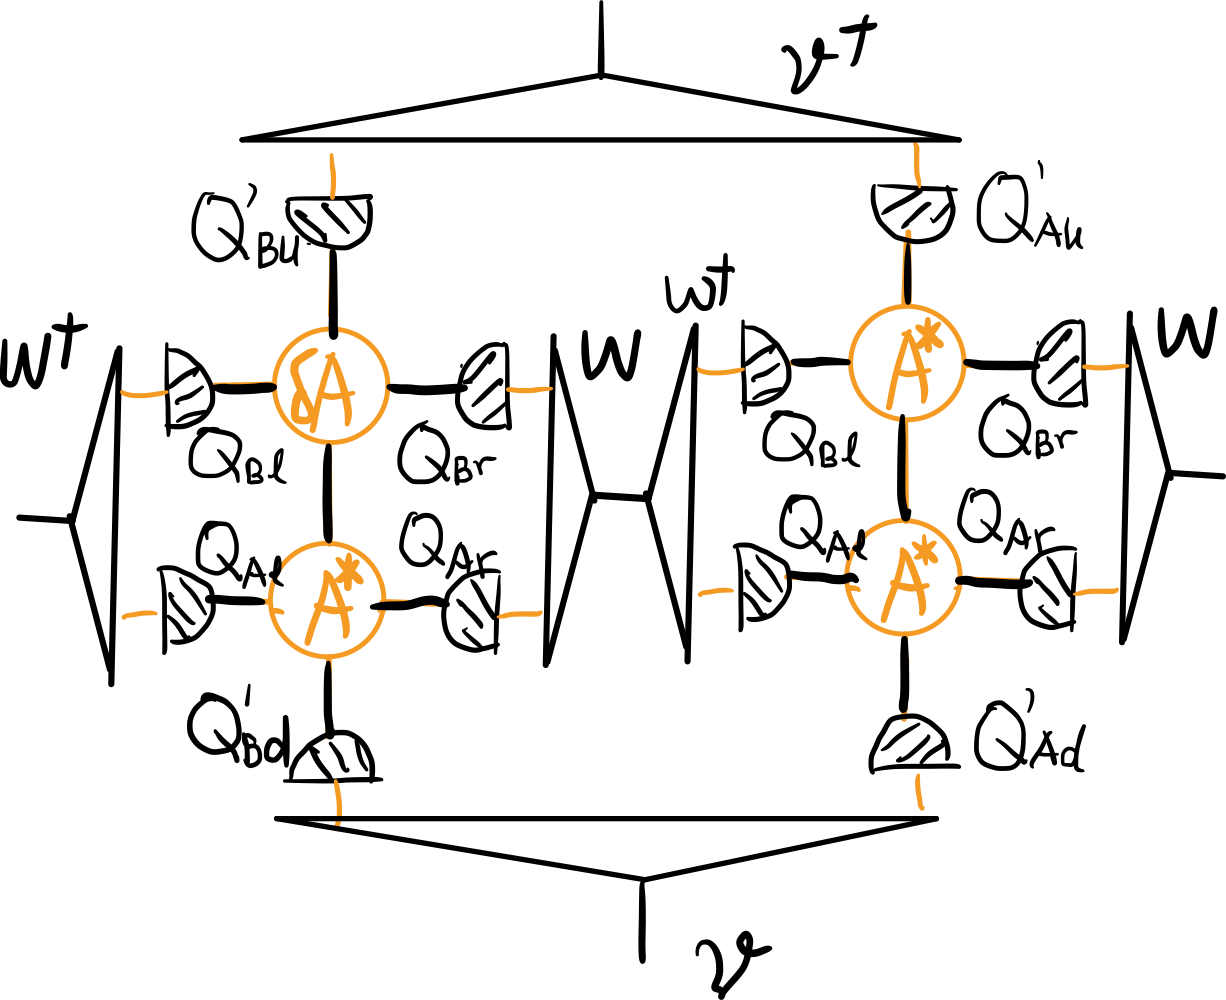
\includegraphics[width=4.8truecm,clip]{./figs/deltaA1}
    \end{minipage}
    +
    \begin{minipage}{5.0truecm}
    \centering
    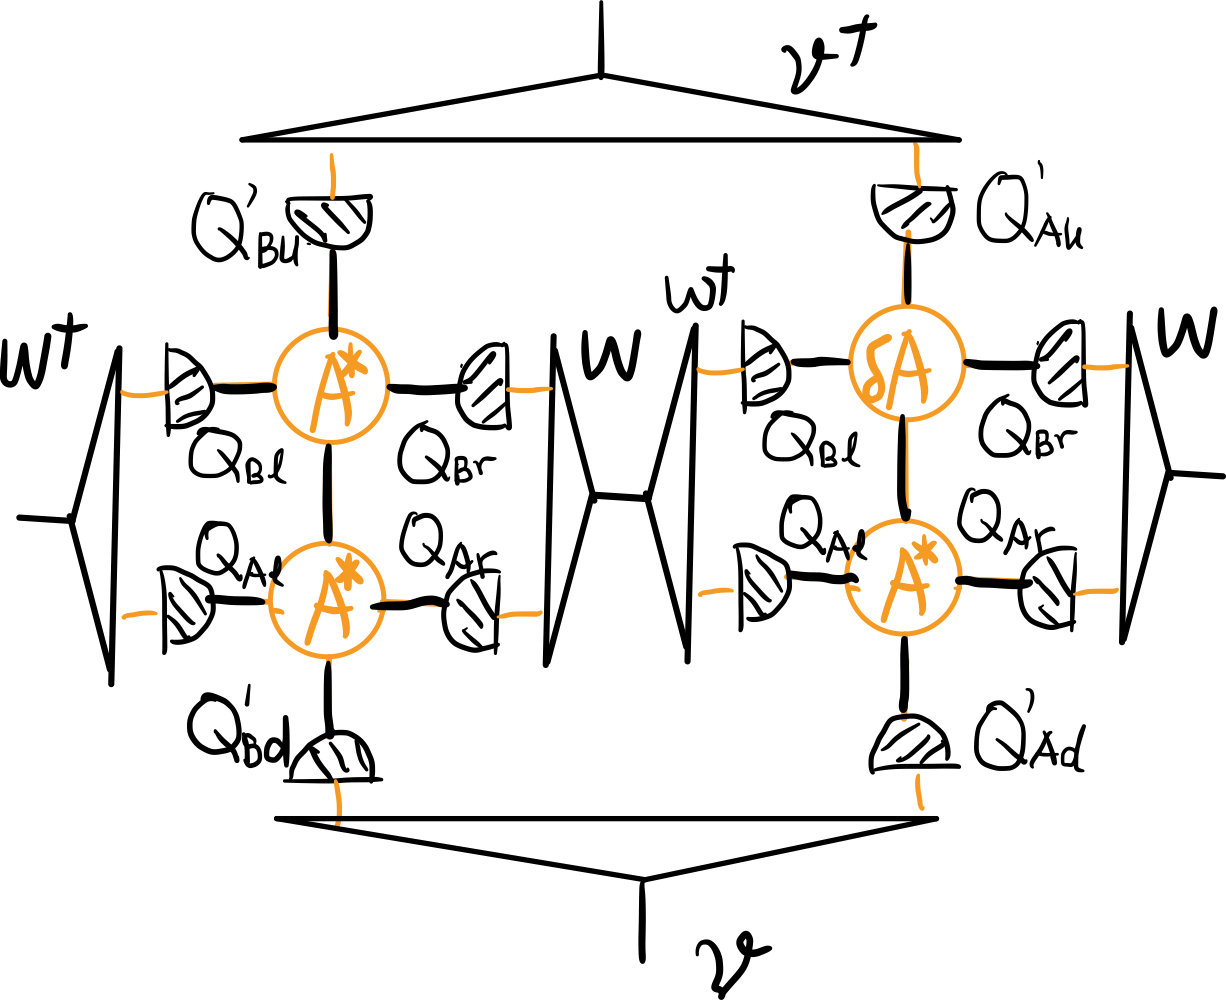
\includegraphics[width=4.8truecm,clip]{./figs/deltaA2}
    \end{minipage} %\nonumber\\
%    &+
%    \begin{minipage}{5.0truecm}
%    \centering
%    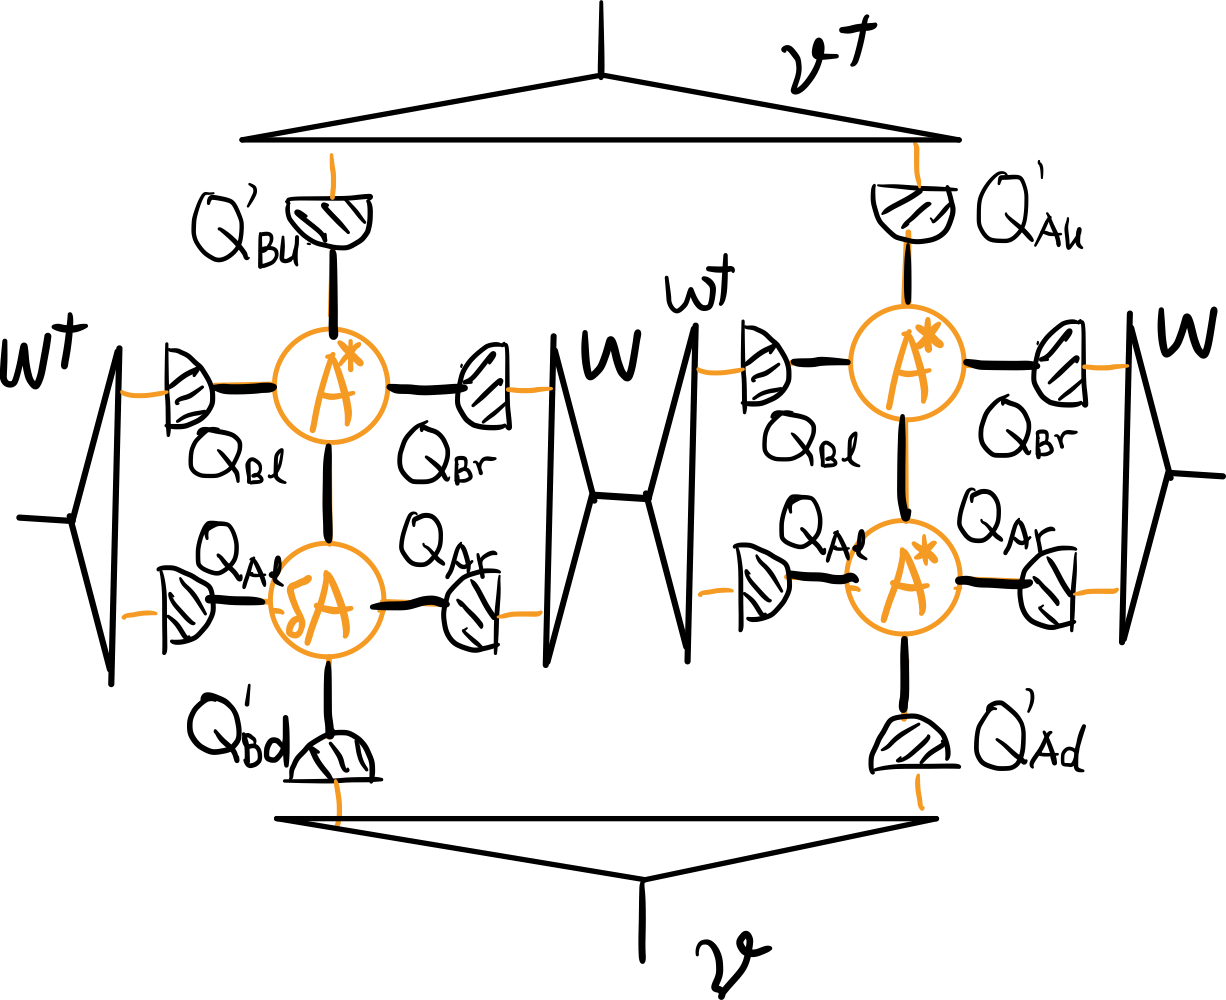
\includegraphics[width=4.8truecm,clip]{./figs/deltaA3}
%    \end{minipage}
%    +
%    \begin{minipage}{5.0truecm}
%    \centering
%    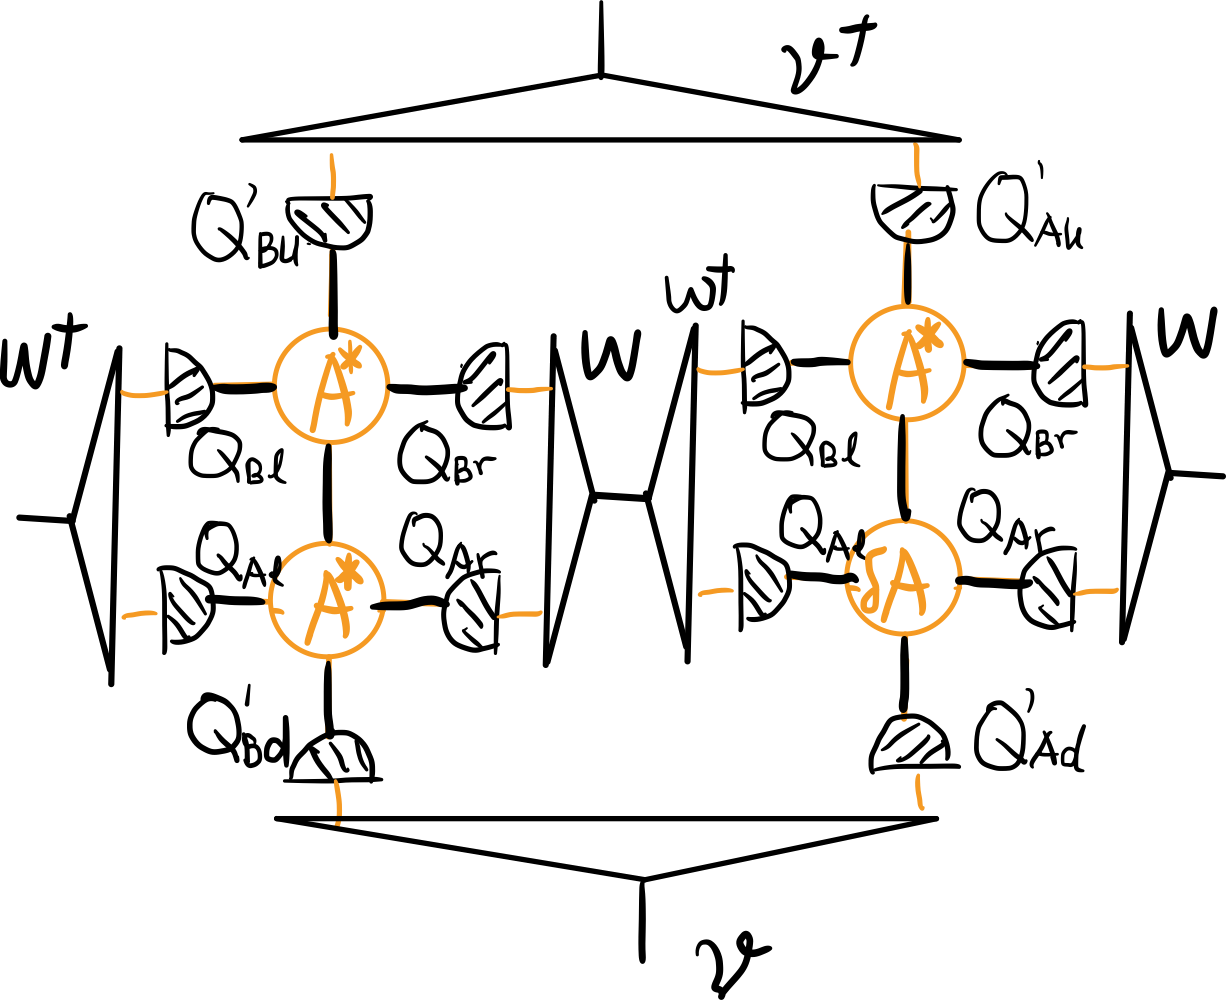
\includegraphics[width=4.8truecm,clip]{./figs/deltaA4}
%    \end{minipage}
    + \text{ two more terms}.
    \end{align}
\end{widetext}
%
The result resembles the product rule for taking the differentials in
calculus. Equation~\eqref{eq:respMatGiltHOTRG} provides a nice pictorial
representation of how the response matrix $\mathcal{R}$ for Gilt-HOTRG
acts on the perturbation $\delta A$ around a fixed-point tensor $A^*$.
In practice, after the fixed-point tensor $A^*$, low-rank matrices $Q$
's and isometric tensors $w, v$ in Eq.~\eqref{def:RGeqGiltHOTRGepl} are
determined, automatic differentiation techniques can linearize
Eq.~\eqref{def:RGeqGiltHOTRGepl} around $A^*$ and generate the action of
response matrix described in Eq.~\eqref{eq:respMatGiltHOTRG} for us.
There are many libraries that support automatic differntiation,
including PyTorch~\cite{pytorch} and JAX~\cite{jax2018github}.
%

% TODO
[\textbf{Add justifications for why we can ignore corrections coming from
isometric tensors and low-rank matrices.}]

\section{Benchmark results\label{benchmark}}
We use 1D and 2D classical Ising models to demonstrate how to carry out
a reponse analysis in tensor space. Ising model in 1D serves as a
concrete example to elucidate the connection with the old approach, the
general argument of which is in Sec.~\ref{relateTensorCoupling}. Ising
model in 2D provides more nontrivial benchmark results for our method.
%

\subsection{Ising Model in 1D\label{benchmark:1DIsing}}
Ising model in 1D has an exact real-space RG transformation realized via
decimation. Even better, the decimation process has a natural tensor
network represention. This makes Ising model in 1D a nice example to see
the relation between the old and the new approaches of response
analysis.
%

The partition function is
%
\begin{align}\label{def:Z4Ising1D}
    Z_{\text{1D}} = \sum_{\{\sigma_j \} } \exp{\left[\sum_{i=1}^N
    \mathscr{H}\left(\sigma_i,\sigma_{i+1}\right)  \right]},
\end{align}
%
where the local interactions involve nearest-neighbor at most
%
\begin{align}\label{def:H4Ising1D}
    \mathscr{H}\left(\sigma_1, \sigma_2\right) = g +
    \frac{h}{2}\left(\sigma_1 + \sigma_2\right) + K\sigma_1 \sigma_2.
\end{align}
%
The decimation process is shown in Fig.~\ref{fig:Ising1D-decimation},
and it is realized by summing over all the even numbered spins and then
renumber the remaining odd numbered spins. 
%
\begin{figure}[h]
    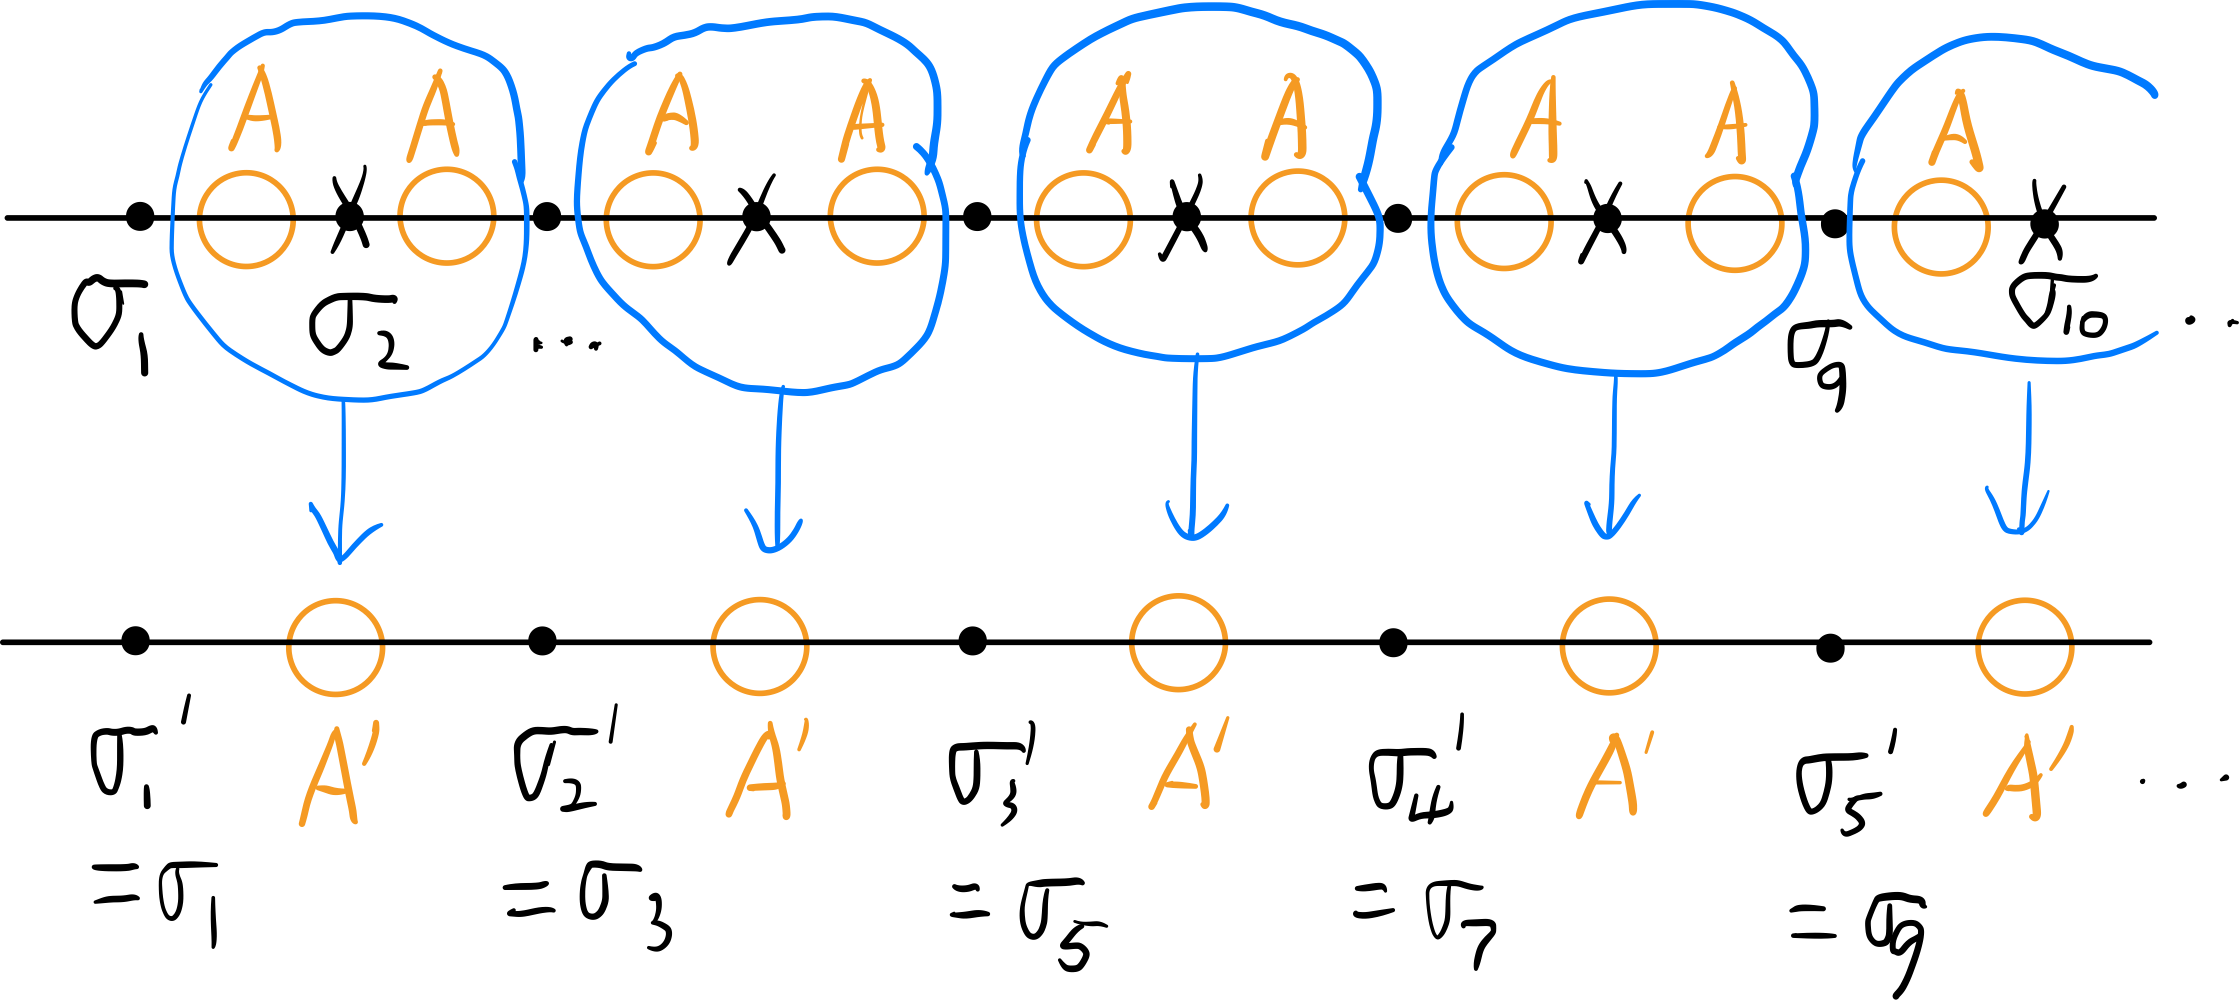
\includegraphics[width=7.5cm]{./figs/Ising1D-decimation}
    \caption{\label{fig:Ising1D-decimation}[\textbf{Add descriptions}]}
\end{figure}
%

We denote $\sigma_i'=\sigma_{2i-1}, s_i = \sigma_{2i}$ and sum over all
$s$-spins in the partition function in Eq.~\eqref{def:Z4Ising1D} to have
%
\begin{align}\label{eq:oldK2newKZ}
    Z_{\text{1D}} = \sum_{\{\sigma_j'\}} \sum_{\{s_j \}}
    \exp{\left[ \sum_i^{N/2} \left[\mathscr{H}\left(\sigma_i',s_i\right)
    + \mathscr{H}\left(s_i,\sigma_{i+1}'\right)\right]\right]},
\end{align}
%
from which we can define the effective local interaction $\mathscr{H}'$
through
%
\begin{align}\label{eq:oldK2newK}
    \exp{\left[\mathscr{H}'\left(\sigma_1',\sigma_2'\right)\right]} =
    \sum_{s=\pm 1}\exp{\left[\mathscr{H}\left(\sigma_1',s\right) +
        \mathscr{H}\left(s,\sigma_2'\right)\right]},
\end{align}
%
where the effective local interaction has the same form as the old one
in Eq.~\eqref{def:H4Ising1D} but with new coupling constants $g',h',K'$,
%
\begin{align}\label{def:newH4Ising1D}
    \exp{\left[\mathscr{H}'\left(\sigma_1,\sigma_2\right)\right]} = g' +
    \frac{h'}{2}\left(\sigma_1 + \sigma_2\right) + K' \sigma_1 \sigma_2.
\end{align}
%
The partition function can be fully described by new $\sigma'$-spins,
%
\begin{align}\label{eq:Z2Ising1Dnew}
    Z_{\text{1D}} = \sum_{\{\sigma_j'\}}
    \exp{\left[\sum_{i=1}^{N/2}\mathscr{H}'\left(\sigma_i',\sigma_{i+1}'\right)\right]}.
\end{align}
%
Equations~\eqref{def:H4Ising1D}, \eqref{eq:oldK2newKZ}
and~\eqref{def:newH4Ising1D} together define the RG equation that maps
the old coupling constatns $(g,h,K)$ into the new coupling constants
$(g',h',K')$. The explicit expression of the RG equation can be found in
Kardar's textbook~\cite{kardar2007}. The RG equation has two fixed
points, one for high temperature phase and the other for low temperature
phase. Let us focus on the high temperature fixed point here, where the
coupling constants are $g^* = \log\left(1/2\right),h^*=0,K^*=0$. The
linearized RG equation around this fixed point gives $\delta g' =
2\delta g, \delta h' = \delta h, \delta K' = 0\times \delta K$. The
response matrix is in its diagonal form with eigenvalues $2,1,0$ for
$\delta g,\delta h,\delta K$ repectively.
%

Next, we translate the above decimation process into tensor network
language. We first define the tensor $A$ sitting on the bound connecting two
spins shown in Fig.~\ref{fig:Ising1D-decimation} as
%
\begin{subequations}\label{def:A4Ising1D}
    \begin{align}\label{def:A4Ising1DCompo}
    A_{\sigma_1 \sigma_2} =
    \exp{\left[\mathscr{H}\left(\sigma_1,\sigma_2\right)\right]},
    \end{align}
    after using the expression for $\mathscr{H}$ in
    Eq.~\eqref{def:H4Ising1D}, we have
    \begin{align}\label{def:A4Ising1Depl}
        A = 
    \begin{pmatrix}
    \exp{\left(g + h + K\right)} & \exp{\left(g - K\right)} \\
    \exp{\left(g - K\right)} & \exp{\left(g - h + K\right)} \\
    \end{pmatrix},
    \end{align}
\end{subequations}
%
which is the familiar transfer matrix. Each component of the tensor $A$ is
a function of coupling constants $g, h, K$, as is claimed in
Eq.~\eqref{eq:K2A}. The partition function in Eq.~\eqref{def:Z4Ising1D}
can be rewritten as
%
\begin{align}\label{eq:Z4Ising1DbyA}
    Z_{\text{1D}} = \sum_{\{\sigma_j\}} \prod_{i=1}^N A_{\sigma_i
        \sigma_{i+1}}.
\end{align}
%
The decimation process in tensor network language is multplication of
two old $A$ matrices to form a new $A_c$ matrix,
%
\begin{align}\label{def:Ising1DRGeqTen}
    A_c = AA.
\end{align}
%
In terms of the new $A'$ matrix, the partition function is
%
\begin{align}\label{eq:Z4Ising1DbyAp}
    Z_{\text{1D}} = \sum_{\{\sigma_j'\}} \prod_{i=1}^{N/2}
    (A_c)_{\sigma_i' \sigma_{i+1}'}.
\end{align}
%
Equation~\eqref{def:Ising1DRGeqTen} is the RG equation in tensor network
language. Now, each component of $A_c$ is a function of coupling
constants $g,h,K$ but with different functional form, as is claimed in
Eq.~\eqref{eq:tensorEleRG}. If we further require $A_c$ has the same
form as $A$ in Eq.~\eqref{def:A4Ising1D} but with $\mathscr{H}$ replaced
by $\mathscr{H}'$, new coulping constants $g',h',K'$ can be solved in
terms of old ones, which is what we do in the conventional approach. The
advantange of using tensor network language is that RG equation in
Eq.~\eqref{def:Ising1DRGeqTen} suffices for the response analysis in
tensor space. First, let us set coupling constants in
Eq.~\eqref{def:A4Ising1Depl} to be the high temperature fixed point
$g^* = \log{\left(1/2\right)}, h^*=0, K^* = 0$ to get the fixed-point
tensor,
%
\begin{align}\label{eq:fixedA4Ising1D}
    A^* = \frac{1}{2}
\begin{pmatrix}
    1 & 1 \\
    1 & 1 \\
\end{pmatrix}.
\end{align}
%
It can be checked that $A^* A^* = A^*$. The linearized version of
Eq.~\eqref{def:Ising1DRGeqTen} around this fixed-point tensor is
%
\begin{align}\label{eq:Ising1DRespEq}
    \delta A_c = \delta A A^* + A^* \delta A = I \delta A A^* + A^*
    \delta A I,
\end{align}
%
where in the last equal sign, we add two identity matrices. Write
Eq.~\eqref{eq:Ising1DRespEq} in its component form, we have
$\left(\delta A_c\right)_{ab} =
\sum_{\alpha,\beta}I_{a\alpha}\left(\delta A\right)_{\alpha\beta}
\left(A^*\right)_{\beta b} + \left(A^*\right)_{a\alpha} \left(\delta
A\right)_{\alpha \beta} I_{\beta b}$. We can read off the response
matrix as
%
\begin{align}\label{eq:Ising1DRespMat}
    \mathcal{R}_{(ab)(\alpha \beta)} = \frac{\left(\delta
    A_c\right)_{ab}}{\left(\delta A\right)_{\alpha \beta}} =
    I_{a\alpha}\left(A^*\right)_{\beta b} + \left(A^*\right)_{a\alpha}
    I_{\beta b},
\end{align}
%
where we group two indices $a,b$ as a single index $(ab)$, and
$\alpha,\beta$ as $(\alpha\beta)$. If we put the grouped index into the
following order,
%
\begin{align}\label{def:orderConvention}
    (11) \rightarrow 1, (12) \rightarrow 2, (21) \rightarrow 3, (22)
    \rightarrow 4,
\end{align}
%
the response matrix takes the following value
%
\begin{align}\label{eq:Ising1DRespMatNum}
    \mathcal{R} = 
\begin{pmatrix}
    1 & 1/2 & 1/2 & 0 \\
    1/2 & 1 & 0 & 1/2 \\
    1/2 & 0 & 1 & 1/2 \\
    0 & 1/2 & 1/2 & 1 \\
\end{pmatrix}.
\end{align}
%
It is a symmetric matrix, and we can find its eigenvalues and
eigenvectors as $\lambda_1 = 2,\mathbf{v}_1 = (1,1,1,1)^T$; $\lambda_2 =
1,\mathbf{v}_2 = (1,0,0,-1)^T$; $\lambda_3 =1, \mathbf{v}_3 =
(0,-1,-1,0)$ and $\lambda_4 = 0, \mathbf{v}_4 = (1,-1,-1,1)$. The
eigenvalues are the same as what we get in the conventional method. 
%

The relation between response analysis in tensor space and the
conventional approach can be clarified by noticing the relation between
coupling constants and tensor $A$ is given in
Eq.~\eqref{def:A4Ising1Depl}. We perturb the coupling constants around
the fixed point, $g_p = \log{(1/2)} + \delta g, h_p = \delta h, K_p =
\delta K$, substitute them into the right hand side of
Eq.~\eqref{def:A4Ising1Depl} and Taylor expand to get the perturbed
tensor,
%
\begin{align}\label{eq:Apert4Ising1D}
    A_p &= A^* + \frac{1}{2} \delta g
    \begin{pmatrix}
    1 & 1 \\
    1 & 1 \\
    \end{pmatrix}
    + \frac{1}{2} \delta h
    \begin{pmatrix}
    1 & 0 \\
    0 & -1 \\
    \end{pmatrix} \nonumber\\
    &+ \frac{1}{2} \delta K
    \begin{pmatrix}
    1 & -1 \\
    -1 & 1 \\
    \end{pmatrix}
    + \text{ higher-order terms }.
\end{align}
%
We can read off $\delta A$ around $A^*$ as
%
\begin{align}\label{eq:deltaA4Ising1D}
    \delta A = \frac{1}{2} \delta g
    \begin{pmatrix}
    1 & 1 \\
    1 & 1 \\
    \end{pmatrix}
    + \frac{1}{2} \delta h
    \begin{pmatrix}
    1 & 0 \\
    0 & -1 \\
    \end{pmatrix} 
    + \frac{1}{2} \delta K
    \begin{pmatrix}
    1 & -1 \\
    -1 & 1 \\
    \end{pmatrix},
\end{align}
%
which is Eq.~\eqref{eq:deltaK2deltaA} in practice. Recall the order
convention in Eq.~\eqref{def:orderConvention}, we see the correspondence
$\mathbf{v}_1 \leftrightarrow \delta g$, $\mathbf{v}_2 \leftrightarrow
\delta h$ and $\mathbf{v}_4 \leftrightarrow \delta K$. All of the
results fit together nicely! 
%


\subsection{Ising Model in 2D\label{benchmark:2DIsing}}
There is no exact RG transformation for Ising model in 2D, so we will
use Gilt-HOTRG developed in Sec.~\ref{gilt-hotrg} to generate an RG flow
in tensor space. The partition function is given in
Eq.~\eqref{eq:2DIsingZ} and we translate the partition function into
a tensor network in Fig.~\ref{fig:spin2tensor}. Let us denote the
initial tensor in Eq.~\eqref{def:tensorA} as $A^{(0)}$. To prevent a
rapid grow of magnitude of the tensor during the RG transformation, we
pull out the Frobenius norm of the tensor, $A^{(0)} = \Vert
A^{(0)}\Vert \mathcal{A}^{(0)}$, to define a normalized tensor
$\mathcal{A}^{(0)}$. The normalized tensor $\mathcal{A}^{(0)}$ will be
fed into the RG equation of Gilt-HOTRG in Eq.~\eqref{def:RGeqGiltHOTRG}
and we denote the output coarse-grained tensor as $A^{(1)}$, from which
the norm $\Vert A^{(1)}\Vert$ is pulled out and the normalized tensor
$\mathcal{A}^{(1)}$ is defined the same way as the previous step. The
process can be repeated so we will have $A^{(n)} = \Vert A^{(n)}\Vert
\mathcal{A}^{(n)}$ at the $n$-th step. The RG flow in tensor space can
be conveniently visualized by examining the evolution of the norms
$\Vert A^{(n)}\Vert$ as the RG step $n$ increases.
%%
\begin{figure}[htb]
    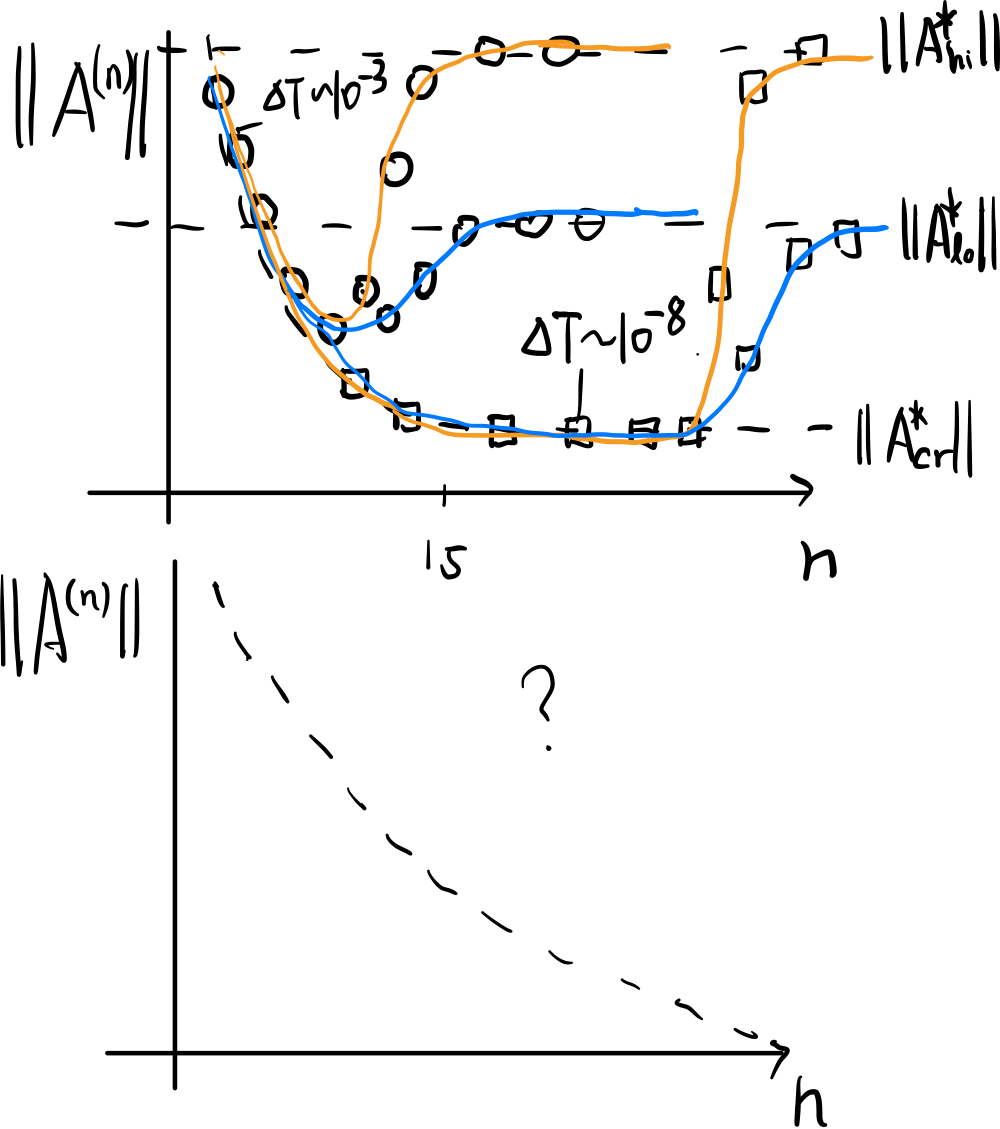
\includegraphics[width=7.5cm]{./figs/flowAnorm}
    \caption{\label{fig:flowAnorm}[\textbf{Add descriptions}]}
\end{figure}
%

The flow of the norms $\Vert A^{(n)} \Vert$ indicates Gilt-HOTRG is
capable of generating a correct RG flow of 2D Ising model in tensor
space shown schematically in Fig.~\ref{fig:tensorRGflow}(a). For exampe,
for bound dimension $\chi = 30$ and the hyper-parameter for Gilt process
$\epsilon_{\text{gilt}} = 6\times 10^{-6}$, Fig.~\ref{fig:flowAnorm}(a)
shows several RG flows of the tensor norms at different temperature. For
a fixed bound dimension $\chi$, there is an estimated critical
temperature $T_c^{[\chi]}$ at which the tensor
hits the critical surface and flows towards the critical fixed-point
tensor $(A^{[\chi]})^*_{\text{cr}}$. $T_c^{[\chi]}$ can be determined
using the bisection method, and for $\chi = 30$ the estimation error is
of order $\sim 10^{-6}$. At temperatures off by $\Delta T = \pm 10^{-3}$
from $T_c^{[30]}$, the tensor flows to the high temperature and the
low temperature trivial fixed-point tensors respectively before it comes
near to $(A^{[30]})^*_{\text{cr}}$. As $|\Delta T|$ becomes smaller to
order of $10^{-8}$, the tensor will stay in the vicinity of the critical
fixed-point tensor for a while and then flow away to the two trivial
fixed-point tensors. If $|\Delta T|$ becomes smaller further, the tensor
will stay longer near $(A^{[30]})^*_{\text{cr}}$. By comparsion, the
RG flow of $\Vert A^{(n)}\Vert$ generated by HOTRG with the same bound
dimension is displayed in Fig.~\ref{fig:flowAnorm}(b). The RG flow shows
that the RG equation in Eq.~\eqref{def:RGeqHOTRG} cannot exhibit a
critical fixed-point tensor or produce isolated trivial fixed-point
tensors. It is interesting to mention that the RG flow generated by TRG
has a similar behavior~\cite{Berker2008} to HOTRG for bound dimensions
$\chi > 10$.
%%
\begin{figure}[htb]
    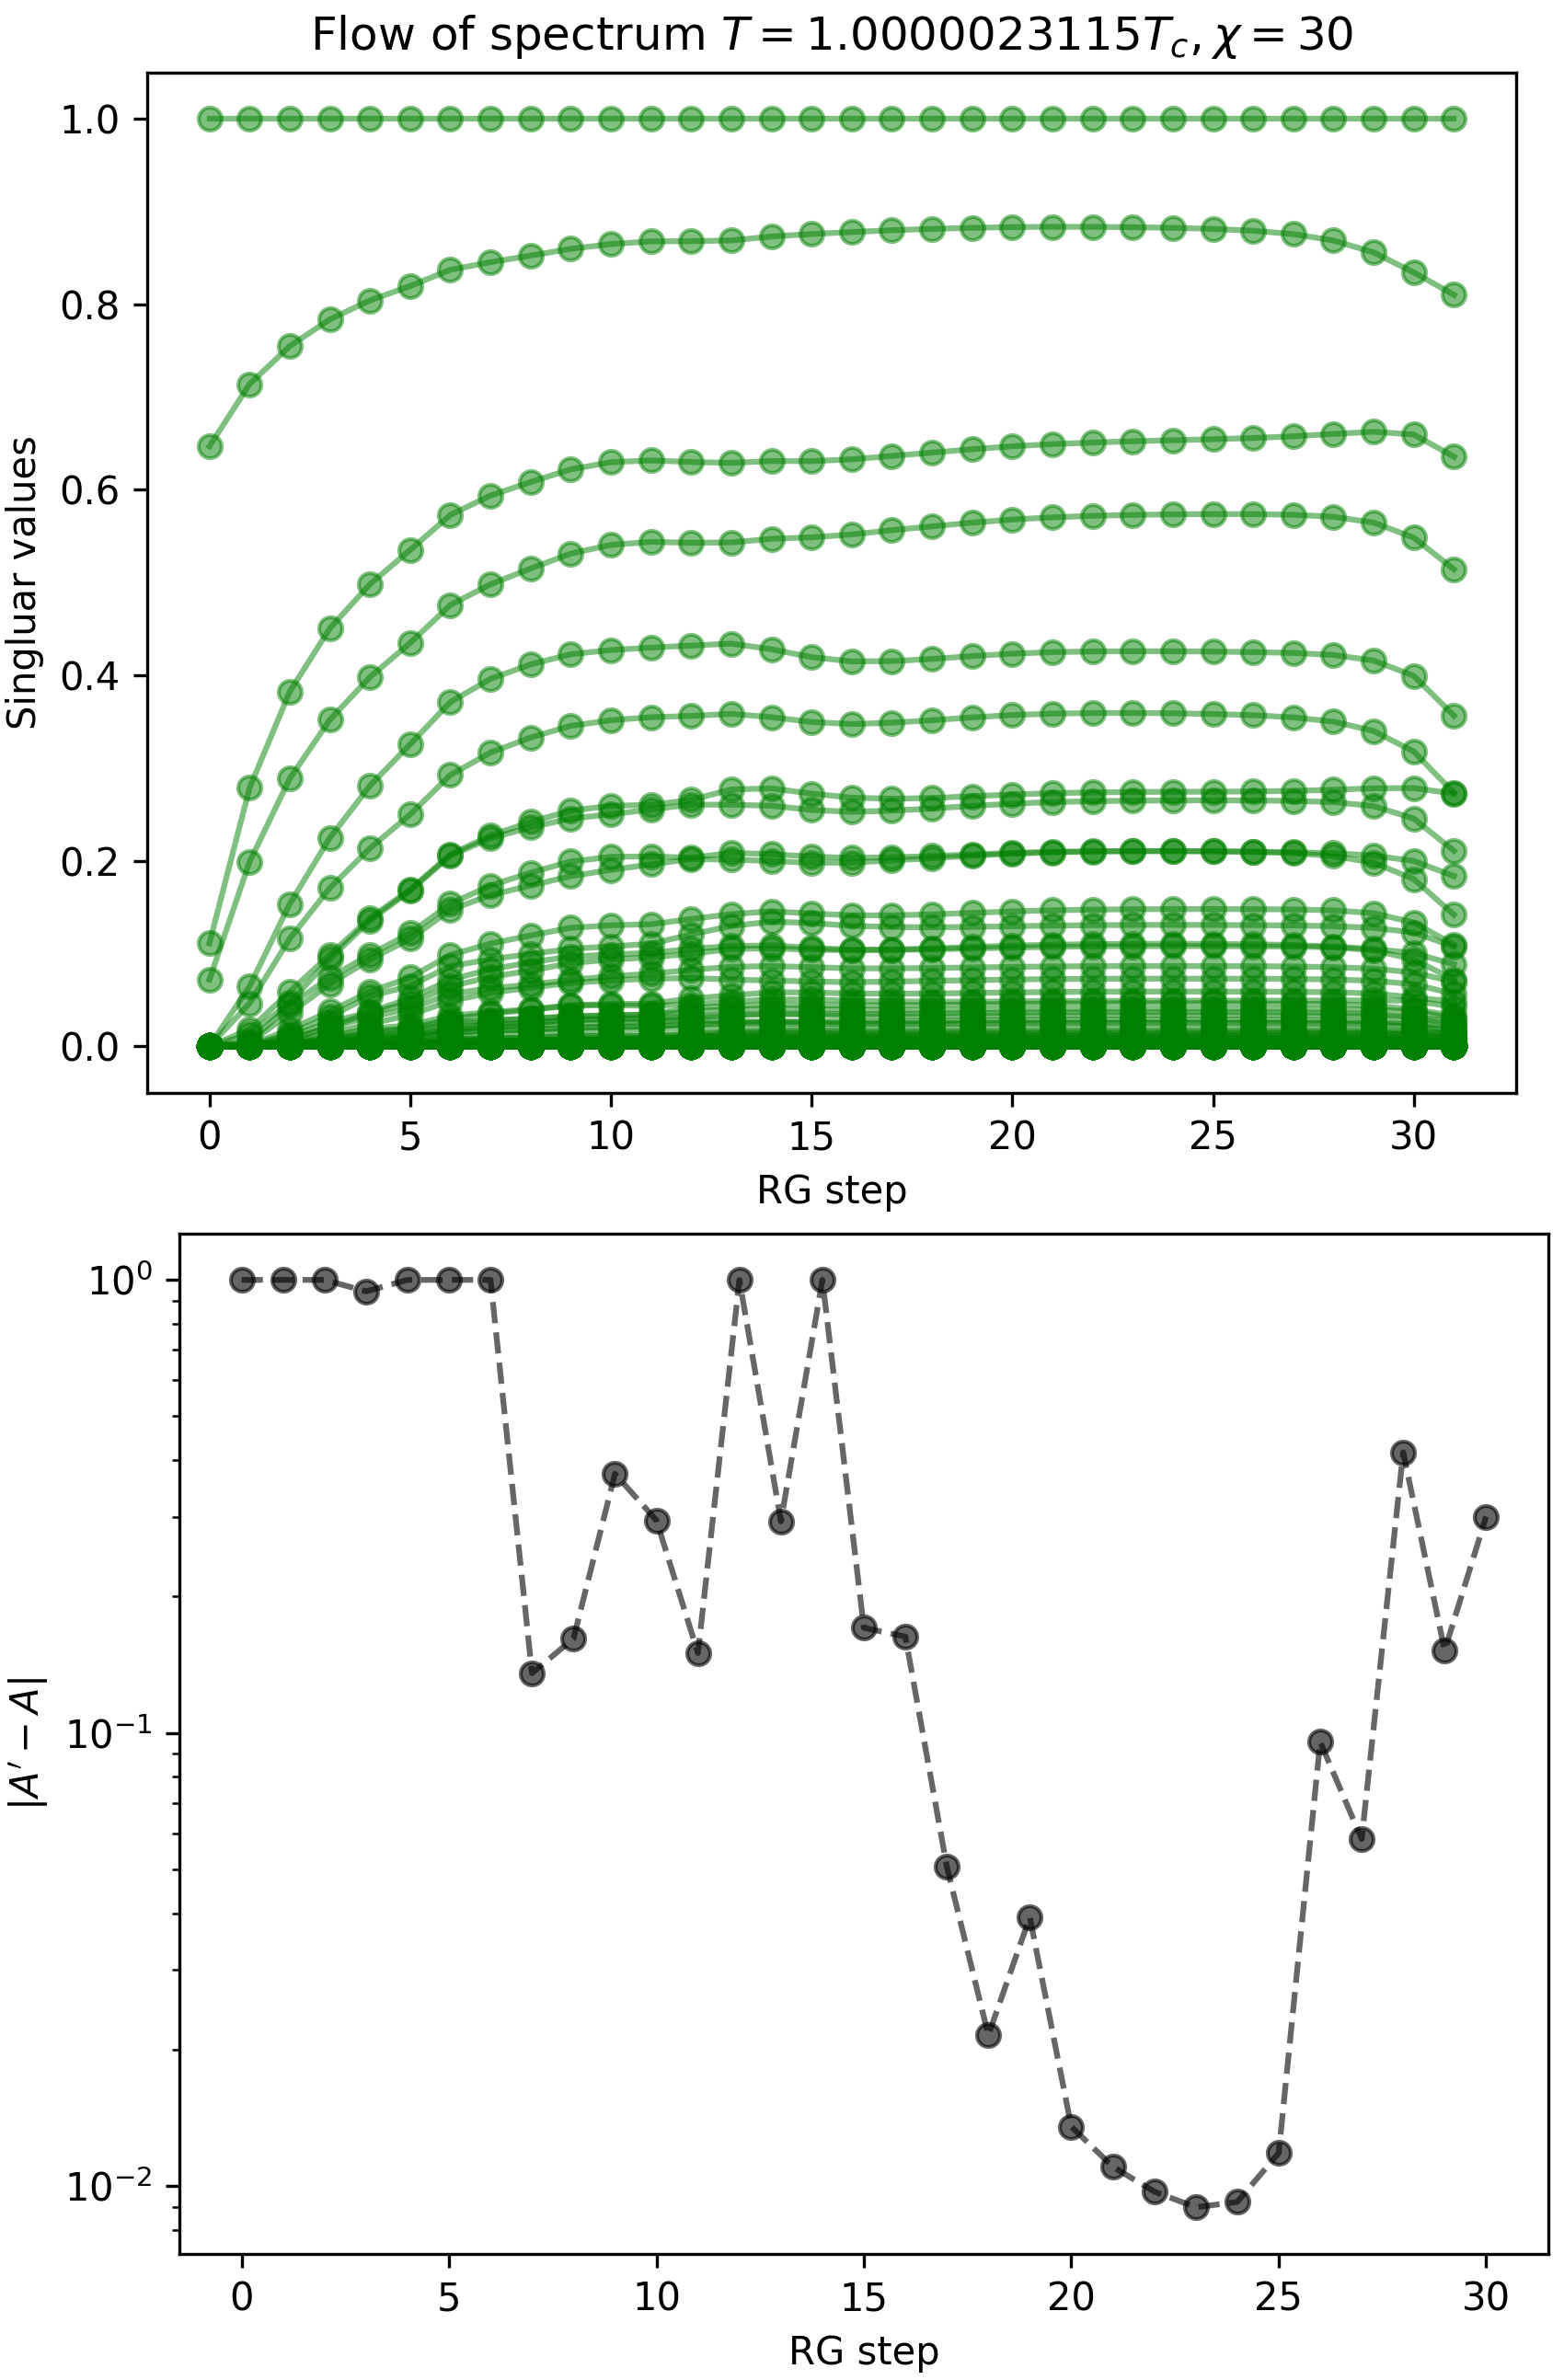
\includegraphics[width=7.5cm]{./figs/flowA}
    \caption{\label{fig:flowA}[\textbf{Add descriptions}]}
\end{figure}
%

To make sure that the plateau in the RG flow of $\Vert A^{(n)} \Vert$
gives a critical fixed-point tensor $(A^{[30]})^*_{\text{cr}}$ at the
estimated critical temperature $T_c^{[30]}$, we plot the singular values
of tensors $\mathcal{A}^{(n)}$ defined as
%
\begin{align}\label{def:Asvd}
    \begin{minipage}{2.0truecm}
        \centering
        \includegraphics[width=1.8truecm,clip]{./figs/Aold}
    \end{minipage}
    \svdeq
    \begin{minipage}{2.0truecm}
        \centering
        \includegraphics[width=1.8truecm,clip]{./figs/Asvd}
    \end{minipage}.
\end{align}
%
The flow of singular values in Fig.~\ref{fig:flowA}(a) indicates that we
indeed reach a non-trivial fixed-point tensor. The fixed-point tensor is
manifestly fixed numerically after adding the sign fixing step in
Gilt-HOTRG, which can be confirmed by checking the Frobenius norm of the
difference between the normalized tensors at successive RG steps $\Vert
\mathcal{A}^{(n+1)} - \mathcal{A}^{(n)}\Vert$, see
Fig.~\ref{fig:flowA}(b). The norm of the difference starts to decay
systematically at RG step $n = 14$, goes all the way down to the order
$\sim 10^{-2}$ at $n = 23$ and then increases when the tensor begins to
flow away from the critical fixed point.
%%
\begin{figure}[htb]
    \includegraphics[width=8.5cm]{./figs/scDim}
    \caption{\label{fig:scDim}[\textbf{Add descriptions}]}
\end{figure}
%
\begin{table}[h]%[H] add [H] placement to break table across pages
\caption{Scaling dimensions for relevant and marginal operators of 2D
Ising model at criticality from response analysis of the RG equation
of Gilt-HOTRG and from diagonalizing a
transfer matrix \`a la Gu and Wen~\cite{GuWen2009}, both with $\chi =
30, \epsilon_{\text{gilt}} = 6\times 10^{-6}$ at RG step $n =
22$.\label{table:scDim}} 
\begin{ruledtabular}
\begin{tabular}{ c c c c c c c c c }
Exact      & 0.125 & 1 & 1.125 & 1.125 & 2 & 2 & 2 & 2 \\
\hline
Resp. ana. & 0.127 & 1.009 & 1.125 & 1.128 & 2.002 & 2.004 & 2.068 &
2.073 \\
Tran. mat. & 0.125 & 1.009 & 1.130 & 1.148 & 1.313 & 1.457 & 1.558 & 
1.654
\end{tabular}
\end{ruledtabular}
\end{table}
%

We use the automatical differentiation implemented in
JAX~\cite{jax2018github} to linearize the RG equation of Gilt-HOTRG in
Eq.~\eqref{def:RGeqGiltHOTRG} and get the response matrix defined in
Eq.~\eqref{eq:respMatGiltHOTRG} at RG steps $n = 14,15,\ldots, 28$, when the
tensor is very close to the critical fixed-point tensor. The scaling
dimensions are extracted from the eigenvalues of the response matrix
according to Eq.~\eqref{eq:lambda2x}. In Fig.~\ref{fig:scDim}, we show
the first few scaling dimensions. The dashed lines are the exact
values~\cite{DiFrancesco1997}. For $\chi = 30$, the reponse analysis in
tensor space gives correct sclaing dimensions upto $2.125$. The results from
response analysis at $n = 14 \text{ and } 28$ is unreliable since $\Vert
\mathcal{A}^{(n+1)} - \mathcal{A}^{(n)}\Vert$ is of order $\sim 1$ (see
Fig.~\ref{fig:flowA}(b)). The results for $n = 15,16,\ldots,27$
indicates that the scaling dimensions from response analysis in tensor
space are reliable as long as the values of $\Vert \mathcal{A}^{(n+1)} -
\mathcal{A}^{(n)}\Vert$ have order of or smaller than $10^{-1}$. 
%

In Table~\ref{table:scDim}, we show the scaling dimensions for all
relevant and marginal operators from at the RG step $n = 22$, compared with
the results obtained by Gu and Wen's method~\cite{GuWen2009}. Both
methods have similar accuracy for scaling dimensions less or equal to
$1.125$, but Gu and Wen's method cannot produce higher scaling
dimensions. Our method can give two out of total four scaling dimension
$2$ accurately, but the remaining two are overestimated and more close
to $2.125$.
%

We end this section with a few remarks on the above calculation. First,
we impose the $\mathbb{Z}_2$ symmetry of the tensors~\cite{Singh2010SymTen,
Singh2011U1Ten} when generating the RG flow in tensor space. There are
three reasons. Only if the $\mathbb{Z}_2$ symmetry of the tensor is
imposed will the low-temperature fixed-point tensor be stable under RG.
Otherwise, it will flow to the high-temperature fixed point eventually
due to the numerical errors, which will make the bisection search of the
estimated critical temperature $T_c^{[\chi]}$ less convenient. The
second merit of symmetric tensors is that half of the gauge redundancy
can be automatically fixed (see Sec.~\ref{RespAnaGiltHOTRG}), making the
sign fixing procedure in Gilt-HOTRG easier. The third reason is to speed
up the computations. However, we roll back to ordinary tensors when
performing the response analysis, since the perturbations around the
fixed-point tensor do not have to preserve $\mathbb{Z}_2$ symmetry (for
example, the spin operator). The second remark is about the improvement
of the results of response analysis as the bound dimension
$\chi$ increases. 
% TODO

The final remark is that the Gilt-HOTRG
can be replaced with TNR~\cite{tnr,tnralgo} with few changes of other
procedures, since TNR is known to be capable of exhibiting critical
fixed-point tensors and its RG equation is similar to that of
Gilt-HOTRG. Considering the unprecedented accuracy of TNR, the
estimation of scaling dimensions might be much better. We develop the
response analysis in tensor space using Gilt-HOTRG in this paper in
order to prepare for the further applications on 3D systems.
%


\section{Summary and discussion}
\blindtext


% If you have acknowledgments, this puts in the proper section head.
\begin{acknowledgments}
Put your acknowledgments here.

\blindtext
\end{acknowledgments}

% Specify following sections are appendices. Use \appendix* if there
% only one appendix.
\appendix
\section{Optimization forms of eigenvalue problems\label{appd:opteig}}
\blindtext
\section{CDL tensors, HOTRG, and Gilt-HOTRG\label{appd:cdlHOTRG}}
\blindtext
\section{Gauge redundancy in Gilt-HOTRG\label{appd:gaugeFix}}
\blindtext


% Create the reference section using BibTeX:
\bibliography{tensorRGflow}

\end{document}
%
% ****** End of file apstemplate.tex ******

